%%%%%%%%%%%%%%%%%%%%%%%%%%%%%%%%%%%%%%%%%
% The Legrand Orange Book
% LaTeX Template
% Version 3.0 (January 26, 2022)
%
% This template originates from:
% https://www.LaTeXTemplates.com
%
% Authors:
% Vel (vel@latextemplates.com)
% Mathias Legrand (legrand.mathias@gmail.com)
%
% License:
% CC BY-NC-SA 4.0 (https://creativecommons.org/licenses/by-nc-sa/4.0/)
%
% Compiling this template:
% This template uses biber for its bibliography and makeindex for its index.
% When you first open the template, compile it from the command line with the 
% commands below to make sure your LaTeX distribution is configured correctly:
%
% 1) pdflatex main
% 2) makeindex main.idx -s indexstyle.ist
% 3) biber main
% 4) pdflatex main x 2
%
% After this, when you wish to update the bibliography/index use the appropriate
% command above and make sure to compile with pdflatex several times 
% afterwards to propagate your changes to the document.
%
%%%%%%%%%%%%%%%%%%%%%%%%%%%%%%%%%%%%%%%%%

%----------------------------------------------------------------------------------------
%	PACKAGES AND OTHER DOCUMENT CONFIGURATIONS
%----------------------------------------------------------------------------------------

\documentclass[
	12pt, % Default font size, select one of 10pt, 11pt or 12pt
	fleqn, % Left align equations
	a4paper, % Paper size, use either 'a4paper' for A4 size or 'letterpaper' for US letter size
	oneside, % Uncomment for oneside mode, this doesn't start new chapters and parts on odd pages (adding an empty page if required), this mode is more suitable if the book is to be read on a screen instead of printed
]{LegrandOrangeBook}

% Book information for PDF metadata, remove/comment this block if not required 
\hypersetup{
	pdftitle={Title}, % Title field
	pdfauthor={Author}, % Author field
	pdfsubject={Subject}, % Subject field
	pdfkeywords={Keyword1, Keyword2, ...}, % Keywords
	pdfcreator={LaTeX}, % Content creator field
}


\newsavebox{\fminipagebox}
\NewDocumentEnvironment{fminipage}{m O{\fboxsep}}
 {\\\kern#2\noindent\begin{lrbox}{\fminipagebox}
  \begin{minipage}{#1}\ignorespaces}
 {\end{minipage}\end{lrbox}%
  \makebox[#1]{%
    \kern\dimexpr-\fboxsep-\fboxrule\relax
    \fbox{\usebox{\fminipagebox}}%
    \kern\dimexpr-\fboxsep-\fboxrule\relax
  }\\\kern#2
 }

\addbibresource{sample.bib} % Bibliography file

\definecolor{ocre}{rgb}{0.5, 0.5, 0.5} % Define the color used for highlighting throughout the book
\providecommand{\tightlist}{%
  \setlength{\itemsep}{0pt}\setlength{\parskip}{0pt}}
\chapterimage{orange1.jpg} % Chapter heading image
\chapterspaceabove{6.5cm} % Default whitespace from the top of the page to the chapter title on chapter pages
\chapterspacebelow{6.75cm} % Default amount of vertical whitespace from the top margin to the start of the text on chapter pages

%----------------------------------------------------------------------------------------

\begin{document}

%----------------------------------------------------------------------------------------
%	TITLE PAGE
%----------------------------------------------------------------------------------------

\titlepage % Output the title page
	{\includegraphics[width=\paperwidth]{background.pdf}} % Code to output the background image, which should be the same dimensions as the paper to fill the page entirely; leave empty for no background image
	{ % Title(s) and author(s)
		\centering\sffamily % Font styling
		{\Huge\bfseries Money \& Trust in Metaverses\par} % Book title
		\vspace{16pt} % Vertical whitespace
		{\LARGE Bitcoin and stablecoins in  social XR\\}  % Subtitle
		\vspace{24pt} % Vertical whitespace
		{\large \textbf{Draft product design for Flossverse and PathwayXR}\par} % Author name
	}

%----------------------------------------------------------------------------------------
%	COPYRIGHT PAGE
%----------------------------------------------------------------------------------------

\thispagestyle{empty} % Suppress headers and footers on this page

~\vfill % Push the text down to the bottom of the page

\noindent \href{https://creativecommons.org/licenses/by-nc/4.0/}{Attribution-NonCommercial 4.0 International (CC BY-NC 4.0) }\\ 2022 John O'Hare \& Allen Fairchild \& Umran Ali\\ % Copyright notice

\noindent \textsc{Published by john@xrsystems.uk (R\&D Lead - Pathway)}\\ % Publisher

\noindent \textsc{\href{https://github.com/flossverse/origin/blob/draft/Book/metaverseBTC.pdf}{Raw GitHub hyperlink}}\\ % URL

\noindent 
You are free to:
\begin{itemize}
\item Share — copy and redistribute the material in any medium or format
\item Adapt — remix, transform, and build upon the material
\end{itemize}
The licensor cannot revoke these freedoms as long as you follow the license terms.\\
Under the following terms:
\begin{itemize}
\item Attribution — You must give appropriate credit, provide a link to the license, and indicate if changes were made. You may do so in any reasonable manner, but not in any way that suggests the licensor endorses you or your use.
\item NonCommercial — You may not use the material for commercial purposes.
\item No additional restrictions — You may not apply legal terms or technological measures that legally restrict others from doing anything the license permits.
\end{itemize}
\noindent \textit{First printing, March 2022} % Printing/edition date

%----------------------------------------------------------------------------------------
%	TABLE OF CONTENTS
%----------------------------------------------------------------------------------------

\pagestyle{empty} % Disable headers and footers for the following pages

\tableofcontents % Output the table of contents

\listoffigures % Output the list of figures, comment or remove this command if not required

\listoftables % Output the list of tables, comment or remove this command if not required

\pagestyle{fancy} % Enable default headers and footers again

\cleardoublepage % Start the following content on a new page

%----------------------------------------------------------------------------------------
%	PART
%----------------------------------------------------------------------------------------

\part{State of the art and proposal}

%----------------------------------------------------------------------------------------
%	SECTIONING EXAMPLES CHAPTER
%----------------------------------------------------------------------------------------

\chapterimage{orange2.jpg} % Chapter heading image
\chapterspaceabove{6.75cm} % Whitespace from the top of the page to the chapter title on chapter pages
\chapterspacebelow{7.25cm} % Amount of vertical whitespace from the top margin to the start of the text on chapter pages

%------------------------------------------------

\section{Conflict of interest statements}
\input{conflicts}
\chapter{Introduction}
\section{Overview}
As human beings, we have always relied on certain social constructs to guide our interactions and transactions with one another. Money and trust are two such constructs that have played a vital role in shaping our societies, and the way we live our lives. However, the digital age has brought with it new challenges that are testing the foundations of these social norms.\par
In a world where we are increasingly connected through the internet and able to communicate with people from all corners of the globe, the concept of money and trust is changing. Gone are the days of the village structure in which we evolved, where personal relationships and face-to-face interactions were ubiquitous. Now, we are faced with the prospect of working and interacting one another, and also with artificial intelligence actors that seem subjectively real, all while navigating the complexities of a global mixed reality.\par
This transition to a more efficient and interconnected world has the potential to bring about great benefits, but it also presents us with an enormous challenge. The chaotic and intangible mix of value, trust, socialisation, generative art, and AI chat actors, is not yet well understood, and it will take time for us to adapt to this new way of living and interacting with one another.\par
We initially wanted to explore exciting new developments in the transmission of value, and trust, in `digital society'. The problem is that each of these topics alone are enormously complex, and the intersections seem to be more so. We have been researching the current state-of-the-art, and the emerging consensus narrative, to try to figure out how the collision of these technologies might serve our virtual production workflows (Figure \ref{fig:vprobot}). As we worked on this research the Cambrian explosion of generative AI added an incredibly important new strand to our investigation.\par
Over the course of a couple of years the focus of the work has developed, and refined. Our tool-kit, as it stands, supports inclusive human creativity and economic exchange, especially for emerging markets and especially perhaps \href{https://www.afrobitcoin.org/}{Africa}. There is a huge proportion of human creativity currently excluded from media production pipelines due to gatekeepers of knowledge, access to identity proofs, and financial infrastructure that is taken for granted in the richer nations. This inclusion will be accomplished for the most part through integration of open source machine learning and AI tools, but this field quite new, and that part of the work is under developed.\par

%\textbf{\hyperref[sec:tldr]{If at this stage you want to skip straight to the TL;DR for the whole book then click this bold text}.}\par
\begin{figure}
  \centering
   \includegraphics[width=\linewidth]{vprobot}
 \caption{In camera VFX virtual production}
    \label{fig:vprobot}
\end{figure}


\section{Introduction}
This document presents a high level view of technologies and their potential within the emergent Web3 and metaverse narrative, focusing around the transmission of value within and across such global networks, with a further focus on the Bitcoin monetary network. It was written to organise the thoughts of the authors, who were unfamiliar with Bitcoin technologies until recently.\par
As adoption of these technologies increases it will be necessary for people, and AI actors, to pass economic value between themselves. These `goods and services' interactions, within the virtual social spaces should be underpinned by a trust system, which scales globally and presents low friction. Current secure international payment rails are poorly suited to such interactions; indeed it is likely with legacy systems, that parties would be forced to leave the metaverse application, and instead navigate their banking applications to exchange value with overseas entities in a secure fashion. This might conceivably take several days.\par 
Fortunately, the whole landscape of money and \href{https://www.omfif.org/futureofpayments2021/}{value transfer is changing}. Huge global financial players are entering the space. HSBC have \href{https://sandboxgame.medium.com/hsbc-to-become-the-first-global-financial-services-provider-to-enter-the-sandbox-c066e4f48163}{just bought} metaverse `land' in The Sandbox, JP Morgan have \href{https://www.forbes.com/sites/ronshevlin/2022/02/16/jpmorgan-opens-a-bank-branch-in-the-metaverse-but-its-not-for-what-you-think-its-for/?sh=2fbd1e90158d}{opened a `lounge'} in another. The worlds largest hedge fund Bridgewater is stepping into \href{https://uk.finance.yahoo.com/news/bitcoin-latest-price-crypto-ray-dalio-bridgewater-investment-fund-ethereum-094946686.html}{acquisition of digital assets}, and the world's largest pension fund manager Blackrock \href{https://blog.coinbase.com/coinbase-selected-by-blackrock-provide-aladdin-clients-access-to-crypto-trading-and-custody-via-b9e7144f313d}{partnered with Coinbase} and is adding these asset to their management engine (which manages tens of trillions of dollars). Fidelity asset management are about to add \href{https://www.wsj.com/articles/fidelity-to-allow-retirement-savers-to-put-bitcoin-in-401-k-accounts-11650945661}{Bitcoin to their pension plans} and are offering a \href{}{dedicated metaverse tradable fund}, while \href{https://www.citivelocity.com/citigps/metaverse-and-money/}{Citigroup have a minisite} dedicated to ``Metaverse and Money''. The front page of Goldman Sachs recently says it all (Figure \ref{fig:goldmanFront}).\par
\begin{figure}[ht]\centering % Using \begin{figure*} makes the figure take up the entire width of the page
	\includegraphics[width=0.5\linewidth]{goldmanFront}
	\caption{The landing page of global\\financial giant Goldman Sachs shows the hype.}
	\label{fig:goldmanFront}
\end{figure}
In Gartners \href{https://www.itp.net/emergent-tech/gartner-says-nfts-metaverse-web3-will-expand-immersive-experiences}{2022 hype cycle report} one of their three ``trend themes'' says: \textit{``The future of digital experience is immersive. A collection of emerging technologies supports such experiences through dynamic virtual representations, environments and ecosystems of customers and people, as well as new modes of user engagement. With these technologies, individuals can control their own identities and data and experience virtual ecosystems that can be integrated with digital currencies. These technologies help reach customers in new ways to strengthen or open new revenue streams.
The technologies to watch that deliver evolving and expanding immersive experiences are metaverse, non-fungible tokens (NFTs), super apps and Web3, decentralized identity, digital humans, digital twin of the customer and internal talent marketplaces.''}\par
Of their recent investments KPMG global said: \textit{``We've invested in a strong cryptoassets practice and we will continue to enhance and build on our capabilities across Decentralized Finance (DeFi), Non-Fungible Tokens (NFTs) and the Metaverse, to name a few''}. This is not to say that all fund managers are so positive. PGIM who manage over a trillion pounds globally have come out very strongly against the technology, with a \href{https://www.pgim.com/megatrends/cryptocurrency-investing/bitcoin?}{slew of reports} to warn off investors (Figure \ref{fig:pgim}).\par
\begin{figure}[ht]\centering 	\includegraphics[width=0.5\linewidth]{pgim}
	\caption{PGIM cite the `digiconomist' paper}
	\label{fig:pgim}
\end{figure}
It's possible that for such organisations it makes better business sense to take a punt on hype bubbles like this, than to do a proper due diligence with a team of internal staff who understand their business. These endorsements should be taken with a large pinch of salt. As \href{https://newsletter.fintechtakes.com/p/metaverse-branches?s=r}{Alex Johnson says}: \textit{``At some point in the future, it’s possible that the digital worlds being built today will have aggregated sufficient user attention and engagement that financial services companies will need to invest in the metaverse as an acquisition and customer service channel. But we’re not there yet. Until the metaverse is a little less empty, resist the temptation to colonize it with branches and billboards.''}\par
Meanwhile, Meta (ex Facebook) are launching their own \href{https://archive.ph/coyp2}{META Web3 and metaverse} token (after abandoning Libre, their global cryptocurrency), and \href{https://www.cnbc.com/2022/05/06/googles-cloud-group-forms-web3-product-and-engineering-team.html}{Google} have \href{https://blog.youtube/inside-youtube/innovations-for-2022-at-youtube/}{recently blogged}: \textit{``Web3 also opens up new opportunities for creators. We believe new technologies like blockchain and NFTs can allow creators to build deeper relationships with their fans. Together, they'll be able to collaborate on new projects and make money in ways not previously possible. For example, giving a verifiable way for fans to own unique videos, photos, art, and even experiences from their favourite creators could be a compelling prospect for creators and their audiences. There's a lot to consider in making sure we approach these new technologies responsibly, but we think there's incredible potential as well. Finally, we couldn't have a piece about innovation without touching on the metaverse! We're thinking big about how to make viewing more immersive. ''}\par
It's already the case that the recent bubble of \href{https://www.forbes.com/sites/paultassi/2022/03/10/interest-in-nfts-and-the-metaverse-is-falling-fast/?}{hype is dwindling}, but the enormous investment into teams and startups will potentially bear fruit in the next couple of years, and this perhaps has implications for small and medium-sized enterprises (SMEs). \par
In the UK the government has stated it's ambition to be a \href{https://www.gov.uk/government/news/government-sets-out-plan-to-make-uk-a-global-cryptoasset-technology-hub}{global cryptoasset technology hub}, and announced plans for the Royal Mint to issue a (novelty) NFT. Like the assertion by major global businesses it is too early to tell how `sticky' these claims are, but the UK legal system is clear in it's view that all crypto assets \href{https://blockchain.bakermckenzie.com/2020/02/03/uk-court-confirms-bitcoins-status-as-property/}{are `property'}.\par
A Law Commission consultation on ``digital assets'' \href{https://s3-eu-west-2.amazonaws.com/lawcom-prod-storage-11jsxou24uy7q/uploads/2022/07/Digital-Assets-Summary-Paper-Law-Commission-1.pdf}{has proposed a new \textbf{third category} of property}:
\textit{\begin{itemize}
\item it is composed of data represented in an electronic medium, including in the
form of computer code, electronic, digital or analogue signals;
\item it exists independently of persons and exists independently of the legal system;
\item it is rivalrous such that use by one  prejudices the ability of others;
\end{itemize}
}
Consensus seems to be that this is a thorough paper, and demonstrates strong knowledge of digital assets by the authors. \par
Gartner's \href{https://en.wikipedia.org/wiki/Gartner_hype_cycle}{hype cycle} 2022 features \href{https://www.gartner.com/en/articles/what-s-new-in-the-2022-gartner-hype-cycle-for-emerging-technologies}{Web3, distributed identity, NFTs, and Metaverse} and can be seen in Figure \ref{fig:gartners}.
\begin{figure}[ht]\centering % Using 
	\includegraphics[width=0.9\linewidth]{gartners}
	\caption{The Gartners Hype Cycle for 2022.}
	\label{fig:gartners}
\end{figure}
With all this attention it seems timely to explore the potential of recent technologies, which can address metaverse interactions in \textit{business to business} (B2B), \textit{business to customer} (B2C), and the newer C2C (social commerce; \textit{creator to consumer, customer to customer, consumer to consumer\cite{jones2008trust})}. Figure \ref{fig:landscapevenn} demonstrates how some of these domains intersect.\par
This book seeks to overview and explain the available open source technologies. It supports an open source \href{https://github.com/flossverse/origin}{github repository} which enables SMEs to access these emergent platforms and ecosystems. It aims to build toward a minimum viable product for trust minimised transfer of value within a social immersive space.\par
Referencing is in two styles; academic works and books are numeric, while opinion pieces, gray statistics, and pertinent news articles are hyperlinked from the text. This hybrid style yields about twice the citation density of a normal PhD thesis, which is a lot. For this reason the normal blue hyperlink colour was eschewed in favour of a more aesthetic ``gray''. There is also a version of the PDF which complies with accessibility best practice if this is a problem.  \par 
\subsection{Notes on progress}
\textbf{This version of the book is being overhauled to improve the focus, and expand the virtual production use cases. It may be inconsistent and look scrappy until this message is removed.}\
\chapter{Decentralisation \& Web3}
\input{02_decentralised_web}

\chapter{DLT, Blockchain, and Bitcoin}
Distributed ledger technology (DLT) is a data structure distributed across multiple managing stakeholders. A subset of DLT is blockchain, which is a less efficient, immutable data structure with a slightly different trust model. Rauchs et al. of the Cambridge Centre for Alternative Finance provide a detailed taxonomy and conceptual framework \cite{rauchs2018distributed}. It can be seen in their paper that the definitions are somewhat unclear in literature.\par
DLT, and especially blockchain, are rapidly gaining ground in the public imagination, within financial technology companies (FinTech), and in the broader corporate world. \par
The technology and the global legislative response are somewhat immature, and misapplications of both technologies are commonplace. \par
Distributed trust models emerged from cryptography research in the 1970s when Merkle, Diffie, and Hellman at Stanford worked out how to \href{https://medium.com/swlh/understanding-ec-diffie-hellman-9c07be338d4a}{send messages online} without a trusted third party \cite{diffie1976new,merkle1978secure}.\par
Soon after the 1980s saw the emergence of the cypherpunk activist movement, as a reaction to the emerging surveillance state \cite{burnham1983rise, chaum1985security}, a topic which is expanded for this moment in a later chapter. These early computer scientists in the USA saw the intersectionality between information, computation, economics, and personal freedom \cite{lavoie1990prefatory}. Online discussion in the early nineties foresaw the emergence of trans-national digital markets, what would become the WWW \cite{salinCosts, cypherPunkMailList}. The issues of privacy %(https://nakamotoinstitute.org/static/docs/cypherpunk-manifesto.txt) 
 and the exchange of digital value (digital / ecash) %(https://www.wired.com/1994/12/emoney/  https://www.cs.ru.nl/~jhh/pub/secsem/chaum1985bigbrother.pdf) 
 were of foremost importance within these discussions %(https://www.wired.com/1994/12/emoney/), 
 and while privacy was within reach thanks to \href{https://www.openpgp.org/about/history/}{``public/private key pairs''}, 
 ecash proved to be a more difficult problem. \par
Adam Back's 1997 `hashcash' \cite{back2002hashcash} paved the way for later work by implementing the concept of what would become `proof of work' \cite{dwork1992pricing, jakobsson1999proofs}. This was built upon by Dai \cite{dai1998b}, Szabo \cite{szabo1997formalizing}, Finney \cite{callas1998openpgp}, and Nakamoto amongst others. In all it took 16 years of collaboration on the mailing lists (and dozens of failed attempts) to attack the problem of trust-minimised, distributed, digital cash. The culmination of these attempts was Bitcoin \cite{Nakamoto2008}. This is illustrated by Dan Held in Figure \ref{fig:prehistory}. This is now a wider ecosystem of technologies and societal challenges (Figure \ref{fig:bitcointopics}). 

\begin{figure}
  \centering
    \includegraphics[width=\linewidth]{prehistory}
  \caption{Dan Held: \href{https://www.danheld.com/blog/2019/1/6/planting-bitcoinsoil-34}{Bitcoin prehistory} used with permission.}
  \label{fig:prehistory}
\end{figure}

\begin{figure}
  \centering
    \includegraphics[width=\linewidth]{bitcointopics}
  \caption{\href{https://twitter.com/djvalerieblove/status/1514703620272394243/photo/1}{Bitcoin Topics} used with permission @djvalerieblove.}
  \label{fig:bitcointopics}
\end{figure}

There is enormous complexity and scope, as seen in Figure \ref{fig:venn}, and yet genuinely useful products are elusive.
\begin{figure*}[ht]\centering % Using \begin{figure*} makes the figure take up the entire width of the page
	\includegraphics[width=\linewidth]{venn}
	\caption{\href{https://unchained.com/blog/blockchain-spectrum/}{Intersecting disciplines}. Reused with permission \href{https://unchained.com/}{Dhruv Bansal}}
	\label{fig:venn}
\end{figure*}
It is surprisingly hard to pin down a simple explanation for the features which define a blockchain. These ``key takeaway'' \href{https://www.investopedia.com/terms/b/blockchain.asp}{from Investopedia} are a neat summary however.\par
\textit{\begin{itemize} \item Blockchain is a specific type of database. \item It differs from a typical database in the way it stores information; blockchains store data in blocks that are then chained together. \item As new data comes in it is entered into a fresh block. Once the block is \href{https://bits.monospace.live/}{filled with data} it is chained onto the previous block, which makes the data chained together in chronological order. \item Different types of information can be stored on a blockchain but the most common use so far has been as a ledger for transactions. \item In Bitcoin’s case, blockchain is used in a decentralized way so that no single person or group has control—rather, all users collectively retain control. \item Decentralized blockchains are ``append only''. In effect this means that the data entered becomes irreversible over time. For Bitcoin, this means that simple economic transactions are permanently recorded and viewable to anyone. \end{itemize}}
In principle blockchains provide a \textbf{differentiated trust model}. With a properly distributed system a blockchain can be considered ``trust-minimised'', though certainly not risk minimised. This is important for some, but not all people. There is not much emboldening of text within this book. If you start to question the whole reason for this `global technology revolution' then it always comes back to those three words. \par
It can in fact be argued that the whole concept of distributed cryptographic blockchains is \href{https://www.trailofbits.com/reports/Unintended_Centralities_in_Distributed_Ledgers.pdf}{somewhat strained}, as the vast majority of the technology offerings are not distributed, and worse, meaningful distribution may indeed be practically impossible without a trusted third party \cite{kwon2019impossibility}. ``There are many scenarios where \href{https://calpaterson.com/blockchain.html}{traditional databases} should be used instead''\cite{casino2019systematic}.\par
\section{What's this for sorry?}
The proponents of blockchains argue, that in an era when data breaches and corporate financial insolvency intersect with a collapse in trust of institutions, it is perhaps useful to have an alternative model for storage of data, and value. That seems like a lot of effort for a questionable gain. It's far more likely it's simply speculation.\par 
While writing this book the questions of `what is this \textit{really for} and how can it possibly be worth it', came up again and again. In truth it's a very difficult question, without a clear enough answer. It's beyond the scope of this book to figure this out properly, but references to advantages and disadvantages will be made throughout.\par  
It seems that the engineers who created Bitcoin wanted very much to solve a technical problem they saw with money (from their understanding of it), and the transmission of money digitally. As the scale and scope have increased so has the \href{https://medium.com/@nic__carter/visions-of-bitcoin-4b7b7cbcd24c}{narrative evolved} as seen in Figure \ref{fig:Evolving}, but it's never really kept pace with the level of the questions posed. \par
\begin{figure*}[ht]\centering % Using 
	\includegraphics[width=\linewidth]{evolvingnarrative}
	\caption{The narrative use of Bitcoin has evolved, by Nic Carter and Hasufly.}
	\label{fig:Evolving}
\end{figure*}
A cost benefit analysis that excludes speculative gains seems to fail for pretty much all of blockchain/DLT. Bitcoin is more subtle as it possibly \textit{can} circumvent the legacy financial systems. This still leaves huge questions. To quote others in the space, is Bitcoin now the iceberg or the life raft? \par 
For the most developed defence of the technology as it stands in from a Western perspective, in this moment, Gladstein (\href{https://www.financialinclusion.tech/}{and others}) offer a vision for the asset class, in the 87\% of the world he says don't have access to the technology infrastructure benefits enjoyed by the developed west \cite{gladsteincheck2022} (Figure \ref{fig:walledworld}). 
\begin{figure*}[ht]\centering % Using \begin{figure*} makes the figure take up the entire width of the page
	\includegraphics[width=\linewidth]{walledworld}
	\caption{We live in an increasingly \href{https://www.tni.org/en/walledworld}{walled world} (tni, rights requested)}
	\label{fig:walledworld}
\end{figure*}
He points to Block and Wakefield Research's report which finds those living under financially oppressive regimes are the most optimistic about the technology as in Figure \ref{fig:optimism}. This argument is suggestive of huge and untapped markets for services which may be accessible to developed nations through telepresence/metaverse interfaces, and which may increase equity of access to opportunity elsewhere. To put some figures against this:
\begin{itemize}
\item Nigeria has the highest number of crypto owners in the world in 2022 with 45\% of its population owning or using cryptocurrency.
\item Thailand occupies the second space with 44\% of its population reported to be using or owning cryptocurrency.
\item Turkey has 40\% of its population owning and using cryptocurrency in 2022, equal to over 33 million people.
\item Argentina occupies the fourth position with an ownership and usage rate of 35\% in 2022, representing almost 16 million people.
\item United Arab Emirates has 34\% of the population owning or using cryptocurrency in 2022, representing almost 10 million people.
\item Philippines is ranked sixth with a 29\% adoption rate.
\end{itemize}
\begin{figure*}[ht]\centering % Using \begin{figure*} makes the figure take up the entire width of the page
	\includegraphics[width=\linewidth]{optimism}
	\caption{\href{https://twitter.com/gladstein/status/1532054253673406464}{``This new chart from Block is financial privilege visualized.''}}
	\label{fig:optimism}
\end{figure*}
Gladstein's is a carefully developed and well researched book, but is \href{https://bitcoinmagazine.com/culture/imf-world-bank-repress-poor-countries}{written from the western perspective} of (just) Bitcoin `being the raft'. Later in this book we will consider if it might be the iceberg, but this is not the domain expertise we offer in this book. It is crucial to note that Gladstein has vociferous detractors within Africa. It seems entirely possible he's another grifter as suggested by Kimani: \textit{``Gladstein is a charlatan who makes his living by selling the image of a global south that is corrupt, entirely lacking in rational thinking and needing a saviour, like him to swoop in and save us from our floundering selves. He exploits on tired and unproven stereotypes, cherry picks data while ignoring mountains of evidence that disprove him. Because he knows that as the perceived ``morally superior'' ``right thinking'' western superior coming to save, he will mostly go unchallenged. It's a grift, an old grift that many like him have turned into an industry. Where they earn tax free income by selling a delusion and fetish to their western audience who need to think the global south is a failure of the human experience. He is trying to set himself up as some gate keeper and king maker in the Global South. He knows that the next phase of growth is. So he wants to make sure that westerners looking to invest in the global south  see him as some ``expert'' and ask for his unfounded opinions. People like him run global morality extortion rings. How so? Simple: By purporting to know and be the keeper of global south morality, he will use his words to bless or curse your business, well, unless you make a generous donation to his foundation. These are scare tactics employed by charlatans to run tax-evading PR entities, thinly veiled as ``human rights'' organisations. If you are not on his side, he will slander you and your organisation. If you ensure you promote him and his ambitions, he anoints you as the good guy! He is trying to play the role that the Vatican and other corrupt religious organisations played in the 1800. Turning morality into a commodity that can be purchased from his market place: We decide who is good and who is bad and who can do business and who can't. For a ``donation''. He is not the first and he will not be the last. It's a growing industry, driven by shrewd westerners who know that they can sell racial stereotypes back home, but as long as they claim they are the one's helping or saving the coloured peoples from themselves.''} \par
%To further contextualise this \href{https://www.youtube.com/watch?v=BRQIMjZLMDk}{Mike Novogratz} claims the adoption figures at the top of the page. 
\href{https://dailyhodl.com/2022/05/04/crypto-winter-unlikely-as-astonishing-user-growth-dwarfs-internet-adoption-rate-macro-guru-raoul-pal/}{Raoul Pal of RealVision} says: \textit{Crypto adoption is now massively outperforming the internet. It’s been growing at about 165\% a year versus 85\% for the internet for the same period of time now.} According to analytics company Chainalysis; growth is fastest in the Middle east and North Africa (Figure \ref{fig:grow}). \par
\begin{figure*}[ht]\centering % Using 
	\includegraphics[width=\linewidth]{grow}
	\caption{Rapid growth is mainly outside of `Western Markets'}
	\label{fig:grow}
\end{figure*}
Thanks to a natural fit with strong encryption, and innate resistance to censorship by external parties, these systems do lend themselves well to `borderless' applications, and are somewhat resistant to global regulation (for good or ill). Given the rates of adoption seen in Figures \ref{fig:grow}, \ref{fig:ownership}, \ref{fig:userFigures}, and \ref{fig:euroInvest} it seems that this stuff is coming regardless of their usefulness to the developed world. If we are to take this as a given then we can perhaps logically infer that finding a use case for the technology is important, somewhat irrespective of other arguments. This provides us an opportunity to explore for metaverse applications, and this will be the focus.
\begin{figure*}[ht]\centering % Using 
	\includegraphics[width=\linewidth]{ownership}
	\caption{Rapid growth is mainly outside of `Western Markets' - 2}
	\label{fig:ownership}
\end{figure*}
\begin{figure*}[ht]\centering % Using 
	\includegraphics[width=\linewidth]{userFigures}
	\caption{Regular user numbers are surprisingly high.}
	\label{fig:userFigures}
\end{figure*}

\begin{figure*}[ht]\centering % Using 
	\includegraphics[width=\linewidth]{euroinvest}
	\caption{European crypto investment vs funds stocks and bonds from \href{https://github.com/gilbertfontana/DataVisualization}{Fontana} at \href{https://www.visualcapitalist.com/cp/crypto-popularity-in-europeans-union-nations/}{VisualCaptialist}}
	\label{fig:euroInvest}
\end{figure*}

%\begin{table}[]
\begin{tabular}{|l|r|l|r|}
\end{tabular}
\end{table}

\section{A panoply of tech}
Within DLT/blockchain there seem to be as many opinions on the value of the technology as there are implementations. A host of well engineered open source code repositories makes the cost of adoption relatively low. \par%Unfortunately there are many more repositories that look very similar and essentially scams.\par
There are thousands of different `chains' and many more tokens which represent value on them. A majority of these are code forks of earlier projects. Most \href{https://99bitcoins.com/deadcoins/}{are defunct} yet still have some residual `value' locked up in them as a function of their `distributed' tokens. \par 
Because the space is comparatively new, subject to \href{https://www.esma.europa.eu/press-news/consultations/call-evidence-dlt-pilot-regime}{scant regulation}, and often open source, it is possible to clone a github, change a few lines of code, and front it with a website in order to create `scams', and this happens frequently \cite{golumbia2020cryptocurrency}.\par
%An earlier version of this book talked about the opportunities and challenged with the dominant ``smart chain'' network; Ethereum. These pages can be \href{https://raw.githubusercontent.com/flossverse/product/draft/Book/03_ether.tex}{found in the github}, but were removed to improve the focus of this design. Now that Ethereum has transitioned to a more energy efficient consensus model our choice to dismiss the technology has become even more clear, and this will be explained later in the section.
The following sections give an overview of the major strands of the technology. First is Ethereum, mainly to discount it's use for our needs, and move on to more appealing options.

\section{Ethereum}
Ethereum \cite{buterin2013ethereum} is the second most \href{https://www.crypto51.app/}{secure} public blockchain (\href{https://howmanyconfs.com/}{by about 50\%})\cite{sayeed2019assessing}, and second most valuable by \href{https://coinmarketcap.com/}{market capitalisation} (though this comparison is somewhat stretched). It is the natural connection from Web3 to the rest of the book, so it will be considered first.\par
It is touted as `programmable money'. It, unlike bitcoin, is (\href{https://hackernoon.com/turing-completeness-and-the-ethereum-blockchain-c5a93b865c1a}{nearly}) Turing complete \cite{petzold2008annotated}, able to run a \href{https://ethereum.org/en/developers/docs/evm/}{virtual machine} within the distributed network (albeit slowly), and can therefore process complex transactional contracts in the settlement of value. This has given rise to the new field of `distributed finance', or DeFi (described later), alongside many interesting trust-minimised immutable ledger public database ideas. \par
There are trade-offs and problems with Ethereum (Eth/Ether) which currently increase the `participation floor' and make the network far less suitable for entry level business-to-business use. The ledger itself being a computational engine, with write only properties, is enormous. Specialist cloud hardware is required to run a full node (copy of the ledger), and partial nodes are the norm. Many partial nodes are run by one specialist cloud provider (\href{https://consensys.net/blog/news/why-infura-is-the-secret-weapon-of-ethereum-infrastructure/}{Infura}), which has recently been forced to \href{https://finance.yahoo.com/news/metamask-infura-block-certain-areas-173749914.html}{exclude Venezuela} from the network. Network validators are \href{https://mevwatch.info}{refusing to process} addresses on an \href{https://home.treasury.gov/policy-issues/office-of-foreign-assets-control-sanctions-programs-and-information}{OFAC sanction list}. A staggering 58\% runs on \href{https://ethernodes.org/networkType/Hosting}{Amazon AWS servers}. Critics of the project point to these vulnerabilities to outside influence as an existential threat to the aims of the technology. If it can be censured, then what advantage is there over the \href{https://protos.com/consensys-lawsuit-jpmorgan-owns-critical-ethereum-infrastructure/}{founders} simply running a high speed database to the same purpose? \par
This is a function of the so called `scalability trilema' \cite{hafid2020scaling}, in which it seems that only two features from the list of decentralization, scalability or security can be chosen for blockchains \cite{bonneau2015sok}.\par
Moreover the network is \href{https://bitcoinmagazine.com/technical/ethereum-is-coercive-bitcoin-is-not}{centrally controlled} by its creator and the `miners'. There is a strong case to answer that Eth is \href{https://blog.mollywhite.net/blockchains-are-not-what-they-say/}{neither distributed}, nor trustless, and in fact therefore fails to be differentiated from a DLT, undermining some of it's claims. The history of Ethereum is a fascinating case study in human greed. By the time the whitepaper had it's first limited release, Bitcoin (covered next) had already passed \$1000 per token. This led to the creators ambitions for a `fair release' of tokens being voted down by powerful funders, leading to the explosion of similarly structured `pre-mined' coins in the ICO craze, which followed on the Ethereum network. Laura Shin is possibly the most experienced journalist and author in the space and has covered this crazy era in her book `The Cryptopians' \cite{cryptopians}. It's a tough read for the newcomer though, perhaps finish this primer first!\par
With that said there are many talented developers doing interesting work on the platform, and innovation is fast paced. It is entirely normal for technology projects to launch their distributed ledger idea on and within the Ethereum network. These generate tradable `ERC-20' tokens, which can accrue value or demonstrate smart contract utility  (based on the \href{https://soliditylang.org/}{Solidity} programming language). Because the value locked and generated in the Ethereum platform comes not just from the ETH token, but all the ERC technologies built upon it, there are hundreds of billions of pounds `within' the network. All of these projects, and indeed the core technology of Ethereum are subject to exploits and vulnerabilities and tens of billions of pounds have been lost \cite{chen2020survey}. Most of this money is pure market speculation (as is the case across blockchains). Many analysts cannot see this as anything but a speculative bubble, with all the predictable crash yet to come. This can be seen in the context of other bubbles in Figure \ref{fig:etherbubble}. It seems that most of the projects in crypto more generally, but certainly with ETH and the NFTs within it are a new kind of social gambling, where online communities can reinforce groupthink around their speculative choices. This idea that Ethereum is not a commodity, but rather a security, built around promises of returns, is finding recent favour in law. New York attorney general James has alleged that Ether is a security in \href{https://www.docdroid.net/Myyp0yz/kucoin-pdf#page=11}{court proceedings}, which could have enormous consequences, potentially reversing the momentum the asset had been enjoying as a commodity.   Jason Lowery of MIT and US Space Force \href{https://twitter.com/JasonPLowery/status/1572275617344757760}{lays out} a very clear thesis on the difference between Natamoto consensus and most of what followed as part of his PhD \cite{Lowery2023}. His explanation here is proximal to why we focus on Bitcoin, and dismiss `proof of stake' models, though Lowery himself has very serious detractors such as Voskuil who has been working on these problems for a long time \cite{voskuil2020cryptoeconomics} \par
\textit{``The innovation behind PoW is precisely the fact that it \textbf{doesn't} rely exclusively on software (an abstraction) to keep the ledger systemically secure, but instead incorporates real-world physics (watts) to impose real-world physical constraints on people/computers who run it. Stake is an abstraction. It is an imaginary way to describe the complex emergent behaviour of a bunch of general-purpose state machines. The state machines may physically exist, but the way you choose to visualize the complex emergent behaviour of those machines is imaginary. Satoshi didn't couple control authority over ledger to abstract, imaginary things like `stake' or `coin' precisely because these things don't physically exist. If they don't physically exist, they are incapable of imposing real-world physical costs on people seeking control of ledger. The real-world physical cost of controlling the ledger is what keeps control over the ledger decentralized. It is too physically expensive (in watts) to gain and maintain centralized control over the BTC ledger. In proof of stake, there is no physical cost of gaining centralized control. Why? Because stake doesn't physically exist. So all it takes to gain centralized control is majority stake. And once you have it (which, because of math, some combination of people already do), you have it forever.}


With all this said most of the \href{https://www.statista.com/statistics/1266322/nft-user-number/}{couple of million people} who have used NFTs use Ethereum, and if this market of creators and consumers is to be brought into a mixed reality space then they will need a way to bring their objects with them. 
\begin{figure}
  \centering
    \includegraphics[width=\linewidth]{etherbubble}
  \caption{Ethereum is thought to look like a speculative bubble. Rights requested}
    \label{fig:etherbubble}
\end{figure}
Such is the level of nefarious activity on these networks (within Ethereum) that they have a poor reputation, and are difficult to audit, launch, and maintain. The overriding problem of using a blockchain for utility applications (rather than just as money) is that people can, and will, simply lie for criminal purpose when entering data into the ledger. It is far more likely that Ethereum is simply a speculative bubble than any of the claims for utility being born out. Add to that \href{https://advisor.morganstanley.com/daron.edwards/documents/field/d/da/daron-edwards/Cryptocurrency_201__What_is_Ethereum_.pdf}{Morgan Stanleys recent assertion} that Ethereum is itself threatened by newer contender chains and it's future becomes unclear. The report correctly identifies that ``High transaction fees create scalability problems and threaten user demand. High costs make Ethereum too expensive for small-value transactions.''. It is this high cost of use that most excludes the ERC-20 networks from our consideration.
\subsection{Gas fees}
Ethereum has a significant barrier to entry because of high fees to use the network. The system is Turing complete; able to programatically replicate any other computational system. This includes endless loops in code, so it is trivial to lock up the computational bandwidth of the whole system, in a smart contract commitment, through a web wallet. \par 
To mitigate this existential `denial of service attack' the `gas' system demands that users spend some of their locked up value to operate on the network. In this way a transaction loop would quickly erode the available gas and stop looping. As the popularity of the system has grown, so too have the gas fees. It can \href{https://twitter.com/Blockworks_/status/1521071340517830657}{sometimes cost} over £10,000 to do a single transaction, though it is typically a few tens of pounds. Appallingly if the user pitches their mining fee offer too low, then the money gets spent anyway! \href{https://fees.wtf/#/}{A website} just plucks random Ethereum addresses out of the aether to show you the level of this expense for participants. People can even \href{https://opensea.io/collection/fees-wtf-nft?search[sortAscending]=false&search[sortBy]=PRICE}{buy NFTs} of the worst examples of these, as `tokens', wasting more money. This is a huge problem for potential uses of the network. \par
\subsection{Ether ultra hard money narrative}
Part of the challenge Ethereum faces is wrapped up with it's complex token emission schedule. This is the rate at which tokens are generated and `burnt' or destroyed in the network. The total supply of tokens is uncertain, and both emission and burn schedules are regularly tinkered with by the project. The changes to the rate at which ETH are generated can be seen in Figure \ref{fig:ethemission}.
\begin{figure}
  \centering
    \includegraphics[width=\linewidth]{ethemission}
  \caption{The rate of token generation has changed unpredictably over time. Rights requested}
  \label{fig:ethemission}
\end{figure}
In addition, a recent upgrade (EIP-1559) results in tokens now being burnt at a higher rate than they are produced, deliberately leading to a diminishing supply. In theory this increases the value of each ETH on the network at around 1\% per year. It's very complex, with impacts on transaction fees, waiting time, and consensus security, as examined by Liu at al. \cite{liu2022empirical}. Additionally, there is now talk (by \href{https://time.com/6158182/vitalik-buterin-ethereum-profile/}{Butlerin}, the creator of Ethereum) of extending this burn mechanism \href{https://ethresear.ch/t/multidimensional-eip-1559/11651}{further into the network}.\par
Ethereum was designed from the beginning to move to a `proof of stake' model where token holders underpin network consensus through complex automated voting systems based upon their token holding. This is now called \href{https://blog.ethereum.org/2022/01/24/the-great-eth2-renaming/}{Ethereum Consensus Layer}.  This recent `Merge' upgrade has reduced the carbon footprint of the network, a laudable thing, though it seems the GPUs and datacentres have just gone on to be elsewhere. It has not lowered the cost to users nor improved performance. As part of the switching roadmap users were asked to lock up 32ETH tokens each (a substantial allocation of capital). In total there are around 14 million of these tokens, and it is those users who now control the network. This money is likely stuck on the network until at least 2024, a significant delay wen compared to the original promises.\par
This means that proof of stake has problems in that the majority owners `decide' the truth of the chain to a degree, and must by design have the ability to over-ride prior consensus choices. Remember that these users are now trapped in their positions. Four major entities now control the rules of the chain, and have already agreed to censor certain banned addressees. Proof of stake is probably inherently broken \cite{poelstra2015stake}. This has \href{https://notes.ethereum.org/@djrtwo/risks-of-lsd} for malicious actors who have sufficient control of the existing history of the chain, \href{https://twitter.com/MTorgin/status/1521433474820890624}{thought to be} in the region of \$50M \cite{mackinga2022twap}. Like much of the rest of `crypto' the proposed changes will concentrate decisions and economic rewards in the hands of major players, early investors, and incumbents. This is a far cry from the stated aims of the technology. The move to proof of stake has recently earned it the \href{https://www.technologyreview.com/2022/02/23/1044960/proof-of-stake-cryptocurrency/}{MIT breakthrough technology award}, despite not being complete (validators cannot yet sell their voting stakes). It's clearly a technology which is designed to innovate at the expense of predictability. This might work out very well for the platform, but right now the barrier to participation (in gas fees) is so high that we do not intend for Ethereum to be in scope as a method for value transfer within metaverses.\par
%\subsubsection{Consequences of hard forks}
%Ethereums strategy has been that of uncontentious \href{https://ethereum.org/en/history/}{``canonical hard forks''}. These regular changes to the distributed codebase are well managed so as to not result in bifurcations of the network such as the \href{https://www.gemini.com/cryptopedia/ethereum-classic-etc-vs-eth}{Ethereum Classic fork}. In a contentious hard fork two different versions of the chain move forward with different incentives and design choices. This could conceivable happen in the switch to POS, and indeed there are some signs that Ethereum miners are already gearing up to move back to supporting ``classic'' which will be a \href{https://fortune.com/2022/07/29/eth-price-ethereum-original-coin-soar-miners-migrate-ahead-of-merge/}{huge boon to the legacy fork}. If there is another contentious split at ``The Merge'' point, with a cabal of miners supporting the current system and trying to remove the \href{https://ethereum.org/en/glossary/#difficulty-bomb}{difficulty bomb} which is supposed to \href{https://gitter.im/ethereum/AllCoreDevs?at=5dd4f6bfe5ea5550f4db3d78}{clean this problem up}, then there will suddenly exist 2 copies of every NFT and asset on the chain. This is unlikely as it would require some buy in from nodes and users, but an under discussed risk to the system. Were it to happen many people would choose the wrong chain and sell the asset on the wrong side of the bet.
\subsection{Inherent Weaknesses}
Ethereum faces a unique dilemma, often overshadowed by its technological capabilities. Unlike Bitcoin (BTC), which has solidified its role as a stable and reliable store of value, Ethereum's value proposition is more complex and, ultimately, paradoxical. The following points elaborate on this conundrum:

\begin{itemize}
    \item \textbf{Lack of Monetary Certainty:} Ethereum's mutable supply schedule and governance model introduce a level of uncertainty not found in Bitcoin. 
    \item \textbf{Equity-like Characteristics:} Ethereum acts more like a share in a semi-decentralized corporation than a straightforward asset, deriving its value from expected future transaction fees.
\end{itemize}

These attributes lead to a value paradox that is two-fold:

\begin{itemize}
    \item \textbf{Fee Dilemma:} High transaction fees, while beneficial for Ethereum's perceived value, deter usage and drive decentralized finance (DeFi) applications to other platforms.
    \item \textbf{Scalability Trap:} Attempts to scale the platform and lower fees would, counterintuitively, reduce Ethereum's intrinsic value by decreasing its future cash flows.
\end{itemize}

This presents a catch-22 situation where Ethereum's value is fundamentally limited by its own economic model. If the asset's value drops significantly, it could undermine the security of the entire platform, making it less reliable for settling large transactions.

In the long run, this creates a feedback loop that could, theoretically, push Ethereum's value towards zero. This issue casts a shadow over Ethereum's long-term viability, presenting a challenge that goes beyond mere technical scalability.

\section{Bitcoin}
The first blockchain was the Bitcoin network \cite{Nakamoto2008}, some two decades after Haber et al. first described the idea \cite{haber1990time}. Prior to Bitcoin these structures were called `timechains' \cite{nakamoto2018}. It can be considered a triple entry book keeping system \cite{ijiri1986framework, faccia2019accounting}, the first of it's kind, integrating a `provable' timestamp with a transaction ledger, solving the ``double spend problem'' \cite{chohan2021double, perez2019double, grunspan2018double}. Some see this as the first major innovation in ledger technology since double entry was codified in Venice in fourteen seventy five\cite{sangster2015earliest}. \par
It was created pseudonomously by an individual or group calling themselves `Satoshi Nakamoto' in 2009, as a direct response to the perceived mishandling of the 2008 global financial crisis \cite{nakamoto2018}, with the stated aim of challenging the status quo, with an \href{https://world.hey.com/dhh/i-was-wrong-we-need-crypto-587ccb03}{uncensorable} technology, to create a money which could not be \href{http://p2pfoundation.ning.com/forum/topics/bitcoin-open-source}{debased by inflation policy}, and outside of the \href{https://www.coindesk.com/layer2/2022/05/04/matt-taibbi-paypals-deplatforming-and-the-case-for-crypto/}{politically captured} fintech incumbents. It's interesting to note that the narrative around the use case for Bitcoin has \href{https://uncommoncore.co/visions-of-bitcoin-how-major-bitcoin-narratives-changed-over-time/}{shifted over it's lifetime}. \par
The \href{https://en.bitcoin.it/wiki/Genesis_block}{``genesis block''} which was hard coded at the beginning of the `chain' contains text from The Times newpaper detailing the second bank bailout.\par 
There will only ever be (\href{https://blog.amberdata.io/why-the-bitcoin-supply-will-never-reach-21-million}{just short of}) 21 million bitcoins issued, of which around 19 million have already been minted, and around 4 million lost forever. This `hard money' absolute scarcity is a strong component of the Bitcoin meme landscape. These are basically arbitrary figures though; a combination of the issuance schedule, and an \href{https://plan99.net/~mike/satoshi-emails/thread1.html}{`educated guess'} by Nakamoto: \cite{nakamoto2018}\par 
\textit{''My choice for the number of coins and distribution schedule was an educated guess.  It was a difficult choice, because once the network is going it's locked in and we're stuck with it.  I wanted to pick something that would make prices similar to existing currencies, but without knowing the future, that's very hard.  I ended up picking something in the middle.  If Bitcoin remains a small niche, it'll be worth less per unit than existing currencies.  If you imagine it being used for some fraction of world commerce, then there's only going to be 21 million coins for the whole world, so it would be worth much more per unit.''}\par
Digital scarcity is incredibly important and is explained well by software engineer Hillibrand in a podcast (this text is paraphased: \textit{``Digital scarcity is an interesting concept that was well explained by German economist Guido H\"ulsmann in his book ``The Ethics of Money Production,'' \cite{hulsmann2008ethics} published in 2007. H\"ulsmann stated that an economic good that is defined entirely in terms of bits and bytes is unlikely ever to be produced spontaneously on a free market, and at the time, he was right. However, the emergence of Bitcoin would soon prove that digital scarcity could indeed be achieved. H\"ulsmann noted that an economic good must be scarce and rivalrous, meaning there is a potential for conflict over who can utilize the resource. For example, air is abundant but still considered scarce as its availability can be limited in specific situations, leading to conflicts over its use. The concept of digital scarcity is built on the idea that information, which is fundamentally not scarce, can be made scarce through specific mechanisms. Bitcoin, for instance, addresses the double-spending problem, where a digital token could be spent more than once, by establishing a decentralized network that prevents the same coin from being used in multiple transactions. Nakamoto devised a system that allows users to establish scarcity and rivalrousness in cyberspace without relying on a single trusted third party. Instead of relying on a central authority, like a government, to determine the validity of transactions, Bitcoin relies on a network of computers known as ``full nodes'' that verify and enforce a set of rules. This decentralized system enables the creation of digital goods that are both scarce and rivalrous, which was previously thought to be impossible.''}\par
In theory there is no \href{https://www.forbes.com/sites/peterizzo/2021/09/29/against-cryptocurrency-the-ethical-argument-for-bitcoin-maximalism/?}{barrier to access}, and \href{https://www.coindesk.com/layer2/2022/02/16/why-bitcoin-is-a-tool-for-social-justice/}{equality of opportunity} to accumulate and save over long periods. This is not true of chains and tokens since, which lock up some of their value for seed investors to cash out later. None of the blockchains since are decentralised in the same way \cite{selvam2021blockchain}. Bitcoin was probably a \href{https://danhedl.medium.com/bitcoins-distribution-was-fair-e2ef7bbbc892}{singular event}.\par
Each Bitcoin can be divided into 100 million satoshis (sats), so anyone buying into Bitcoin can buy a thousandth of a pound, assuming they can find someone willing to transact that with them. \par
Satoshi Nakamoto (the name of the publishing entity) \href{https://bitcoinmagazine.com/technical/what-happened-when-bitcoin-creator-satoshi-nakamoto-disappeared}{disappeared from the forums} forever in 2010. Bitcoin has the marks of cypherpunks and anarcho capitalism. The IMF has recently conceded that the Bitcoin \href{https://blogs.imf.org/2022/01/11/crypto-prices-move-more-in-sync-with-stocks-posing-new-risks/}{poses a risk} to the traditional financial systems, so it could be argued that it is succeeding in this original aim.\par
Although there were some earlier experiments (hashcash, b-money etc), Bitcoin is the first viably decentralised `cryptocurrency'; the network is used to \href{https://www.aier.org/article/why-does-bitcoin-have-value/}{store economic value} because it is judged to be secure and trusted. It is a singular event in that it became established at scale, such that it could be seen to be a fully distributed system, without a controlling entity. This is the differentiated trust model previously mentioned. This relative security is the specific unique selling point of the network. It is many times more secure than all the networks which came after based on a like for like comparison of \href{https://howmanyconfs.com/}{transaction `confirmations'}. This network effect of Bitcoin is a compounding feature, attracting value through the security of the system. It is deliberately more conservative and feature poor, preferring instead to \href{https://bips.xyz/}{add to it's feature set} slowly, preserving the integrity of the value invested in it over the last decade. At time of writing it is a \href{https://fiatmarketcap.com/}{top quartile} largest global currency and has settled over \$13 trillion Dollars in 2021, though Makarov et al. contest this, citing network overheads, and speculation \cite{makarov2021blockchain}. Institution grade `exchange tradable funds' which allow investment in Bitcoin are available throughout the world, and the native asset can be bought by the public easily through apps in all but a handful of countries as seen in Figure \ref{fig:settled2021}. \par
\begin{figure}
  \centering
    \includegraphics[width=\linewidth]{settlement2021}
  \caption{\href{https://twitter.com/glxyresearch/status/1469039427028664320?}{Growth in settlement} value on the Bitcoin network (Forbes).}
  \label{fig:settled2021}
\end{figure}
Only around 7 transactions per second can be settled on Bitcoin. The native protocol does not scale well, and this is an inherent trade-off as described by Croman et al. in their positioning paper on public blockchains \cite{croman2016scaling}. Over time, competition for the limited transaction bandwidth drives up the price to use the network. This effectively prices out small transactions, even locking up some value below what is a termed the '\href{https://github.com/bitcoin/bitcoin/blob/v0.10.0rc3/src/primitives/transaction.h#L137}{dust limit}' of unspent transactions too small to ever move again \cite{delgado2018analysis}. \par
Bitcoin has developed quickly, with a \href{https://phemex.com/blogs/crypto-bitcoin-s-curve-adoption-curve}{faster adoption} than even the internet itself. It is already a mature ecosystem, with \href{https://www.fortris.com/}{enterprise grade software} stacks, and is seeing adoption as a \href{https://bitcointreasuries.net/}{corporate treasury asset}. \par
Adoption by civil authorities is increasing, and legislators the world over are being forced to \href{https://www.politico.com/news/2022/01/16/bitcoin-crashes-the-midterms-527126}{adopt a position}. California has an \href{https://www.gov.ca.gov/2022/05/04/governor-newsom-signs-blockchain-executive-order-to-spur-responsible-web3-innovation-grow-jobs-and-protect-consumers/}{explicitly Web 3 and blockchain executive order} to invetigate and support opportunities. Many city treasuries have \href{https://www.bloomberg.com/news/articles/2022-01-14/rio-de-janeiro-wants-to-become-brazil-s-cryptocurrency-capital}{added it} to their balance sheet. Honduras \href{https://www.reuters.com/world/americas/honduras-launches-bitcoin-valley-tourist-town-santa-lucia-2022-07-29/}{has launched} ``Bitcoin Valley'' as a tourist initiative, and the Swiss city of Lugano is launching a \href{https://twitter.com/Stadicus3000/status/1499656424422526977}{huge initiative} alongside Tether. It is already legal tender in the country of El Salvador\cite{oxford2021salvador} and the \href{https://finance.yahoo.com/news/central-african-republic-passes-bill-180910797.html?}{Central African Republic}, and will be soon in \href{https://www.forbes.com/sites/ninabambysheva/2022/04/07/two-new-territories-are-adopting-bitcoin/?sh=7f014ed2499a}{Madeira and Roatán island}. This means it \textit{must} be accepted as a means of payment, with uncertain global political legal consequences \cite{katterbauer2022impact}. \href{https://www.theblock.co/post/157766/central-african-republic-set-to-launch-sango-bitcoin-sidechain?}{CAR are also launching} their own Bitcoin sidechain (like Liquid described later) as a pan African initiative. In places such as Panama it simply has legal status and \textit{can} be accepted without double taxation.\par 
Global asset manager ``Fidelity'' wrote the following in their \href{https://www.fidelitydigitalassets.com/articles/2021-trends-impact}{2021 trends report}. \textit{``We also think there is very high stakes game theory at play here, whereby if Bitcoin adoption increases, the countries that secure some bitcoin today will be better off competitively than their peers. Therefore, even if other countries do not believe in the investment thesis or adoption of bitcoin, they will be forced to acquire some as a form of insurance. In other words, a small cost can be paid today as a hedge compared to a potentially much larger cost years in the future. We therefore wouldn't be surprised to see other sovereign nation states acquire bitcoin in 2022 and perhaps even see a central bank make an acquisition.''}\par
\subsection{The Bitcoin Network Software}
There isn't a single GitHub which can be considered the final arbiter of the development direction, because it is a distributed community effort with some \href{https://decrypt.co/66740/who-are-the-fastest-growing-developer-communities-in-crypto}{500 developers} out of a wider `crypto' pool of around 9000 contributors (the vast majority are spread across disparate Ethereum and some Solana projects). \href{https://bitcoinops.org/en/newsletters/2021/12/22/}{Development and innovation continues} but there is an emphasis on careful iteration to avoid damage to the network. Visualisation of code commitments to the various open source software repositories can be seen at \href{https://www.youtube.com/channel/UC4DT4qudqogkmbqVAQy8eFg/videos}{Bitpaint youtube channel} and in Figure \ref{fig:gource}.\par
\begin{figure*}[ht]\centering % Using \begin{figure*} makes the figure take up the entire width of the page
	\includegraphics[width=\linewidth]{gource}
	\caption{\href{https://github.com/bitpaint/bitcoin-gources}{Bitpaint}: Contributions to the Bitcoin ecosystem. Reused with permission.}
	\label{fig:gource}
\end{figure*}
\href{https://github.com/bitcoin/}{Bitcoin core} is the main historical effort (with around a dozen major contributors guiding the direction), but there are alternatives (\href{https://github.com/libbitcoin/libbitcoin-node/wiki}{LibBitcoin in C++}, \href{https://github.com/btcsuite/btcd}{BTCD in Go}, and \href{https://bitcoinj.github.io/getting-started}{BitcoinJ in Java}), and as innovation on layer one slows, attention is shifting to codebases which interact with the base layer asset. Much more on these later.
\subsection{Mining and Energy concerns}
\subsubsection{Mining process overview}
Bitcoin mining is the process of adding public transactions into the ledger, in return for two economic rewards, paid in Bitcoin. These are the mining fee, and the block reward. The transactions which are added into the next `block' of the chain are selected preferentially based on the fee they offer, which is up to the user trying to get their transaction into the chain. This can be within the next 10 minutes (next block), or a gamble out toward 'never' depending how competitive the network is at any time. Miners try to find a sufficiently low result from a cryptographic hash function \cite{rogaway2004cryptographic}(a random process), and upon finding it, they can take their pre-prepared `block' of transactions sourced from their local queue (mempool), and add it into the chain, for confirmation by other miners. In return they take all the fees within that mined block, and whatever the block reward is at the time. When the network started the block reward was 50 Bitcoin, but has \href{https://ma.ttias.be/dissecting-code-bitcoin-halving/}{halved} repeatedly every 210,000 blocks (four years) and now stands at 6.25 BTC. The rate of mining is kept roughly at one block every 10 minutes, by a difficulty adjustment every 2016 blocks (2 weeks). This in a complex interdependent mechanism and is explained very well in \href{https://bitcoinmagazine.com/technical/how-mining-protects-the-bitcoin-network}{this article}. These components are explained in slightly more detail later.\par
\subsubsection{Energy \& policy response}
Bitcoin uses a staggering amount of energy to secure the blockchain (Figure \ref{fig:top500}), and this \href{https://www.edmundconway.com/bitcoin-money-and-the-planet/}{has climate repercussions}. A simple back of the envelope use of the \href{https://www.iea.org/reports/key-world-energy-statistics-2021/supply}{IEA total energy supply}, and the \href{https://ccaf.io/cbeci/index}{Cambridge Bitcoin energy use} estimate puts the network at \href{https://www.wolframalpha.com/input?i=153+terawatt+hours+as+percentage+of+\%28600+exa+joules+as+terrawatt+hours\%29+}{around 0.1\%} of global energy use.\par
\begin{figure*}[ht]\centering % Using \begin{figure*} makes the figure take up the entire width of the page
	\includegraphics[width=\linewidth]{top500}
	\caption{\href{https://twitter.com/blockbain/status/1432824720727105539}{Bitcoin network vs TOP500 supercomputers}}
	\label{fig:top500}
\end{figure*}
\begin{figure*}[ht]\centering
	\includegraphics[width=\linewidth]{energycompare}
	\caption{}
	\label{fig:energycompare1}
\end{figure*}
\begin{figure*}[ht]\centering
	\includegraphics[width=\linewidth]{energycomparison}
	\caption{\href{https://bitcoinmagazine.com/business/introducing-cbei-a-new-way-to-measure-bitcoin-network-electrical-consumption}{Bitcoin Magazine}}
	\label{fig:energycompare2}
\end{figure*}
It is an \href{https://www.ruetir.com/2022/03/18/riot-whinstone-the-bitcoin-farm-with-100000-computers-that-uses-excess-energy-from-an-oil-platform-to-mine-cryptocurrencies-ruetir/}{industrial scale} global business with `mining companies' investing \href{https://ir.marathondh.com/news-events/press-releases/detail/1272/marathon-digital-holdings-bitcoin-mining-fleet-to-reach}{hundreds of millions of pounds} at a time in specialist \href{https://en.wikipedia.org/wiki/Application-specific_integrated_circuit}{ASIC} mining hardware and facilities. The latest purpose designed Intel chip \href{https://www.intel.com/content/www/us/en/newsroom/opinion/thoughts-blockchain-custom-compute-group.html#gs.pd9ofu}{touts} both Web3 and metaverse applications. This is ``proof of work'',  and is essential to the technology, and is still thought by some to be the \href{https://www.truthcoin.info/blog/pow-cheapest/}{best available option}. The \href{https://ccaf.io/cbeci/index}{Cambridge Bitcoin Energy Consumption Index} monitors this energy usage. Their \href{https://www.jbs.cam.ac.uk/insight/2022/bitcoin-mining-new-data-reveal-a-surprising-resurgence/}{2022 report} sees American mining leading globally. Even they have had a \href{https://compassmining.io/education/the-worst-of-bitcoin-mining-in-2022/}{terrible time recently} with many companies either failing or looking likely to.\par
At the end of 2022 it is thought to be the case that the only profitable miners are the large scale companies who are also providing load balancing services to energy companies. This is unusual in the history of mining, and the situation will likely change over time.
%Such businesses can mine a Bitcoin for \href{https://www.911metallurgist.com/blog/the-cost-to-mine-different-cryptocurrencies-in-every-country}{around \$5k-\$10k} per coin, so the profit margins \href{https://www.nicehash.com/profitability-calculator}{are considerable} (based on 30-40 Joule/terahash and power rate less than 5 cents/kilowatt hour and \href{https://www.tradingview.com/script/WqgcFq9o-Blockchain-Fundamentals-Electricity-Cost-of-BTC-CR/?}{excluding hardware} costs). 
This is not to say that all mining is, or should be, so concentrated. Anyone running the hashing algorithm can \href{https://twitter.com/ckpooldev/status/1485585814419812356}{get lucky} and claim the block reward. PoW ties the value of the `money' component of Bitcoin directly to energy production. This is not a new idea. Henry Ford proposed an intimate tie between energy and money to create a separation of powers from government, as can be seen in Figure \ref{fig:energyNYT}.\
\begin{figure}
  \centering
    \includegraphics[width=\linewidth]{energyNYT}
  \caption{\href{https://www.nytimes.com/1921/12/06/archives/mr-fords-energy-dollar.html}{Intimate tie between energy and money, Henry Ford}}
  \label{fig:energyNYT}
\end{figure}
The potential ecological footprint of the network has always been a concern; Hal Finney himself was \href{https://twitter.com/halfin/status/1153096538}{thinking about this issue} with a mature Bitcoin network as early as 2009, and \href{https://satoshi.nakamotoinstitute.org/posts/bitcointalk/threads/167/#35}{a debate} on the Bitcoin mailing lists called the mining process ``thermodynamically perverse''. The most cited negative analysis on the matter by Mora et al sees Bitcoin mining alone warming the planet above 2 degrees \cite{mora2018bitcoin}. \par
\href{https://electricmoney.org/}{Proponents of the technology} say that the balance shifted dramatically in 2021 with China outright banning the technology; this has forced the bulk of the energy use \href{https://docs.google.com/spreadsheets/d/1E7489rM7Q62oXwk1f4NUlMvok9noAbpYfTynY2VTyww/edit#gid=0}{toward the USA}, and away from `dirty coal' as seen in Figure \ref{fig:miningshare}. 
\begin{figure}
  \centering
    \includegraphics[width=\linewidth]{miningshare}
  \caption{Hash rate \href{https://ccaf.io/cbeci/ining_map}{suddenly migrates} from China [Reuse rights requested]}
  \label{fig:miningshare}
\end{figure}
Some adherents \href{https://docs.google.com/document/d/1N2N-5jY00cmteoY_puWI9oosM1foa4EQqsO1FFfIFR4/edit}{have proposed mitigations} \cite{cross2021greening}. As a worked example of \href{https://docs.google.com/spreadsheets/d/15e_a-D3x4fv3tglEzFmQ6TLQx0fZe6-iKO9Fc9SyISQ/edit#gid=0}{Cross and Bailey's proposal} a retail investor owning 1 BTC would have to buy around 700 shares of `CleanSpark' mining company (CLSK) to make their \href{https://docs.google.com/spreadsheets/d/1r32T8p_PHTP8S781u7PhPSwehLx2VcJTaJJKesMswD0/edit#gid=0}{holding completely neutral}.  Some more strident voices suggest that \href{https://medium.com/@magusperivallon/a-financial-hail-mary-for-the-climate-an-argument-for-bitcoin-adoption-9c58e707d0}{`ending financialisation' through use of Bitcoin} may be net positive for the environment at a macro level \cite{bitcoinisvenice}. Indeed it may \href{https://www.newsweek.com/bitcoin-mining-americas-most-misunderstood-industry-opinion-1669892}{provide a route} to support \href{https://mobile.twitter.com/DSBatten/status/1514072998881665027}{electrifying everything} through deployment of \href{https://lancium.com/solutions/}{flexible demand load}. This enables a kind of \href{https://medium.com/@theendoftheworldpartyparty/deep-bitcarbonization-c8f483716ff7}{`financial battery'} that can soak up excess capacity from overbuilt renewables (something which needs to be done). Money saving uses like \href{https://www.theguardian.com/technology/2022/feb/09/can-bitcoin-be-sustainable-inside-the-norwegian-mine-that-also-dries-wood}{drying wood}, and even heating greenhouses (\href{https://www.euronews.com/next/2022/12/14/a-bitcoin-miner-and-tulip-grower-team-up-to-reduce-costs}{ironically tulips}) show the use case of the technology as a universal subsidy in heating applications.\par
Some projects are using the financial incentive of Bitcoin to enable trials of new infrastructure. For instance; Makai Ocean engineering have partnered with Oceanbit Hawaii to trail \href{https://en.wikipedia.org/wiki/Ocean_thermal_energy_conversion}{`ocean thermal energy conversion'} as a possible power source for the Islands. Local subsidy initiatives may begin to \href{https://fortune.com/2022/08/14/bitcoin-has-plunged-but-texas-miners-are-flush-with-profits-thanks-to-an-unusual-arrangement-the-state-is-paying-them-not-to-mine/}{drive this kind of adoption} as seems to be \href{https://braiins.com/blog/bitcoin-mining-the-grid-generators}{happening in Texas}\cite{griffith2021electrify, ercotimpact2021, Menati2022} and \href{https://www.governor.nh.gov/sites/g/files/ehbemt336/files/inline-documents/sonh/cryptocurrencie-report.pdf}{New Hampshire}. Brad Jones, \href{https://www.youtube.com/watch?v=gKnRfDeFgr0}{interim CEO of the Texas grid said}:\par
\textit{``As we get more renewable generation, in particular wind [which] is operating at night ...  we have to find a home for it, otherwise we have to turn the wind down. It’s such a great resource we shouldn’t turn it down. Bitcoin mining or what some call crypto has found a way to come into our markets and take some of that wind in off-peak periods. Then when we get to peak period times they are very quick to remove themselves from the market as prices increases The fact that we can turn down whenever we need the power for other customers is fantastic. We can use that crypto currency to soak up that excess generation when there’s a lot of that, and find a home for more solar and more wind to come to our grid. Then they reduce consumption when we need that power for other customers. So it’s a great balancing act. Most other datacenters [such as] Microsoft or Amazon have other customers to serve every other day, so they can’t just turn off. But these crypto customers can. If the cost of energy gets too high they can remove themselves from the market. They are also helpful if we lose a generator. They can quickly respond to that frequency disruption and allow us to balance our grid.''}\\
Flexible load balancing is entering the \href{https://www.forbes.com/sites/jemmagreen/2023/01/27/why-no-one-saw-the-success-of-demand-response-coming/?}{mainstream news cycle} as and is gaining traction in legislative bodies. This \href{https://www.citadel21.com/bitcoin-is-the-first-global-market-for-electricity-and-will-unleash-renewables}{``global energy market revolution''} is explained by Tabatabai of Modo Energy. Incredibly Bitcoin mining in Texas is now making the grid both more reliable and cheaper for consumers.\par 
There is growing interest and adoption of so called \href{https://www.bloomberg.com/news/articles/2022-06-01/oman-backs-u-s-firm-mining-crypto-to-cut-natural-gas-flaring}{``stranded energy mining''}  which cannot be effectively transmitted to consumers, and is thereby sold at a huge discount while also \href{https://www.renewableenergyworld.com/wind-power/900mw-wind-farm-to-power-bitcoin-mining-operation/}{developing power capacity}, without the \href{https://batcoinz.com/the-renewable-energy-cannot-happen-without-bitcoin-mining\%ef\%bf\%bc/}{usual constraints} \cite{bastian2021hedging}. One such example is \href{https://gridlesscompute.com/news/}{``Gridless'' in Kenya}, which seeks to harness abundant green energy resources in rural areas with the hope of kick-starting economic growth. This feature of the network first came to popular attention in 2020 when Stevens, CEO of Stoneridge capital included the following text in a letter to shareholders within their \href{https://www.stoneridgefunds.com/documents/AnnualReport.pdf?v=4}{annual report}: \textit{``Bitcoin mining is the only profitable use of energy in human history that does not need to be located near human settlement to operate. The long-term implications of this are world changing and hiding in plain sight.''}\par
In addition to new build it is possible to \href{https://www.curbed.com/2021/07/crypto-currency-mining-old-power-plants.html}{re-purpose historic} infrastructure, and/or \href{https://www.bloomberg.com/news/articles/2022-03-24/exxon-considers-taking-gas-to-bitcoin-pilot-to-four-countries}{reducing the carbon} (or \href{https://batcoinz.com/quantifying-the-potential-impact-of-bitcoin-mining-on-global-methane-emissions-4/}{more interestingly} the methane) of existing and \href{https://www.axios.com/2023/01/27/crypto-mining-advocate-green-abandoned-gas-wells}{abandoned infrastructure}. Adam Wright of \href{https://vespene.energy/}{Vespene Energy} says: \textit{``You could either mine Bitcoin on one small landfill for a year, or you could plant 5 million trees and let them grow for 10 years - both of those are going to have the same environmental impact.''}\par
\begin{figure}
  \centering
    \includegraphics[width=\linewidth]{methane}
  \caption{\href{https://twitter.com/DSBatten/status/1566735902617276416}{Climate tech investor Daniel Batten asserts that methane capture could highly impactful}}
  \label{fig:methane}
\end{figure}
Cheikosman, a policy analyst for the World Economic Forum (somewhat surprisingly) \href{https://www.weforum.org/agenda/2022/03/crypto-energy-consumption/?}{wrote} \textit{``Crypto is becoming an essential part of developing a carbon-neutral energy grid and has made it economically viable to invest in, develop and build renewable energy power generation.''} 
This is explored in detail by Ibanez et al \cite{ibanez2023sok}.\par
The most cited example of building capacity before grid connection is El Salvador's `volcano mining' proposal, which is supporting their national power infrastructure plans. Uzbekistan seems to be promoting a \href{https://www.reuters.com/business/finance/uzbekistan-legalises-solar-powered-crypto-mining-2022-05-04/}{similar model} with zero tax provided the Bitcoin mining companies build out their own solar infrastructure. A more poignant example is the \href{https://www.timesunion.com/news/article/Mechanicville-hydro-plant-gets-new-life-16299115.php}{Mechanicville hydro plant in the USA}. The refurbishment of this 123 year old power plant is being funded by Bitcoin mining. This is the \href{https://www.lynalden.com/bitcoin-energy/}{``buyer of last resort''} model first \href{https://squareup.com/us/en/press/bcei-white-paper}{advanced by Square Inc}.\par
Conversely it might be that vertical integration of Bitcoin mining \href{https://bitcoinmagazine.com/business/oil-companies-partner-with-bitcoin-miners}{within legacy fossil fuel stations} gives them a new lease of life. New York State has dealt with this kind of threat by imposing a moratorium on new, fossil fuel powered mining activity. On a global stage something as portable and industrial as Bitcoin mining will have unintended impacts on fragile energy systems, as has happened in \href{https://ceobs.org/environmental-governance-in-frozen-conflicts/}{South Ossetia} and \href{https://restofworld.org/2022/crypto-miners-fleeing-kazakhstan/}{Kazakhstan} (note \href{https://thenewscrypto.com/kazakhstans-crypto-miners-to-acquire-electricity-from-russia/}{Russia has stepped into this} mess). Undeniably the \href{https://time.com/6193004/crypto-climate-impact-facts/}{consensus position} is that it's overall very negative, (with some caveats) and this will \textit{probably} persist. Perhaps though if it's happening anyway, then finding utility of the asset might mitigate the net harm.\par
More pragmatically, Baur and Oll found that \textit{``Bitcoin investments can be less carbon intensive than standard equity investments and thus reduce the total carbon footprint of a portfolio.''}\cite{baur2021bitcoin}. Perhaps of note for the near future is that KPMG whose investment was mentioned in the introduction also matched their position in the space with equivalent  carbon offsets. This may provide an investment and growth model for others.\par
The first US-based \href{https://www.businesswire.com/news/home/20230305005096/en/TeraWulf-Announces-Energization-and-Rapid-Deployment-of-Mining-Operations-at-the-Nautilus-Facility-in-Pennsylvania}{nuclear-powered Bitcoin mining facility} has just opened in Pennsylvania. The facility has been completed by Cumulus Data, a subsidiary of independent power producer Talon Energy. Talon Energy owns the adjacent 2.5 GW Nuclear Power Plant and has been dabbling in Bitcoin mining for some time, opening a zero carbon Bitcoin mining facility in collaboration with Terawolf in August 2021. The new facility will operate with a maximum capacity of 48 MW, drawing on excess power from the nuclear plant. By locating the mining facility on the combined 1200 acre campus, there is no intermediation by legacy electric transmission and distribution utilities, as the mining is directly connected to the power station. Cumulus Data is in the process of building two additional 48 MW facilities and has identified 18 additional Talon Energy sites with potential to host data centres directly connected to electricity generation infrastructure. In general, there is a shift in attitudes towards nuclear in the US. The enormous benefit to this model stems from the cots associated with scaling down atomic power output to match grid requirements. By co-locating in this way the reactor can work at highest efficiency all the time, and can earn money from the generation of Bitcoin when the grid is unable to accept the energy. It is increasingly possible to find excited talk about funding smaller more pragmatic nuclear power plants using the cost benefits of the Bitcoin mining model, though this remains untested.\par
The power commitment to the network is variously projected \href{https://www.nature.com/articles/s41558-018-0321-8}{to increase}, or \href{https://assets.website-files.com/614e11526f6630959fc98679/616df63a27a7ec339f5e6a80_NYDIG-BitcoinNetZero_SML.pdf}{level off over time}. The emission schedule of the code suggests that the energy usage will decrease exponentially over time, and indeed many analysts feel that it has peaked due to a combination of factors. It's one of the maddening unknowns of the technology how this will all pan out. The \href{https://www.forbes.com/sites/martinrivers/2022/04/03/is-bitcoin-really-that-bad-for-the-environment/?sh=6a3203427143}{industry now argues} that economic pressures mean that most of the `hashrate' is \href{https://bitcoinminingcouncil.com/q4-bitcoin-mining-council-survey-confirms-sustainable-power-mix-and-technological-efficiency/}{generated by renewable energy}\cite{blandin20203rd}. As a recent example of this trend Telsa (Elon Musk), Block (Twitters Jack Dorsey), and Blockstream (Adam Back) are teaming up to \href{https://www.cnbc.com/2022/04/08/tesla-block-blockstream-to-mine-bitcoin-off-solar-power-in-texas.html}{mine with solar energy} in Texas.\par 
Paez and Cross \href{https://uploads-ssl.webflow.com/627aa615676bdd1d47ec97d4/62f41b9ce54e014f9869efa7_OSTP.docx.pdf}{prepared a paper} for the White House Office of Science and Technology Policy, submitted through the Bitcoin Policy Institute, which is a growing thinktank for academics and industry leaders. Their summary points echo the assertions made here, but they provide rich additional referencing for those who wish to dig deeper into this:\\
\textit{\begin{itemize}
\item Bitcoin’s value—its economic value and promotion of American values and American
national interests—must frame any discussion of its environmental impact.
\item Bitcoin’s value is inherently tied to its consensus mechanism: proof of work.
\item While bitcoin mining is energy-intensive, its energy use is often overestimated and improperly characterized as a function of transaction volume.
\item Due to bitcoin’s exponentially decreasing schedule of issuance, mining’s actual emissions are likely to peak at under 1\% of global emissions, even if prices rise more than tenfold within the
decade.
\item Mining’s profile as a consumer of energy is unique: extremely cost-sensitive, and invariant
across times and locations.
\item Bitcoin mining, as a buyer of first and last resort, incentivizes the buildout of renewable power production. As a controllable load resource (CLR) bitcoin mining also strengthens the grid, allowing it to reliably function at a high level of renewable penetration.
\item Mining’s energy use is increasingly non-rival, trending towards a diet of renewables andstranded, wasted energy resources such as flared methane.
\end{itemize}}
\par%A \href{https://twitter.com/thelaserlife/status/1511354396705452035}{pseudonymous twitter user} puts this well:\par 
%\textit{``Eventually it'll seem obvious – having a mechanism to instantly monetize energy at its source was the missing ingredient to massively scale up green energy production.''}. Critics highlight the potential \href{https://www.fitchratings.com/research/us-public-finance/crypto-mining-poses-challenges-to-public-power-utilities-24-01-2022}{impact of mining on local energy} prices\cite{benetton2021cryptomining}.\par
\href{https://www.youtube.com/watch?v=6LP8G-oZnEs}{The debate} whether this consumption is `worth' it is \href{https://www.utilitydive.com/news/bitcoin-mining-as-a-grid-resource-its-complicated/617896/}{complex} and \href{https://www.aei.org/technology-and-innovation/no-hearing-on-bitcoins-energy-use-is-complete-without-nic-carter/}{rapidly evolving}. Useful examples of this are:
\begin{itemize}
\item the \href{https://www.zerohedge.com/crypto/questionable-ethics-anti-bitcoin-esg-junk-science}{online pushback} to an academic article by PhD candidate de Vries et al. \cite{de2022revisiting}
\item the assertion that the widely cited Mora er al. paper in Nature \cite{mora2018bitcoin} was based on an \href{https://twitter.com/NateHawaii/status/1460706785216450560}{undergraduate class discussion}, and has had an outsized effect on global policy. 
\item a \href{https://rebrand.ly/v8qq1sx}{paper from the Bitcoin Policy Institute}, 
\item and the industry \href{https://bitcoinminingcouncil.com/wp-content/uploads/2022/05/Bitcoin_Letter_to_the_Environmental_Protection_Agency.pdf}{open letter to the EPA}.\par
\item this well considered \href{https://twitter.com/jyn_urso/status/1508899761319038983}{Twitter thread} by climate scientist Margot Paez.
\end{itemize}
It is somewhat confusing that positive views are coming only from diverse and non-specialist voices in the community, and never the academic community, but the shortcomings they point out in the supposedly considered articles such as Mora et al \cite{mora2018bitcoin} are easily verified. Academia seems \href{https://bitcoinmagazine.com/culture/bitcoin-could-never-be-invented-in-a-university}{poorly positioned} to pivot to this subject, as an ethical bar has to be established before research can commence, and the field is too new to make this an affordable task. This stuff is existentially important to the whole technology. Is a trillion dollar asset which \href{https://www.theheldreport.com/p/bitcoin-vs-gold}{potentially replaces} the money utility of gold, but doesn't need to be stored under guard in vaults (Figure \ref{fig:goldmanVgold}), worth the equivalent power consumption of clothes dryers in North America? Probably not with the current level of adoption, but this is an experiment in replacing global money. If that were to happen then Bitcoin would be around 50 times more efficient than the current system according to Khazzaka \cite{khazzaka2022bitcoin}. To be clear it's not the position of this book that replacing Fiat money is a good idea, but the experiment is being run regardless. This is explored in it's own chapter later.\par
It seems possible that five value propositions are therefore emerging:
\begin{itemize}
\item Bitcoin the speculative asset (or greater fool bubble \cite{de1990positive}). Nations such as the USA, who own 30\% of the asset have bid up the price of the tokens during a period of very cheap money, and this has led to a high valuation for the tokens, with a commensurately high network security through the hash rate (mining). This could be a speculative bubble, with the asset shifting to one of the other valuations below. There is more on this subject in the money section later.
\item Bitcoin the monetary network, and `emerging market' value transfer mechanism. This will be most useful for Africa (especially Nigeria), India, and South America. There is no sense of the ``value'' of this network at this time, but it's the aspect we need for our collaborative mixed reality application. For this use the price must simply be high enough to ensure that mining viably secures the network. This security floor is unfortunately a `known unknown'. If a global Bitcoin monetary axis evolves (as in the Money chapter later) the network would certainly require a higher rate than currently, suggestive of a higher price of token to ensure mining \cite{Wouters2022}.
\item Bitcoin as a flexible load in power distribution systems, and methane mitigation `asset', and `subsidised heater' for varied applications such as growing and drying. Again there is no price against this, but we can perhaps grossly estimate it at around half the current hash rate if 50\% of the network is currently green energy. This would imply a price for the asset roughly where it is now (ie, not orders of magnitude higher or lower). 
\item The 2023 global bank runs have awoken some companies to the risks of access to cash flows in a potential crisis \cite{jiang2023monetary}. Access to a small cache (in corporate treasury terms) of a highly liquid \& tradable asset could allow continuity of payroll in a `24/7' global context. This could avoid or at least mitigate the panic which ensues in companies when banks are forces to suddenly wind up their operations.  
\item Amusingly \href{https://www.epsilontheory.com/in-praise-of-bitcoin/}{Ben Hunt suggests} in an online article that the true value of Bitcoin can be couched in terms of it's value simply as `art'. The posits that at this time the narrative is simply so seductive and powerful that people (being people) are choosing to value their involvement in the economics of the space as they might a work of art. It's a fascinating idea, and intuitively, probably it's right. 
\end{itemize}
\begin{figure}
  \centering
    \includegraphics[width=\linewidth]{goldmanvgold}
  \caption{Goldman suggest growth opportunity and potential demonetisation of gold?}
  \label{fig:goldmanVgold}
\end{figure}
Legislators globally, are \href{https://www.lopp.net/bitcoin-information/legal.html}{starting to codify} their positions on proof of work as a technology (including Bitcoin). US States are variously \href{https://capitol.texas.gov/tlodocs/88R/billtext/html/HC00089I.htm}{supporting} or constricting the technology, according to \href{https://www.ncsl.org/research/financial-services-and-commerce/cryptocurrency-2021-legislation.aspx}{state legislatures}. Notably New York has \href{https://www.nysenate.gov/legislation/bills/2021/A7389}{banned new carbon intensive} mining facilities for 2 years, while rust and farm belt states with energy build-out problems are \href{https://financialpost.com/fp-finance/cryptocurrency/texas-governor-abbott-turns-to-bitcoin-miners-to-bolster-the-grid-and-his-re-election}{providing incentives}. At the federal level the white house has strongly signalled their concerns about the sector \href{https://www.whitehouse.gov/wp-content/uploads/2023/03/ERP-2023.pdf}{in a report}. Many of the points in the report are fair, and true, and reflect things said in this book (which pre-dates the report). It's worth picking out the conclusion of that section verbatim: \textit{``Innovation in financial services brings both risks and opportunities for the broader economy. It can challenge business models and existing industries, but it cannot challenge basic economic principles, such as what makes an asset effective as money and the incentives that give rise to run risk. Although the underlying technologies are a clever solution for the problem of how to execute transactions without a trusted authority, crypto assets currently do not offer widespread economic benefits. They are largely speculative investment vehicles and are not an effective alternative to fiat currency. Also, they are too risky at present to function as payment instruments or to expand financial inclusion. Even so, it is possible that their underlying technology may still find productive uses in the future as companies and governments continue to experiment with DLT. In the meantime, some crypto assets appear to be here to stay, and they continue to cause risks for financial markets, investors, and consumers. Much of the activity in the crypto asset space is covered by existing regulations and regulators are expanding their capabilities to bring a large number of new entities under compliance (SEC 2022). Other parts of the crypto asset space require coordination by various agencies and deliberations about how to address the risks they pose (U.S. Department of the Treasury 2022a). Certain innovations, such as FedNow and a potential U.S. CBDC, could help bring the U.S. financial infrastructure into the digital era in a clear and simple way, without the risks or irrational exuberance brought by crypto assets. Hence, continued investments in the Nation’s financial infrastructure have the potential to offer significant benefits to consumers and businesses, but regulators must apply the lessons that civilization has learned, and thus rely on economic principles, in regulating crypto assets.''}\par
Reading between the lines suggest that strong regulation is coming. Indeed the \href{https://www.sec.gov/Archives/edgar/data/1679788/000167978823000051/coin-20230322.htm}{SEC is now suing} the major tech company in the space, Coinbase, while closing a bank servicing the sector, and signalling that stablecoins may be unregistered securities in law. The report itself has no `teeth' but is likely a sign of things to come. There is purportedly \$2.4B \href{https://docs.house.gov/meetings/AP/AP23/20230329/115576/HHRG-118-AP23-TTF-GenslerG-20230329.pdf}{entering the regulation ecosystems} to enhance regulatory oversight. In actual fact, because of the nature of the federation of states it is likely that a variety of different approaches in law will be taken across the geography and the sector seems to have responded with a shrug. As an aside the report contains an excellent taxonomy of digital assets from Hoffman (Figure \ref{fig:PresidentTaxonomy}).\par
\begin{figure}
  \centering
    \includegraphics[width=\linewidth]{presidenttaxonomy}
  \label{fig:PresidentTaxonomy}
\caption{Taxonomy of digital assets Hoffman 2022}
\end{figure}
Conversely the recent ``\href{https://www.whitehouse.gov/ostp/news-updates/2022/09/08/fact-sheet-climate-and-energy-implications-of-crypto-assets-in-the-united-states/}{Climate and energy implications}'' report is parts positive and parts negative about proof of work, and leaves the door open to a legislative clampdown. This is most notable in a \href{https://www.nytimes.com/live/2023/03/09/us/biden-budget-tax-news}{White House proposal} to tax Bitcoin mining at 30\%, a plan which if enacted would likely destroy much of the US based mining industry. Carter provides a \href{https://medium.com/@nic__carter/comments-on-the-white-house-report-on-the-climate-implications-of-crypto-mining-8d65d30ec942}{detailed response} to the tardy scientific analysis in the report. Perhaps most interestingly it notes the potential of methane mitigation as mentioned earlier. It is conceivable that methane mitigation alone could provide a route forward for the technology. The report says:
\textit{``The crypto-asset industry can potentially use stranded methane gas, which is the principal component of natural gas, to generate electricity for mining. Methane gas is produced during natural gas drilling and transmission, and by oil wells, landfills, sewage treatment, and agricultural processes. Methane is a potent GHG that can result in 27 to 30 times the global warming potential of CO2 over a 100-year time frame, and is about 80 times as powerful as CO2 over a 20-year timeframe. Reducing methane emissions can slow near-term climate warming, which is why the Biden-Harris Administration released the U.S. methane emissions reduction action plan in 2021. Venting and flaring methane at oil and natural gas wells wastes 4\% of global methane production. In 2021, venting and flaring methane emitted the equivalent of 400 million metric tons of CO2, representing about 0.7\% of global GHG emissions. This methane is vented or flared, because of the high cost of constructing permanent pipelines or electricity transmission that could transport the methane or its potential electricity generation from remote oil and gas operations to end-users, or because of the high cost of installing equipment on older landfills. Crypto-asset companies are now exploring ways to use electricity generation from vented and flared methane at oil and gas wells and at landfills.
While the EPA and the Department of the Interior have proposed new rules to reduce methane for oil and natural gas operations, crypto-asset mining operations that capture vented methane to produce electricity can yield positive results for the climate, by converting the potent methane to CO2 during combustion. Mining operations that replace existing methane flares would not likely affect CO2 emissions, since this methane would otherwise be flared and converted to CO2. Mining operations, though, could potentially be more reliable and more efficient at converting methane to CO2. While such operations can reduce wasted methane, another option is low-cost recovery of methane using existing vapor capture technologies at oil and gas wells, which can reduce global methane emissions up to 50\% by 2030.''}\par
The EU has just voted to add the whole of `crypto', including PoW, to the EU taxonomy for sustainable activities. This EU wide classification system provides investors with guidance as to the sustainability of a given technology, and can have a meaningful impact on the flows of investment. With that said the report and addition of PoW is not slated until 2025, and it is by no means clear what the analysis will be by that point. Meanwhile they're tightening controls of transactions, on which there will be more detail later. For it's part the European Central Bank has come out \href{}{in favour of strong constraints} on crypto mining. They use the \href{https://medium.com/crescofin/the-reports-of-bitcoin-environmental-damage-are-garbage-5a93d32c2d7}{widely discredited} ``digiconimist'' estimates to assert that mining operations are \href{https://www.ecb.europa.eu/pub/financial-stability/macroprudential-bulletin/html/ecb.mpbu202207_3~d9614ea8e6.en.html}{disproportionately damaging to the environment}.  \par
We have seen that China has cracked down hard on the technology, banning mining and pressuring holders of the assets. They have unwound this somewhat, and based on past experience it seems that they will continue to nuance their position as they seek adoption of their own digital currency. As much as 20\% of all mining activity is now suspected to take place within China.\par
In India there has been confusion for years as more ``local'' law vies with confusing central government signalling. It has variously been banned and unbanned, and is now subject to punitive tax. The central bank of India is \href{http://164.100.24.220/loksabhaquestions/annex/179/AS10.pdf}{strongly in favour} of a complete ban. Ajay Seth, secretary of the Finance Ministry's Department of Economic Affairs recently said \textit{``We have gone through a deep dive consulting with not just the domestic and institutional stakeholders but also organizations like IMF and World Bank.... Simultaneously we are also beginning our work for some sort of a global regulation (to determine) what role India can play... Whatever we do, even if we go to the extreme form, the countries that have chosen to prohibit, they can't succeed unless there is a global consensus''}\par
It feels like a global political response is just around the corner, but reputable voices in the community suggest that it always feels this way. There is more detail on this in Money chapter later in the book.
\subsection{Technical overview}
This section could be far more detailed, but this is pretty complex stuff. Instead, there's plenty of \href{https://github.com/bitcoinbook/bitcoinbook}{books and websites} that do a more thorough job, if the reader is interested. Each subsection will include a good external link where more depth can be found. This whistle stop tour of the main components of the protocol should provide enough grounding, but it's not essential reading for non technical readers.\par
\subsubsection{ECDSA / SHA256 / secp256k1}
These technologies tend to use the same underpinning \href{https://curves.ulfheim.net/}{elliptic curve cryptography}, and it makes sense to unpack this here just once, only in the context of Bitcoin, as this will be the main focus of our attention.\par
Public keys are a huge number used in conjunction with an algorithm to encrypt data. This allows a remote party to interact with an actor on the network whose private keys can decrypt that same data.\par
In Bitcoin the ECDSA algorithm is used on the \href{https://en.bitcoin.it/wiki/Secp256k1}{secp256k1} elliptic function to create a trapdoor. This (essentially) one way mathematical operation was originally the ``discrete log problem'' and part of the research in cryptography by Diffie and Hellman \cite{diffie1976new}. This is what binds the public and private keys in a key pair (the foundation of the whole space).\par 
In their mathematical construct a modulus operator creates an infinite number of possible variations on operations which multiply enormous exponential numbers together, in different orders, to create key pairs. In order to reverse back through the `trapdoor' a probably impossible number of guesses would have to be applied.\par
Latterly, elliptic curves such as the secp256k1 curve used in Bitcoin have substantially simplified the computation problems. Rather than exponentials used by Diffie Helmman instead a repeated operation is applied to an elliptic curve function, and this itself creates a discrete log problem trapdoor in maths, far more efficiently. Figure \ref{fig:ECDSA} suggests how this works. \par
This makes it easier, faster, and cheaper to provide secure key pairs on basic computational resources. Elliptic curve solutions are not \href{https://safecurves.cr.yp.to/}{`provably' secure} \cite{gayoso2018secure} in the same way as the Diffie-Hellman approach, and the security of this system is very sensitive to the randomness which is applied to the operation. Aficionados of Bitcoin use dice rolls or \href{https://www.hackster.io/news/alex-waltz-s-quantum-random-number-generator-for-bitcoin-uses-radioactive-decay-and-a-raspberry-pi-25a75316220f}{even more exotic} means to add entropy (randomness) when creating keys. This really isn't necessary, the software does this well enough.\par  
ECDSA has already been replaced by the more efficient Schnorr signature method \cite{schnorr1989efficient} which uses the same mathematical curve so is backward compatible. This will take some time for organic adoption, and ECDSA will never be deprecated.\par
\begin{figure}
  \centering
    \includegraphics[width=\linewidth]{ECDSA}
  \caption{Given a start point on the curve and a number of reflection operations it's trivial to find a number at the end point, but impossible to find the number of \href{https://github.com/bitcoinbook/bitcoinbook/blob/develop/ch04.asciidoc}{hops} from the two end points alone. (CC Mastering Bitcoin second edition)}
  \label{fig:ECDSA}
\end{figure}
\subsubsection{Addresses \& UTXOs}
Ethereum has addresses which transactions flow in and out of. This is synonymous to a bank account number and so makes intuitive sense to users of banks. This is not the case in Bitcoin.\par
Bitcoin is a UTXO model blockchain. UTXO stands for unspent transaction output, and these are `portions' of Bitcoin created and destroyed as value changes hands (through the action of cryptographic keys). They are the basis of the evolving ledger. This process is described well by Rajarshi Maitra in \href{https://medium.com/bitbees/what-the-heck-is-utxo-ca68f2651819}{this post}.\par
\textit{``Every Transaction input consists of a pointer and an unlocking key. The pointer points back to a previous transaction output. And the key is used to unlock the previous output it points to. Every time an output is successfully unlocked by an input, it is marked inside the blockchain database as `spent'. Thus you can think of a transaction as an abstract “action” that defines unlocking some previous outputs, and creating new outputs.\\
These new outputs can again be referred by a new transaction input. A UTXO or `Unspent Transaction Output' is simply all those outputs, which are yet to be unlocked by an input.\\
Once an output is unlocked, imagine they are removed from circulating supply and new outputs take their place. Thus the sum of the value of unlocked outputs will be always equal to the sum of values of newly created outputs (ignoring transaction fees for now) and the total circulating supply of bitcoins remains constant.''}\par
Fresh UTXOs are created as coinbase transactions, rewarded to miners who successfully mine a block. These can be spent to multiple output as normal. This is how the supply increases over time.
\subsubsection{Bitcoin script and miniscript}
A Bitcoin script is a short chunk of code written into each transaction which gives conditions for the next UTXO transfer (spend). Bitcoin script is a programming language invented by Satoshi Nakamoto as part of the Bitcoin system. It's a stack-based language, similar to reverse Polish notation, used to encode transactions and specify the conditions under which a Bitcoin address can be spent. Bitcoin script has 256 op codes, some of which are deprecated or can cause the program to fail.\par
Miniscript is a higher-level language that makes it easier to write robust Bitcoin smart contracts on chain. It smooths out the rough edges of Bitcoin script and makes it more accessible for non-technical users to understand and use. Miniscript provides a more intuitive way to specify spending conditions, making it easier for users to create smart contracts without needing to be an expert in programming languages like Rust or C++. Miniscript takes the basket of 256 op codes in Bitcoin script and simplifies them, making the most commonly used op codes more accessible and usable for average users. The \href{https://bitcoin.sipa.be/miniscript/}{limited scripting language} and the features built into wallets on top, allow for some clever additional options beside receiving and spending. In fact, some of the more innovative features such as discrete log contracts (detailed later) are quite powerful, and can interact with the outside world. Scripts allow spends to be contingent on multiple sets of authorising keys, time locks into the future, or both.\par 
Time locks can be either block height-based or wall time-based, but Miniscript ensures that the user has to choose one or the other within a single Bitcoin script. This is because some of the time lock opcodes like "check lock time verify" (CLTV) and "op sequence verify" change their behavior based on whether the code is four or five bytes long. Miniscript removes these quirks by providing a unified and more intuitive way to write smart contracts. An example of Miniscript's functionality is a decaying multi-sig where a five of five multi-sig can be changed over time to a four or five multi-sig, or a three of five multi-sig, in case one or two keys are lost. This provides the user with more control and flexibility over their money and allows for contingencies in case of loss events. Additionally, Miniscript enables users to have \href{https://bitcoindevkit.org/bdk-cli/playground/}{more control over their funds} by setting rules when money is put into a Bitcoin address, as well as allowing for corporate governance situations. Miniscript can also be used for inheritance planning, where a child's key can be made to activate after a certain number of blocks have passed, creating a "dead man switch" functionality on the chain.\par
Overall, Miniscript enables users to have more control and flexibility over their funds, making Bitcoin smart contracts more robust and secure, but it's important to note that this is new technology and not yet integrated into user wallets.
\subsubsection{Halving}
As mentioned eariler, roughly every four year the `block reward' given to miners halves. This gives the issuances schedule of Bitcoin; \href{http://bashco.github.io/Bitcoin_Monetary_Inflation/}{it's monetary inflation}. This `controlled supply' feature was added to emulate the growth of physical asset stocks through mining. It's exhaustively \href{https://en.bitcoin.it/wiki/Controlled_supply}{explained elsewhere} and is somewhat immaterial to our transactional use case in metaverse applications.
\subsubsection{Difficulty adjustment}
The difficult adjustment (also mentioned earlier) shifts the difficulty of the mining algorithm globally to re-target one new block every 10 minutes. This means that adding a glut of new mining equipment will increase the issuance of Bitcoins, in favour of the new mining entity, for up to 2 weeks, at which point the difficulty increases, the schedule resets, and the advantage to the new miner is diffused. Equally this protects the network against significant loss of global mining hashrate, as happened when China comprehensively banned mining. Again, this is explained in \href{https://en.bitcoin.it/wiki/Difficulty}{more detail} elsewhere.
\subsubsection{Bitcoin nodes }
The Bitcoin network can be considered a triumvirate of economic actors, each with different incentives. These are:
\begin{itemize}
\item Holders and users of the tokens, including exchanges and market makers, who make money speculating, \href{https://en.wikipedia.org/wiki/Arbitrage}{arbitraging}, and providing liquidity into the network. Increasingly this is also real `money' users of BTC, earning and spending in pools of circular economic activity. Perversely Bitcoin as a money is the fringe use case at this time.
\item Miners, who profit from creation of new UTXOs, and receive payments for adding transactions to the chain. In return they secure the network by validating the other miners blocks according the rules enforced by the node operators.
\item Node operators, \href{https://www.truthcoin.info/blog/measuring-decentralization/}{who enforce the consensus} rule-set, which the miners must abide by in order to propagate new transaction into the network. In return node operators optimise their trust minimisation, and help protect the network from changes which might undermine their speculation and use of the tokens \cite{blocksizewars}.
\end{itemize}
There are currently around \href{https://bitnodes.io/}{15,000 Bitcoin nodes} distributed across the world. 
Since IT engineer \href{https://stadicus.com/}{Stadicus} released his \href{https://raspibolt.org/backstory.html}{Raspibolt guide} in 2017 there has been an explosion of small scale Bitcoin and Lightning node operators. 
Around thirty thousand Raspberry Pi Lightning nodes (which are also by definition Bitcoin nodes) run one of a big selection of \href{https://github.com/bavarianledger/bitcoin-nodes}{open source distributions}. We will build toward our own throughout the book.
\begin{comment}
with the most noteworthy explained alongside their stand-out feature-set:
\begin{itemize}
\item \href{https://github.com/rootzoll/raspiblitz}{Raspiblitz} offers fully opensource lightning focused functionality with a touchscreen display
\item \href{https://github.com/mynodebtc/mynode}{Mynode} focuses on ease of use through a web interface and has many modules which users can try out.
\item \href{https://github.com/getumbrel/umbrel-os}{Umbrel} is a more user friendly multi purpose node allowing access to a suite of Bitcoin and self sovereign individual tools.
\item \href{https://wiki.ronindojo.io/}{RoninDojo} is designed for use alongside the privacy focused \href{https://samouraiwallet.com/}{Samourai mobile wallet}.
\item \href{https://github.com/fort-nix/nix-bitcoin}{nix-bitcoin} focuses on security of the underlying operating system by building on NixOS.
\item \href{https://nodl.it}{NODL} is a premium prebuilt node focusing on security of the more performant hardware, and underlying operating system. It offers additional privacy tools.
\item \href{https://store.start9labs.com/collections/embassy}{Start9 Embassy} is a small form factor prebuilt unit at a lower price. It is a venture capital funded project with a more restrictive license but offers a suite of easy to use self sovereignty tools including Bitcoin. 
\item \href{https://www.osinteditor.com/NXN/mp_march28_f3/index.html}{The CLBoss plugin} can be combined with `Core Lightning' to automate much of the management, and is a contender for our deployment too.
\end{itemize}
This is as good a time as any to start shaping a mission statement: \textbf{This book builds toward a new collaborative mixed reality suite of tools, that utilises the nix-bitcoin distribution for the Bitcoin node}. There's a lot of components that haven't been covered yet, but nix-bitcoin is the first selected piece of open source software.
%\href{https://nydig.com/research/nydig-bitcoin-101}{Consider  mining the NYDIG primer for information}
\end{comment}
\subsubsection{Wallets, seeds, keys and BIP39}
In all the cryptographic systems described in this book everything is derived from a private key. This is an enormous number, and the input to the trapdoor function described earlier. As usual, it's beyond the scope of this book to `rehash' the detail. Prof Bill Buchanan OBE has a \href{https://medium.com/asecuritysite-when-bob-met-alice/can-i-derive-the-private-key-from-the-public-key-ba3609256ec}{great post} on the basic version of this process.\par
In modern wallets, private keys (and so too their public keys), and addresses, are generated hierarchically. This is all part of \href{https://github.com/bitcoin/bips/blob/master/bip-0032.mediawiki}{BIP-0032}. It starts with a single \href{https://www.wolframalpha.com/input?i=2\%5E512}{monstrously large} number of up to 512 bits. From this are crafted Hierarchical Deterministic (HD) wallets, which use `derivation paths' to make a tree of public/private key pairs, all seeded from this first number. This means that knowing the initial number, and the derivation path applied to it (just another number), wallets can search down the tree of derivations and find all the possible addresses. In this way a whole group of active addresses belonging to an entity can be held conveniently in one huge number (a concatenation of the input and path). This is the seed. Seeds are even more conveniently abstracted into a mnemonic called a seed phrase. Anyone interacting with these systems will see a 12 word (128 bits of entropy which is considered to be \href{https://twitter.com/adam3us/status/1433375602808066049}{`enough'}) or 24 word (256 bit) seed phrase. That phrase accesses the whole of the assets stored by that entity in the blockchain under it. A master key. These seeds can be \href{https://vault12.com/securemycrypto/cryptocurrency-security-how-to/dice-crypto-recovery-seed/}{generated by hand} with dice, remember it's just a huge number and the onward cryptography at play here.\par
An address in Bitcoin is derived from the public/private key pair. Again this is a one way hash function. The public/private keys can't be found from the address. Addresses are really only a thing in wallets. They contain the element necessary to interact with the UTXOs. Many UTXOs can reside under an address, in that they just share the same keys. Wallets and nodes can monitor the blockchain to see transactions that `belong' to addresses owned by the wallet, then they can perform unlocking of those funds to move them, through operations on the UTXOs via keys.\par
\subsubsection{Custody}
The topic of `custody' of Bitcoin (addresses,UTXOs) can be confusing at first. This is another area where there's a lot of detail available, but not all of it is appropriate because increased complexity increases risk. Broadly though it's important to remember that ownership of a UTXO is passed around using signing keys, which are functions of wallets. Wallets themselves don't contain Bitcoin, they contain keys. The simplest approach is a software wallet. This is an application on a device, which stores the private keys, and manages signing of transactions which go onto the blockchain. It's beyond the scope of this book to review or suggest software in detail, but \href{https://bluewallet.io/}{Bluewallet} on mobile devices, and \href{https://sparrowwallet.com/}{Sparrow Wallet} on desktop devices provide rich basic functionality if a reader wishes to get started immediately. Note that these software wallets send your extended public key (the path of those keys) to the wallet providers server, for the monitoring of the blockchain to happen on it's behalf. They're updated by the software vendor, not the blockchain direct. To get this to `privacy best practice' commensurate with the aim of this book it's necessary to run a full node as detailed above, and connect the wallet software to that on a secure or local connection.\par
So called Hardware wallets like \href{https://coldcard.com/}{Coldcard} should perhaps be termed signing devices. A \href{https://www.reddit.com/r/Bitcoin/comments/z27jg8/comment/ixfj0w4/?}{reddit user} simplifies this concept very well: \textit{``Your hardware wallet is a safe that holds a key. Your bitcoin is in a mailbox that anyone can look at or put more bitcoin into, but nobody can take the bitcoin out unless they have the key stored in your safe. The 24 word seed phrase are the instructions needed to cut a new key.''}. Rather than store Bitcoin they store the private key in a more secure way, in a device which interacts with a computer or phone, or else they scan in the seed each time themselves as is the case with opensource \href{https://seedsigner.com/}{``seedsigner''}, which also supports Nostr delegation (Figure \ref{fig:seedsigner}). This makes the device perfect for management of all of our proposed metaverse keys.\par

\begin{figure}
  \centering
    \includegraphics[width=\linewidth]{seedsigner}
  \caption{Seedsigner is an inexpensive open source project which scans the master seed in from a QR code to enable signing. One device can run a quorum based wallet (multisig) and manage Nostr identity.}
    \label{fig:seedsigner}
\end{figure}
For higher security it's possible to combine hardware and software wallets (signing devices) to provide a quorum of signatures required to move funds. More exotic still are \href{https://fedimint.org/}{proposals like ``Fedimint''} which allows groups such as families or villages to leverage their personal trust to co-manage Bitcoin. What is not/rarely secure is leaving Bitcoin with a custodian such as an exchange as they simply issue you with an IOU and may abscond. In building toward a proposal for a product in this book it would be simple for us to build a metaverse which users simply paid to use. This is the norm up to now. Representative money would flow around in the metaverse and be changed back like game money at some point. This is not what we wish to promote, so everything will be a variation on ``self-custody'', minimising third party trust for users.
\subsection{Upgrade roadmap}
\subsubsection{Taproot}
`Taproot' is the most recent upgrade to the Bitcoin network. It was first \href{https://lists.linuxfoundation.org/pipermail/bitcoin-dev/2018-January/015614.html}{described in 2018} on bitcoin-dev mailing list, and become \href{https://github.com/bitcoin/bips/blob/master/bip-0341.mediawiki}{BIP-0341} in 2019. It brings improved scripting, smart contract capability, privacy, and Schnorr signatures \cite{schnorr1989efficient}, which are a maximally efficient signature verification method. The network will always support older address types. It is rare to get such a large update to the network, and deployment and upgrade was carefully managed over several months under BIP-0008. Uptake will be slow as wallet manufacturers and exchanges add the feature. It can be considered an \href{https://transactionfee.info/charts/transactions-spending-taproot/}{upgrade in progress (0.3\%)}. Aaron van Wirdum, a journalist and educator in the space describes Taproot in detail in \href{https://bitcoinmagazine.com/technical/taproot-coming-what-it-and-how-it-will-benefit-bitcoin}{an article}.\par
\subsubsection{AnyPrevOut}
\href{https://anyprevout.xyz}{BIP-0118}, is a ``\href{https://en.bitcoin.it/wiki/Softfork}{soft-fork} that allows a transaction to be signed without reference to any specific previous output''. It enables ``Eltoo, a protocol that fulfils Satoshi's vision for nSequence''\par
This is Lightning Network upgrade technology in the main. The Eltoo \href{https://blockstream.com/eltoo.pdf}{whitepaper} or this more \href{https://fiatjaf.alhur.es/ffdfe772.html}{readable explanation} from developer fiatjaf go into detail.\par 
\subsubsection{CheckTemplateVerify}
\href{https://utxos.org/}{BIP-0119} is ``a simple proposal to power the next wave of Bitcoin adoption and applications. The underlying technology is carefully engineered to be simple to understand, easy to use, and safe to deploy''. At it's most basic it is a constructed set of output hashes, creating a Bitcoin address, which if used, can only be spent under certain defined conditions. This is a feature called `covenants'. It enables a feature called `vaults' which provides \href{https://github.com/jamesob/simple-ctv-vault/blob/7dd6c4ca25debb2140cdefb79b302c65d1b24937/README.md}{additional safety features} for custodians. There is currently \href{https://blog.bitmex.com/op_ctv-summer-softfork-shenanigans/}{some debate about the activation process}, and the feeling is that it won't happen (soon).
\subsubsection{Blind merge mining}
BIP-0301 allows `other' chains transactions to be mined into Bitcoin blocks, and for miners to take the fees for those different chains, without any additional work or thoughts by the miners. This is also a prerequisite for Drivechains (mentioned later), and improve Spacechains. In a way this can offer other chains the security model of the Bitcoin network, while increasing fees to miners, which might be increasingly important as the block subsidy falls. This is pretty fringe knowledge \href{https://bitcointalk.org/index.php?topic=1790.msg28696#msg28696}{originally proposed} by Satoshi, but has been refined since and is best explained by \href{https://www.youtube.com/watch?v=xweFaw69EyA}{Paul Sztorc elsewhere}. It is likely an important upgrade in light of the \href{https://www.truthcoin.info/blog/security-budget/}{security budget} of Bitcoin.
\subsubsection{Simplicity scripting language}
\href{https://blockstream.com/simplicity.pdf}{Simplicity} is a proposed contract scripting language which is \href{https://coq.inria.fr/}{`formally provable'}. This would provide a radical upgrade to confidence in smart contract creation. It is \href{https://github.com/ElementsProject/simplicity/blob/pdf/Simplicity-TR.pdf}{work in progress}, and looks to be incredibly difficult to develop in, despite the name. It is more akin to \href{https://en.wikipedia.org/wiki/Assembly_language}{assembly language}. Development has recently slowed, and the proposal requires a soft fork to Bitcoin. The main reason to think it stands a chance of completion vs other \href{https://lists.linuxfoundation.org/pipermail/bitcoin-dev/2022-March/020036.html}{similar proposals} is the powerful backing of \href{https://blockstream.com/}{Blockstream}, one of the main drivers of the Bitcoin ecosystem, run by Adam Back (potential co-creator of Bitcoin). 
\subsubsection{Tail emission}
It is conceivable though unlikely that Bitcoin will choose to remove the 21 million coin hard cap in the end. This would potentially result in a stable and predictable supply, compensating for lost coins, and reinvigorating the miner block reward. The Bitcoin narrative is \textbf{so} invested in the `hard money' thesis that is seems such a hard fork would be contentious at least, and possibly existentially damaging. Peter Todd, long time Bitcoin Core contributor things the idea has merit \href{https://petertodd.org/2022/surprisingly-tail-emission-is-not-inflationary}{and has described it in a blog post}.
\subsubsection{Ossification}
The Bitcoin code is aiming toward so called \href{https://en.wikipedia.org/wiki/Protocol_ossification}{``ossification''}. The complete cessation of development of the feature set. This would provide higher confidence in the protocol moving forward, as long term investors would be somewhat assured that the parameters of the technology would not change, and potentially pressure on the developers would reduce. There's a push to get some or all of the features described above in over the next few year before this happens. As ever this is a controversial topic within the development community. Notably Paul Sztorc, inventor of Drivechain \href{https://www.truthcoin.info/blog/sc-vision/}{feels strongly} that cessation of innovation is a fundamental mistake, while also agreeing that ossification is necessary.
\section{Extending the BTC ecosystem }
The following section are by no means an exhaustive view of development on the Bitcoin network, but it does highlight some potentially useful ideas for supporting collaborative mixed reality interactions, in a useful timeframe.
\subsection{Keet by holepunch}
Tether and Bitfinex have released \href{https://keet.io/}{Keet messenger} which allows peer to peer video calling and file sharing. It will be BTC and Tether enabled which allows transmission of value in a trust minimised fashion. Non custodial Lightning is coming to the product soon. It looks like an incredibly strong and interesting product suite is emerging here. If possible we would like to integrate this open source platform with our metaverse. It is built upon the same \href{https://tether.to/en/tether-bitfinex-and-hypercore-launch-holepunch-a-platform-for-building-fully-encrypted-peer-to-peer-applications/}{Hypercore} ``holepunch'' technology used by Synonym.
\subsection{Block \& SpiralBTC}
Block (formally the payment processor ``Square'' is now an umbrella company for several smaller 'building block' companies, all of which are major players in the space. Block itself is now part of the \href{https://www.w3.org/Consortium/Member/List}{W3C web consortium}, so they will be driving a new era of standards in distributed identity and value transfer. Like much of the industry lately they have either a \href{https://hindenburgresearch.com/block/}{cloud over their reputation}, or else are subject to a targetted opportunistic attack.\par
SpiralBTC, formally `Square Crypto' (a subsidiary of Square) is funding development in Bitcoin and Lightning. Their main internal product is the \href{https://spiral.xyz/blog/what-were-building-lightning-development-kit/}{Lightning Development Kit} (LDK). This promising open source library and API will allow developers to add lightning functionality to apps and wallets. It is a useful contender for our metaverse applications. They also fund external open source development.\par
\subsection{BTCPayServer}
BTCPayServer is one of the recipients of a Spiral grant. It is a self hosted Bitcoin and Lightning payment processor system which allows merchants, online, and physical stores and businesses to integrate Bitcoin into their accounting systems. It might seem that if one were to use Bitcoin then a simple address published on a website might be enough, but this is far from privacy best practice. Using a single address creates a data point which allows external observers to tie all interactions with a given point of sale to all of the customers, and onward to all of their other transactions through the public ledger. Since we seek to employ cyber security best practice will avoid \href{https://en.bitcoin.it/wiki/Address_reuse}{the issues with address reuse}. Each Bitcoin address should be used just once. This is fine as there's essentially an \href{https://privacypros.io/btc-faq/how-many-btc-addresses}{unlimited number} of addresses.\par
In a metaverse application there is no website to interact with, but fortunately BTCPayServer is completely open source and extensible, has a strong support community, \href{https://docs.btcpayserver.org/API/Greenfield/v1/#operation/Invoices_CreateInvoice}{and an API} which could be integrated with a virtual world application. 
BTCPayServer supports the \href{https://docs.btcpayserver.org/LightningNetwork/}{main three} distributions of Lightning but would potentially need extending in order to work with newer technology like RGB or Omnibolt.
\section{Lightning (Layer 2)}
Lightning was a 2016 proposal by Poon and Dryja \cite{poon2016bitcoin}, and is a method for networks of channels of Bitcoin between parties, which can transfer value. The main public network is a community driven liquidity pool which enables scaling and speed improvements for the Bitcoin network. It makes Bitcoin more like money \cite{divakaruni2022lightning}. As with Bitcoin base chain there are multiple standards and approaches, but within Lightning these are not necessarily cross compatible with one another, resulting in several Lightning networks. This is to our advantage as innovation is possible within these smaller networks. It is mainly `powered' by \href{https://plebnet.wiki/wiki/Main_Page}{thousands of volunteers} who invest in hardware and lock up their Bitcoin in their nodes, to facilitate peer-to-peer transactions. Zebka et al. found that although the network is ``fairly decentralised'' it is more recently skewing to larger more established nodes \cite{zabka2022short}. Though this is a grassroots technology the nature of the design means it can likely be trusted for small scale commercial applications.\par
The following text is from \href{https://medium.com/@johncantrell97?p=5cc72f2c664}{John Cantrell}, an engineer who works on Lightning.\par

\textit{``The Lightning Network is a p2p network of payment channels. A payment channel is a contract between two people where they commit funds using a single onchain tx.  Once the funds are committed they can make an unlimited amount of instant \& free payments over the channel.
You can think of it as a tab where each person tracks how much money they are owed.  Each time a payment is made over the channel both parties update their record of how much money each person has.  These updates all happen off-chain and only the parties involved know about them. When it`s time to settle up the two parties can take the final balances of the channel and create a channel closing transaction that will be broadcast on chain.  This closing transaction sends each party the final amounts they are owed. This means for the cost of two on-chain transactions (the opening and closing of the channel) two parties can transact an unlimited number of times and the overall cost of each transaction approaches zero with every additional transaction they make over the channel. Payment channels are a great solution for two parties to transact quickly and cheaply but what if we want to be able to send money to anyone in the world quickly and cheaply?  This is where the Lightning Network comes into play, it`s a p2p network of these payment channels. This means if Alice has a payment channel with Bob and Bob has a channel with Charlie that Alice can send a payment to Charlie with Bob`s help. This idea can be extended such that you can route a payment over an arbitrary number of channels until you can reach the entire world. Routing a payment over multiple channels uses a specific contract called a Hash Time Locked Contract (HTLC).  It introduces the ability for Bob and any other nodes you route through to charge a small fee.  These fees are typically orders of magnitude smaller than onchain fees. This all sounds great but what if someone tries to cheat? I thought the whole point of Bitcoin was that we no longer had to trust anyone and it sure sounds like there must be some trust in our channel partners to use the Lightning Network? The contracts used in Lightning are built to prevent fraud while requiring no trust.  There is a built-in penalty mechanism where if someone tries to cheat and is caught then they lose all of their money.  This does mean you need to be monitoring the chain for fraud attempts.''}

%\href{https://twitter.com/marcrjandrew/status/1478052587387568130}{Five facts about lightning}
Lightning is a key scaling innovation in the bitcoin network at this time. It is seeing rapid development and adoption (Figure \ref{fig:lightningAdoption}). The popular payment app ``Cash App'' integrates the technology allowing lightning interactions for their 40M users, and `Lightning Strike' services the USA, El Salvador, \href{https://www.bloomberg.com/news/articles/2022-12-06/nigeria-limits-cash-transactions-to-push-enaira-and-other-payments}{large parts of Africa}, and Argentina with zero exchange and transmission fees.
\begin{figure}
  \centering
    \includegraphics[width=\linewidth]{lightningAdoption}
  \caption{\href{https://www.research.arcane.no/the-state-of-lightning}{Arcane research lightning adoption overview}.}
  \label{fig:lightningAdoption}
\end{figure}
It allows for unbound scaling of transactions (millions of transations per second compared for instance to around 45,000 TPS in the VISA settlement network). Transaction costs are incredibly low, and the transaction speed virtually instantaneous.\par
The most popular lightning software is \href{https://github.com/lightningnetwork/lnd#readme}{LND} from Lightning Labs or \href{https://github.com/ElementsProject/lightning}{C-Lightning} from Blockstream. The software can be run on top of any Bitcoin full node, in a browser extension with a limited node, in a mobile app as a client or a server, or a hybrid such as the Greenlight server \href{https://medium.com/breez-technology/get-ready-for-a-fresh-breez-multiple-apps-one-node-optimal-ux-519c4daf2536}{used by Breez wallet}. Different trust implications flow from these choices.
\subsection{Lightning service providers}
The model of the `LSP' has been refined since it's first introduction by \href{https://medium.com/breez-technology/introducing-lightning-service-providers-fe9fb1665d5f}{Breez in 2019}. At their core they provide the following services, at some expense to the concept of decentalisation of the network.
\begin{itemize}
\item Payment Channel Management: LSPs may offer users the ability to open and close payment channels on the Lightning Network, as well as manage the routing of payments through these channels.
\item Liquidity Provision: LSPs may provide liquidity to users on the Lightning Network, allowing them to make and receive payments even when they do not have sufficient funds in their own payment channels.
\item Node Hosting: LSPs may host Lightning Network nodes on behalf of users, providing them with access to the network without requiring them to maintain their own node.
\item Payment Processing: LSPs may offer payment processing services, allowing merchants to accept Lightning Network payments from customers.
\item Wallet Integration: LSPs may integrate Lightning Network functionality into Bitcoin wallets, making it easier for users to access the network and make payments.
\end{itemize}
There are multiple companies experimenting this space now, and it's unclear how useful the ideas are for our use cases at this time. It's notable that slashtags (mentioned later as a potential for digital assets) are themselves an LSP, and that breez have now \href{https://medium.com/breez-technology/the-breez-open-lsp-model-scaling-lightning-by-sharing-roi-with-3rd-party-lsps-e2ef6e31562e}{introduced a profit sharing model} to assist the adoption.
\subsection{Micropayments}
Possibly the most important affordance of the Lightning network is the concept of micropayments, and streaming micropayments. It is very simple to transfer even \href{https://satsymbol.com/}{one satoshi} on Lightning, which is one hundred millionth of a bitcoin, and a small fraction of a penny. This can be a single payment, for a very small goods or service, or a recurring payment on any cadence. This enables streaming payments for any service, or for remittance, or remuneration. These use cases likely have enormous consequences which are just beginning to be explored. Nostr users are seemingly have an enormous amount of fun sending one another tiny amounts of money for free, in response to good posts on the new social media and blog platforms designed around the protocol. This can be seen in Figure \ref{fig:nostrzaps} and nostr will be described in more detail later. Integration of this capability into metaverse applications will be explored later.

\begin{figure}
  \centering
    \includegraphics[width=\linewidth*\real{0.5}]{nostrzaps}
  \caption{Within weeks of launch thousands of people are pinging micropayments to one another}
  \label{fig:nostrzaps}
\end{figure}


\subsection{BOLT12 and recurring payments}
\href{https://bolt12.org/}{BOLT12} is a new and developing 'standard' which simplifies and extends the capability of the network for recurring payments, but can negotiate single payments too. The example keyring QR code seen in Figure \ref{fig:bolt12keyring} can be scanned to send single or recurring payments securely and anonymously to the holder.
\begin{figure}
  \centering
    \includegraphics[width=\linewidth*\real{0.5}]{bolt12keyring}
  \caption{\href{https://twitter.com/SeedMint21/status/1518934554840600579}{A key fob with a Bolt12 QR code}}
  \label{fig:bolt12keyring}
\end{figure}
%\subsubsection{Physical Cards}
%\href{https://www.coincorner.com/theboltcard}{Coincorner Bolt card} is an NFC enabled LNURL lightning source which allows tap to pay at lightning enabled vendors. \href{https://www.coindebit.io/}{Coindebit} meanwhile is a VISA card which can be ``charged'' with USD over Lightning. 
\subsection{Fedimint and Fedi app}
From the \href{https://www.fedi.xyz/blog/introducing-fedi-the-global-bitcoin-adoption-technology}{blog post} on the Fedi App website; Fedimint is:
\begin{itemize}
\item a form of community Bitcoin custody,
\item utilising federations (a byzantine fault tolerant multi-sig wallet technology similar to Blockstream's Liquid network),
\item run collectively by groups of trusted community members we call “guardians”,
\item for and on behalf of their communities,
\item with privacy through Chaumian e-cash,
\item and with close integration with the Lightning Network
\end{itemize}
Obi Nwosu sees Fedimint as the third vital pillar of the Bitcoin ecosystem. If Bitcoin is secure decentralised money, and Lightning is decentralised payments, then he says \href{https://bitcoinmagazine.com/technical/fediment-evolution-of-bitcoin-custody}{Fedimint is decentralised custody} of the Bitcoin asset. The excitement in the community is such that this protocol is included in our metaverse stack later. With Fediment a clade of users within the metaverse would have near perfect transactional privacy within their group inside the metaverse \cite{chaum1985security}. This could be a potentially huge group of users, and could include AI actors in the scene. Transactions with the outside world could be through lightning as already planned.
\begin{comment}
\subsection{LNURL-auth}
\href{https://lightninglogin.live/learn}{What is LNURL-auth?}
\textit{``LNURL-auth is a generic authentication protocol. It authenticates the user using digital signatures, which means that the user needs to have a public-private key pair. Thanks to the rising popularity of lightning wallets, more and more users are in possession of and have easy access to such keys. Consequently, users are identified by their public keys, nothing else. The protocol does not require any other identifying information such as passwords, emails, usernames, or similar.''}\par
\textbf{\href{https://github.com/fiatjaf/lnurl-rfc/blob/legacy/lnurl-auth.md}{LNURL-auth} may be able to service all of our user management via LNBits}.
\end{comment}
\subsection{LNBits}
LNBits is an open source, extensible, Lightning `source' management suite. It is self hosted, and can connect to a variety of Lightning wallets, further abstracting the liquidity to provide additional functionality to network users. Remember that all of these tools run without a third party, on a £200 setup, hosted at home or within a business. The best way to explore this is to describe \textit{some} of the plugins. 
\begin{itemize}
\item ``\href{https://github.com/lnbits/lnbits-legend#lnbits-v03-beta-free-and-open-source-lightning-network-walletaccounts-system}{Accounts System}; Create multiple accounts/wallets. Run for yourself, friends/family, or the whole world!''
\item \href{https://github.com/lnbits/lnbits-legend/tree/quart/lnbits/extensions/events#events}{Events plugin} allows QR code tickets to be created for an event, and for payments to be taken for the tickets.
\item \href{https://github.com/lnbits/lnbits-legend/tree/quart/lnbits/extensions/jukebox#jukebox}{Jukebox} creates a Spotify based jukebox which can be deployed online or in physical locations.
\item \href{https://github.com/lnbits/lnbits-legend/tree/quart/lnbits/extensions/livestream#dj-livestream}{Livestream} provides an interface for online live DJ sets to receive real-time Lightning tips, which can be split automatically in real-time with the music producer.
\item \href{https://github.com/lnbits/lnbits-legend/tree/quart/lnbits/extensions/tpos#tpos}{TPoS}, \href{https://github.com/arcbtc/LNURLPoS#lnurlpos}{LNURLPoS} \& \href{https://github.com/lnbits/lnbits-legend/tree/quart/lnbits/extensions/watchonly#watch-only-wallet}{OfflineShop} support online \href{https://rapaygo.com/}{and offline} point of sale (Figure \ref{fig:LnBitsPoS}).
\item \href{https://github.com/lnbits/lnbits-legend/tree/quart/lnbits/extensions/paywall#paywall}{Paywall} creates web access control for content. 
\item \href{https://github.com/LightningTipBot/LightningTipBot#lightningtipbot-}{LightningTipBot} is a custodial Lightning wallet and tip handling bot within the popular on Telegram instant messenger service.
\end{itemize}
\begin{figure}
  \centering
    \includegraphics[width=\linewidth*\real{0.8}]{LnBitsPoS}
  \caption{Two of the many \href{https://rapaygo.com/}{prebuilt} and \href{https://github.com/arcbtc/LNURLPoS}{kit} options for Lightning `point of sale'}
  \label{fig:LnBitsPoS}
\end{figure}
Together these plugins are incredibly useful primitives which are likely to be translatable to a multi party collaborative mixed reality application. A proposal for building a more specific plugin along these lines is detailed later.\par
\textbf{LnBits is capable of backing every object in a metaverse scene as an economic actor, with a key which is compatible with Nostr. This makes it the best choice and it will likely form the core of the proposed metaverse stack.}
\begin{comment}
\subsection{Cashu chaumian mint}
\href{https://github.com/cashubtc/cashu}{Cashu} is a wallet and mint for Bitcoin Lightning that utilizes the Chaumian Ecash implementation, based on David Wagner's variant of Chaumian blinding. It uses token logic similar to minicash and implements a Blind Diffie-Hellman Key Exchange scheme. The database mechanics and the Lightning backend are borrowed from LNbits. With full support for Bitcoin Lightning, Cashu offers a standalone command-line interface wallet and mint server, as well as a mint library that can be included in other Python projects. It supports both PostgreSQL and SQLite databases and includes built-in Tor for hiding IPs during wallet and mint interactions. Additionally, Cashu has a multimint wallet for tokens from different mints and allows you to send tokens to nostr pubkeys.\par
It is possible that thanks to the nostr and lightning integrations we can use this system across our federated metaverse instances to pass fungible `objects' between worlds while maintaining ownership both within and outside of the immersive context. This is an incredibly powerful idea but the security and custody implications are somewhat unclear as the idea is very new.\par 
There is already a \href{https://cashu-wallet.vercel.app/}{promising web interface} to such mints \href{https://bitbucket.org/gandlaf21/cashu-wallet}{in development}.

%\subsection{Etleneum}
%Etleneum is a centralised smart contract platform built around Lightning invoices. It is most notable as a sign of things to come. There are \href{https://etleneum.com/#/contracts}{many small contracts} available to try on the site, such as a \href{https://etleneum.com/#/contract/c8w0c13v75}{simple market} for moving value between lightning and Bitcoin layer 1, or this \href{https://simple-auction.etleneum.com/}{simple auction}.  Contracts are able to operate on data drawn from the wider web, and automatically send and receive lightning payments based on conditional states. It should be viewed as an experiment which allows tinkering in smart contracts, and therefore potentially useful for the software proposed in the final section. There are \href{https://notgeld.medium.com/lightning-network-computation-layer-27c7ba81a214}{suggestions} that this approach might (with some work) allow layer 3 computation more like Ethereum etc.
\subsection{Message passing}
It is possible to pass data alongside lightning payments, routing messages between parties across the global network. This means that a host of other applications can inherit the privacy and censorship resistance of the Lightning network. First amongst these has been simple message passing and group messenger clients such as Sphinx, Juggernaut, Impervious messenger, and RGB Lightning chat. To be clear, this is considered by some to be a misappropriation of the function of the network, and pretty silly given the number of end to end encrypted chat clients available. One more developed use case has been demonstrated by the Impervious development team; they use the message passing capability to negotiate a virtual private network between two parties, using open source software. This allows a secure side channel between internet IP addresses to be opened without a trusted third party. This in itself is a much sought after function of privacy minded networking, and the basis for much of their Impervious browser feature set. 
\end{comment}
\subsection{Daric}
Lightning isn't the only solution to layer 2, as evidenced by Daric \cite{mirzaei2022daric}. This is a complex and technical proposal which claims to improve upon Lightning.
\section{Liquid federation (layer 2)}
Liquid is an implementation on Blockstream \href{https://elementsproject.org/}{Elements}, and is itself part of the open source development contribution of Blockstream, the company started by Adam Back (of hashcash fame) and nearly a dozen other early cypherpunks and luminaries.\par 
The Liquid side chain network, and it's own attendant Lightning layer 2, is a fork of Bitcoin with different network parameters. In liquid the user of the network `pegs' into the Bitcoin network, swapping tokens out from BTC to L-BTC (this can of course mean very small subunits of 1 Bitcoin). Once tokens have been `locked' and swapped to Liquid the different network parameters used in the fork allow a different trust/performance trade-off. Liquid is fast on the L1 chain, cheaper to use at this time, and more private. The consensus achieved on this side chain network is faster because it is a far smaller group of node operators. The next block to be written to the side chain is chosen by a node operated by a member of a federation of dozens of major contributors to the Bitcoin technology space. These `trusted' nodes all check one another's security and network operations, meaning that the network is as secure as the aggregate of the trust placed in half of the membership at any one time. There are
\href{https://bitcoinmagazine.com/business/bitcoin-liquid-network-gains-six-new-federation-members}{still dozens} of major companies, development teams, and individual actors, with significant reputational investment.\par
``Federation members contribute to the Liquid Network's security, gain voting rights in the board election and membership process, and provide valuable input on the development of new features. Members also benefit from the ability to perform a peg-out without a third party, allowing their users to convert between L-BTC and BTC seamlessly within their platform.''\par
Crucially for our purposes here Liquid allows tokenised asset transfer. Anyone \href{https://docs.blockstream.com/liquid/developer-guide/developer-guide-index.html#issued-assets}{can issue} an asset on Liquid. Such transfers of assets may be orders of magnitude cheaper than on chain Bitcoin transactions, but still potentially orders of magnitude more expensive than a simple Lightning transaction of value on the Bitcoin network. \par 
Blockstream plan to add arbitrary (user generated) token support to their `Core Lightning' implementation at some point. This would be a very strong choice for specific use cases within an economically enabled metaverse application. When participants wish to `cash out' of the Liquid network they must do this through one of the federation members who activate the other side of the `two-way peg', dispensing the equivalent amount of Bitcoin. This is transparently handled through Blockstream's ``green wallet''.\par
All of this has the advantage of a far lower energy footprint compared to the main chain, but it's not quite ready with a full suite of affordances. \par
The Liquid network is being used as the underlying asset for a novel new global financial product. El Salvador are working with Blockstream to issue a nation state backed bond. 
\section{Bitcoin Layer 3}
Increasingly important features of modern blockchain implementations are programmability through smart contracts, and issuance of arbitrary tokens. Assigning a transaction to represent another thing like an economic unit, energy unit, or real world object, and operating on those abstractions within the chain logic. Chief among these use cases are stablecoins such as Tether, which are pegged to national currencies and described in the next section. Bitcoin has always supported very limited contracts called scripts, and stablecoin issuance has existed in Bitcoin since 
\href{https://www.omnilayer.org/}{Omni Layer}. Omni was the first issuer of Tether, but more recently these important features have passed to other layer one chains. This year is likely to see the \href{https://www.hiro.so/blog/bitcoin-ecosystem-a-guide-to-programming-languages-for-bitcoin-smart-contracts}{resurgence of this capability} on Bitcoin, which of course benefits from a better security model. Once again, there is a stong assertion by some that \href{https://lists.linuxfoundation.org/pipermail/bitcoin-dev/2022-April/020227.html}{this isn't even possible}. The debate is complex and unresolved.\par 
In order to properly understand the use of Bitcoin based technologies in metaverse applications it is necessary to examine what these newer `layer 3' ideas might bring. 
\subsection{LNP/BP and RGB}
\href{https://giacomozucco.com/layers-before-bitcoin}{LNP/BP} is a non profit standards organisation in Switzerland which contributes to open source development of Bitcoin layer 3 solutions into the Lightning protocol, and Bitcoin protocol (LNP/BP). One of the core product developments within their work is the \href{https://www.rgb.tech/}{`RGB' protocol}, which is somewhat of a meaningless name, evolved from ``coloured coins'' which were an early tokenised asset system on the Bitcoin network. RGB represents red, green, and blue. The proposal is built upon research by \href{https://petertodd.org/2016/commitments-and-single-use-seals}{Todd} and \href{https://giacomozucco.com/#intro}{Zucco}. RGB is regarded as arcane Bitcoin technology, even within the already rarefied Bitcoin developer communities. Zucco provides the \href{https://bitcoinmagazine.com/culture/video-interview-giacomo-zucco-rgb-tokens-built-bitcoin}{following explanation}: \par
\textit{``When I want to send you a bitcoin, I will sign the transaction, I will give the transaction only to you, you will be the only one verifying, and then we’ll take a commitment to this transaction and that I will give only the commitment to miners. Miners will basically build a blockchain of commitments, but without the actual validation part. That will be only left to you. And when you want to send the assets to somebody else, you will pass your signature, plus my signature, plus the previous signature, and so on.''}\par
This is non-intuitive explanation of Todds `single-use-seals', applied to Bitcoin, with the purpose of underpinning arbitrary asset transfer secured by the Bitcoin network. In this model the transacting parties are the exclusive holders of the information about what the object they are transferring actually represents. This primitive can (and has) been expanded by the LNP/BP group into a concept called `client side validation'. 
It's appropriate to explain this concept several times from different perspectives, because this is potentially a profoundly useful technology for metaverse applications.\par
\begin{itemize}
\item A promise is made to spend a multi output transaction in the future. This establishes the RGB relationships between the parties.
\item One of the pubkeys to be spent to is known by both parties.
\item The second output is unknown and is a combination of the hash of the state, and schema, from the operation which has been performed.
\item When the UTXO is spent the second spends pubkey can be processed against the shared data blob to validate the shared state in a two party consensus  (sort this out, it's nonsense).
\item This is now tethered to the main chain. Some tokens from the issuance have gone to the recipiant, and the remainder have gone back to the issuer. More tokens can be issued in the same way from this pool. 
\item A token schema in the blob will show the agreed issuance and the history back to the genesis for the token holder. 
\item The data blob contains the schema which is the key to RGB functions and the bulk of the work and innovation. 
\item Each issuance must be verified on chain by the receiving party. 
\end{itemize} 
This leverages the single-use-seal concept to add in smart contracts, and more advanced concepts to Bitcoin. Crucially, this is not conceptually the same as the highly expressive `layer one' chains which offer this functionality within their chain logic. In those systems there is a globally available shared consensus of `state'. In the LNP/BP technologies the state data is owned, controlled, and stored by the transacting parties. Bitcoin provides the crytographic external proof of a state change in the event of a proof being required. This is an elegant solution in that it takes up virtually no space on the blockchain, is private by design, and is extensible to layer 2 protocols like Lightning.\par
This expanding ecosystem of client side verified proposals is as follows:
\begin{itemize}
\item RGB smart contracts
\item RGB assets are fungible tokens on Bitcoin L1 and L2, and non fungible Bitcoin L1 (and somewhat on L2).
\item Bifrost is an \href{https://github.com/LNP-BP/presentations/blob/master/Presentation slides/Bifrost.pdf}{extension} to the Lightning protocol, with it's own Rust based node implementation, and backwards compatibility with other nodes in the network. This means it can transparently participate in normal Lightning routing behaviour with other peers. Crucially however it can also negotiate passing the additional data for token transfer between two or more contiguous Bifrost enabled parties. This can be considered an additional network liquidity problem on top of Lightning, and is the essence of the ``Layer 3'' moniker associated with LNP/BP. It will require a great number of such nodes to successfully launch token transfer on Lightning. As a byproduct of it's more `protocol' minded design decisions Bifrost can also act as a generic peer-to-peer data network, enabling features like Storm file storage and Prometheus.
\item \href{https://www.aluvm.org/}{AluVM} is a RISC based virtual machine (programmable strictly in assembly) which can execute Turing complete complex logic, but only outputs a boolean result which is compliant with the rest of the client side validation system. In this way a true or false can be returned into Bitcoin based logic, but be arbitrarily complex within the execution by the contract parties.
\item Contractum is the proposed smart contract language which will compile the RGB20 contracts within AluVM (or other client side VMs) to provide accessible layer 3 smart contracts on Bitcoin. It is a very early proposal at this stage.
\item  Internet2: ``Tor/noise-protocol Internet apps based on Lightning secure messaging
\item Storm is a lightly specified escrow-based bitcoin data storage layer compliant with Lightning through Bifrost.
\item Prometheus is a lightly specified multiparty high-load computing framework.
\end{itemize}
Really, any compute problem can be considered applicable to client side validation. In simplest terms a conventional computational problem is solved, and the cryptographically verifiable proof of this action, is made available to the stakeholders, on the Bitcoin ledger.\par 
Less prosaically, at this stage of the project the more imminent proposed affordances of LNP/BP are described in `schema' \href{https://github.com/LNP-BP/LNPBPs}{on the project github}. The most interesting to the technically minded layperson are:
\begin{itemize}
\item \href{https://github.com/LNP-BP/LNPBPs/blob/master/lnpbp-0020.md}{RGB20} fungible assets. This could be stablecoins like dollar or pounds representation. Bitfinex exchange \href{https://github.com/RGB-Tools/rgb-lightning-sample}{have code} which already works with RGB to transmit Tether stablecoins on testnet. This is a huge application area for Bitcoin, and similar to Omni, which will also be covered next.
\item \href{https://github.com/LNP-BP/LNPBPs/blob/master/lnpbp-0021.md}{RGB21} for nonfungible tokens and ownership rights. In principle BiFrost allows these to be transferred over a the Lightning network, significantly lowering the barrier to entry for this whole technology. DIBA \href{https://diba.io/}{have this technology working} on testnet.
\item \href{https://github.com/LNP-BP/LNPBPs/issues/29}{RGB22} may provide a route to identity proofs. This is covered in detail later.
\end{itemize}
Federico Tenga is CEO of `Chainside' and an educator and consultant in the space. He has written an up-to-date \href{https://medium.com/@FedericoTenga/understanding-rgb-protocol-7dc7819d3059}{``primer''}, which is still extremely complex for the uninitiated, but does capture how the RGB token transfer system works. That medium article also touches on Taro, which is next.
\subsection{Taro}
Taro is an very new \href{https://lightning.engineering/posts/2022-4-5-taro-launch/}{initiative by Lightning Labs} to allow assets to transmit on the Lightning network. It is more similar to RGB above than Omnibolt below. They say: \textit{``Taro enables bitcoin to serve as a protocol of value by allowing app developers to integrate assets alongside BTC in apps both on-chain and over Lightning. This expands the reach of Lightning Network as a whole, bringing more users to the network who will drive more volume and liquidity in bitcoin, and allowing people to easily transfer fiat for bitcoin in their apps. More network volume means more routing fees for node operators, who will see the benefits of a multi-asset Lightning Network without needing to support any additional assets.''}\par
The project has clearly been \href{https://github.com/roasbeef/bips/tree/bip-taro}{under development} by the lead developer at Lightning Labs for some years and seems both \href{https://lightninglabs.substack.com/p/bitcoinizing-the-dollar-and-the-world?s=r}{capable} and mature, though they are obviously following the model of `co-opting' open source ideas (from RGB) to garner venture capital funding. They \href{https://github.com/bitcoin/bips/pull/1298/commits/4daba8c373c777defb48136795382803c137502c}{credit RGB} in the github. More will doubtless be added to this section and it seems a contender for our metaverse purposes, being less broadly ambitious than RGB upon which it's based, but perhaps more focused and implemented. The key feature of Taro seems to be that only the first and last hop in a multi-hop lightning transaction need to support Taro, because of external data validation databases called ``universes''. This is an advance on the RGB proposal. 
The technical specs are now on the \href{https://docs.lightning.engineering/the-lightning-network/taro}{lightning labs web pages}, and \href{https://lightning.engineering/posts/2022-9-28-taro-launch/}{code has been released}. The beta programme uses testnet. There are concerns that large amounts of synthetic dollars on the protocol could be used to create `incentive' for one Bitcoin hard fork or another, under the control of Tether. 
\begin{comment}
\subsection{Slashpay}
Slashpay is a very promising and recent product, and part of a suite of interlinked (Bitcoin compatible) layer 3 ideas. It is \textit{not} a blockchain technology, but it is highly intersectional with Bitcoin. The Synonym suite is advocating what they call the `Atomic Economy', an overarching abstraction of any of the technologies in the space into a single cryptographic key pair, with all the other products nested under it. The suite will be selected and unpacked for metaverse purposes later, but for this section the Slashpay product integrates as a layer three idea, building upon lightning. \par
Slashpay gathers all of the available Lightning invoice and QR code `standards' under an abstracted metastandard with it's own key pair. This allows a negotiation between party and counterparty in code, which settles on agreeable standards for the value transfer. The Slashpay mediation metadata is embedded in the top level Slashtag QR code. Within the Slashpay element of the data is a priority list for the exchange, which can be changed by the user according to their capability and preferences.\par 
The code to support this is in a early stage. There is a minimum viable product which can negotiate between online Lightning nodes. The advantage of the Slashpay method, and the thing that puts it in the layer 3 section, is that in the event of a failed Lightning payment (for whatever reason), the software can then default to the next payment method in it's negotiated list. This would most likely be another (different) Lightning attempt, or a Bitcoin main chain transaction.\par
This technical ecosystem uses a `distributed hash table' to hold and negotiate keys, stored using Hypercore, another external project based on Bittorrent. This is the \href{https://hypercore-protocol.org/protocol/#hyperswarm}{`Hyperswarm DHT'}, which has potential uses elsewhere in the collaborative mixed reality use cases.\par
There is clearly additional complexity in setting this system up, but once in place it might provide a unified way to scale capability under the evolving standard.  
\end{comment}
\subsection{Spacechains}
Spacechains is a \href{https://medium.com/@RubenSomsen/21-million-bitcoins-to-rule-all-sidechains-the-perpetual-one-way-peg-96cb2f8ac302}{proposal} by Ruben Somsen. It is a way to provide the functionality of any conceivable blockchain, by making it a sidechain to Bitcoin. \par
Like RGB described earlier it's a single use seal, but which can be closed by the highest bidder.\par
In a spacechain the Bitcoin tokens are destroyed in order to provably create the new spacechains tokens at a 1:1 value. These new tokens only have worth moving forward within the new chain ecosystem they represent, as they cannot be changed back. They nontheless have the same security guarantees as the bticoin main chain, though with a radically reduced ecological footprint (x1000?), and higher performance. Each `block' in the new chain is a single bitcoin transaction. The high level features are:\par
\begin{itemize}
\item Outsource mining to BTC with only a single tx per block on the main chain.
\item One way peg, Bitcoin is burnt to create spacechain tokens.
\item Allows permissionless chain creation, without a speculative asset.
\item Fee bidding BMM is space efficient and incentive compatible. Miners just take the highest fees as normal.
\item Paul Sztorc raised the idea
\item It's best with a soft fork but possible without
\end{itemize}
The concept is \href{https://vimeo.com/703246895/d89aba6e56}{explained fully} in a recent presentation at Advancing Bitcoin conference.

%\subsection{Drivechain}
%\lipsum[50]
%\subsection{Softchains}
%\lipsum[50] 
\subsection{Statechains, drivechain, softchains} 
There are many \href{https://gist.github.com/RubenSomsen/96505e99dc061d6af6b757ff74434e70}{proposals for layer 2 scaling solutions} for the bitcoin network. Ruben Somsen \href{https://gist.github.com/RubenSomsen/c9f0a92493e06b0e29acced61ca9f49a}{describes Softchains, Stateschains, and Spacechains}, while  \href{https://www.drivechain.info/literature/index.html}{Drivechain is described} by the author Paul Sztorc on the project web pages and is split across \href{https://github.com/bitcoin/bips/blob/master/bip-0300.mediawiki}{BIP-0300} for drivechain and \href{https://github.com/bitcoin/bips/blob/master/bip-0301.mediawiki}{BIP-0301} for a ``blind merge mining'', a soft fork which it's unlikely to get. They are all hypothetical with the exception of sidechains.  

\begin{comment}}
\section{Other chains and networks}
It's useful to make some `honourable mentions' of other options as this technology is moving so fast. These chains are viewed by some as a kind of triage for ideas which might one day find their way into Bitcoin. This is potentially most true of zk rollups which might eventually migrate from privacy and scaling experiments on \href{https://docs.ethhub.io/ethereum-roadmap/layer-2-scaling/zk-starks/}{other chains} \cite{BenSasson2022}. This list simply isn't very useful in terms of judging other chains, as they rise and fall so fast. To be clear, there is a fundamental \textit{legal} difference between all of the 15,000 or so attempts at layer 1 chains after Bitcoin, in that they are controlled by a subset of people who have an incentive to lie about the usefulness of the technologies they are invested in. This lack of useful decentralisation has been touched on but is dealt with in detail by Microstrategy CEO Michael Saylor in a \href{https://www.youtube.com/watch?v=mC43pZkpTec}{four hour podcast} with Ai researcher Lex Fridman. It's interesting that Saylor (who is a significant educator in the space) views custodial companies holding Bitcoin on behalf of their clients as Bitcoin layer 3. All of this is new enough that virtually all of it is contested by someone. To demonstrate the difference between Bitcoin as a property vs alt coins as `securities in law' it's useful to see the allocations of tokens to seed investors in some of the newer chains in Figure \ref{fig:messariICO}.

\begin{figure}
  \centering
    \includegraphics[width=\linewidth]{messariICO}
  \caption{Allocations given at the beginning of public blockchain, by Messari.}
  \label{fig:messariICO}
\end{figure}

\subsection{Layer 1 chains}
As the market wanes in 2022 the fragility of tokens other than Bitcoin is being exposed. They are suffering brutal losses. Historically tokens spend around 19 weeks in the top tier of tokens before falling away. Each cycle brings and new crop during the bull market and these invariably don't make it through to the next cycle. There are a few which have longevity and name recognition, but mainly because they amassed enough capital during the early days to play a very long, if somewhat pointless game.
\begin{itemize}
\item Monero is a privacy focused coin with a great deal of credible and competent developer attention. It attracts a lot of criticism precisely because it's anonymity by design makes it perfect for nefarious activity such as drugs markets. Privacy advocates in the space say that total unaccountability of money is a `must have' feature and that \href{https://sethforprivacy.com/posts/dispelling-monero-fud/#introduction}{critiques of the chain} are in bad faith. It's actually arguably the best of the alternatives, having a valid use case  in privacy.
\item Solana is a far more centralised layer 1 proposition which uses a few hundred highly performant nodes to achieve high transaction throughput. The consensus algorithm is the novel \href{https://solana.com/solana-whitepaper.pdf}{``proof of history''} system. Development of the technology has been funded and supported by huge venture capital investment, and even though the chain is quite unreliable it seems that the vested interests of the investors can keep interest going. It is cheaper, and more useful than Bitcoin and Ethereum, but lacks longevity and reliability. It could probably be a database. With that said it is well funded, and fun to use. They have \href{https://solana.com/news/solana-mobile-stack-reveal}{announced a mobile stack} and a first foray into making an android mobile phone to leverage it. This would, they say, allow a whole new model of mobile Web3 interaction.
\item Polkadot is much hyped within the ``crosschain'' protocol community. These chains connect the logic of a smart contract on one chain to that of another. In practice, while it is possible that this is useful for distributed finance products, it seems that chains such as DOT might be promising more than the markets actually want or need. Governance of the token is a DAO like model where staking (locking up) the tokens theoretically controls the direction of the product. Crosschain products like this are a \href{https://blog.chainalysis.com/reports/cross-chain-bridge-hacks-2022/}{cybersecurity nightmare}.
%\item Terra is a relatively new \href{https://assets.website-files.com/611153e7af981472d8da199c/618b02d13e938ae1f8ad1e45_Terra_White_paper.pdf}{ecosystem offering} with a stablecoin, and DeFi built in. It is currently in ascendancy (\$15 in a year) and seems to have a stable and useful underpinning, but is far too new to judge with any certainty. There's more on this in the stablecoin section later.
%\item Avalanche AVAX is a newer, `faster' and more eco friendly DeFi ecosystem which promises returns within it's own framework of permissionless money. It is one of the relative success stories of the DeFi narrative. It's unclear what the value proposition, and sustainability of this token actually are.
\item TRON TRX draws extensive criticism for being founded by \href{https://www.theverge.com/c/22947663/justin-sun-tron-cryptocurrency-poloniex}{Justin Sun}. A huge amount of value transacts on TRON, mainly thanks to the Tether stablecoin, and it could be argued that this gives it a genuine use case. It's more likely another house of cards.
\item Tezos is a well established player with an early and somewhat battle tested proof of stake mechanism and distributed governance model. It has attracted many high profile partnerships and sponsors, but is primarily seeking to be a store of value token like bitcoin, which exposes the chain to the ``winner takes all'' landscape of digital money. There are some compelling NFT advocates of the technology, which is certainly `greener' and cheaper to use, but the longevity in such an irrational market is uncertain, because it does not seem to have the network effect and growth velocity. 
\item Algorand's ALGO token purports to be a more modern and useful proof of stake value transfer chain. It is fundamentally similar to Tezos.
\item IOTA is noteworthy, interesting, and established concept, with an edge use case. It is a `distributed ledger of the internet of things', the much hyped and clearly extant ecosystem of edge compute, sensors, smart devices etc. The marketing around IOTA correctly identifies it's positioning and potential within this developing technology ecosystem, but it's primary use case is too nascent and too niche, and the implementation itself has drawn (valid) \href{https://medium.com/@neha/cryptographic-vulnerabilities-in-iota-9a6a9ddc4367}{criticism for amateurish cryptography} and a fundamentally centralised model. The concept remains interesting.
\item VeChain is a long established platform with `significant' industry adoption which still doesn't represent it's market capitalisation, usefulness, or future success. It is the most exposed of all the chains to the untruth that immutable global ledgers, of real world assets, somehow protect from fraudulent behaviour. It's perhaps useful, but mainly in a highly automated industry 4.0 environment, with minimal human interaction. 
\item Cardano foundation ADA is one of the more established players and has been developing methodically and slowly. They have made great strides in successfully enabling a provable proof of stake consensus structure. Proof of stake non-the-less has significant problems in that tokens and therefore control inevitably concentrates over time. There is no proposed solution to this. They have working products and partnerships, but perhaps not as many as the market cap of the ecosystem would suggest. 
\item HBAR claims ``third generation'' blockchain technology, with carbon positive, high speed, distributed applications. There are always tradeoffs bound by physical constraints within distributed computing, and Hedera HBAR has been accused of a cryptographic model which is inherently insecure.
\item EOS is one of the early major successes of the ICO funding model in 2017, and they amassed an enormous war chest of bitcoin which they still hold. The onus is on them to deliver some kind of product, and they have the funds to do so, but they probably won't.
\end{itemize}
%\subsection{Distributed data storage}
%\lipsum
\end{comment}
\subsection{Layer 2}
The only non Bitcoin layer two of note at this time is the recently announced `Base' from Coinbase. It is built on top of Optimism's op stack, which is itself built on Ethereum. Base is intended to offer a secure, low-cost, developer-friendly platform for building decentralized applications on Ethereum L2. The network is also expected to bridge to other L2s and L1s, including Bitcoin.\par
Coinbase's decision to invest in a decentralized layer 2 network without launching a token represents a departure from the current trend of tokenizing everything in the cryptocurrency industry. The move may signal a long-term commitment to creating sustainable value in the ecosystem, rather than seeking short-term gains through token issuance. Coinbase will contribute 20\% of sequencer revenue to fund public goods, and Base is intended to be an open-source project.\par
Base's potential to compete with centralized exchanges such as Binance Smart Chain is a notable aspect of the announcement. While BSC has gained significant traction by offering a cheaper and faster alternative to Ethereum, its ties to Binance create regulatory issues and raise questions about both centralisation and its long-term sustainability. In contrast, Base is intended to be a decentralized network that can be used to build a wide range of applications, without being tied to a specific centralized company.\par
Base also positions itself as the KYC option for real-world assets and securities coming on-chain. While this could create some benefits in terms of compliance and regulatory oversight, it could also limit the potential for decentralized innovation and create new risks for user privacy. There are significant questions and concerns about the project, the fact that it is an open-source initiative and is intended to be a decentralized network (in the end) suggests that Coinbase is taking a long-term view of its role in the blockchain ecosystem.
\section{Risks and mitigations}
Looking across the whole sector, this paragraph from the Bank of International Settlement (BIS) \href{https://www.bis.org/publ/arpdf/ar2022e3.htm}{sums everything up}: \par
\textit{``...it is now becoming clear that crypto and DeFi have deeper structural limitations that prevent them from achieving the levels of efficiency, stability or integrity required for an adequate monetary system. In particular, the crypto universe lacks a nominal anchor, which it tries to import, imperfectly, through stablecoins. It is also prone to fragmentation, and its applications cannot scale without compromising security, as shown by their congestion and exorbitant fees. Activity in this parallel system is, instead, sustained by the influx of speculative coin holders. Finally, there are serious concerns about the role of unregulated intermediaries in the system. As they are deep-seated, these structural shortcomings are unlikely to be amenable to technical fixes alone. This is because they reflect the inherent limitations of a decentralised system built on permissionless blockchains.''}\par
This might seem like reason enough to  stop here and wait for proper digital currency (expanded later), but Bitcoin is here now, is likely unstoppable in, and with mitigations in place might have uses if developed properly. Perhaps surprising the same BIS is \href{https://www.bis.org/press/p221216.htm}{allowing up to 2\%} of bank reserves to be held in crypto assets, including Bitcoin, \href{https://www.bis.org/bcbs/publ/d533.pdf}{according to their June 2022 Basel Committee on Banking Supervision report}, though the BIS chief believe the \href{https://www.bloomberg.com/news/articles/2023-02-22/crypto-has-lost-battle-against-fiat-currency-bis-chief-agustin-carstens-says}{``battle'' against crypto} has already been won following the turmoil described in the next section. \par
Lightning is still considered to be experimental and not completely battle tested. There have been various attacks and a major double spend attack may be possible \cite{https://doi.org/10.48550/arxiv.2208.01908}, but there have been no major problems in the years it's been running with careful design choices and cybersecurity best practice it it likely a production ready component of our planning.
\subsection{Sociopaths \textbf{everywhere}}
In the wake of the \href{https://www.bloomberg.com/opinion/articles/2022-11-14/ftx-s-balance-sheet-was-bad}{rampant crime spree} by Sam Bankman-Freid and his top teams at Alameda research and the Bahamas registered exchange `FTX' the whole industry has suffered, and will continue to suffer, seismic shocks. There is a chance the sector will never recover, and that we have already seen the top of the hype bubble. Fortunately this doesn't diminish our use cases for these technologies, as we were never planning to speculate with the asset, but rather use the network.
\subsection{Digital assets}
For digital assets more generally it is useful to look at the recent \href{https://www.whitehouse.gov/briefing-room/presidential-actions/2022/03/09/executive-order-on-ensuring-responsible-development-of-digital-assets/}{``whole government executive order''} signed by President Biden early in 2022. It was mainly framed in terms of ``responsible innovation, and leadership'' in the new space. The resulting, ``Comprehensive Framework for Responsible Development of Digital Assets'' is a product of multi agency collaboration and can be seen as 9 reports and a summary document, and has been long anticipated. The summary itself is neither particularly comprehensive nor a framework, and mainly serves to identifies high level risks, aspirations, and challenges, and strongly hints toward eventual development of a ``digital dollar'' (CBDC, expanded later). \par
The risks section of the original executive order shows how legislators are framing this, so it's useful to break down here.\par
\begin{itemize}
\item Consumer and business protections. This is likely to pertain to custodians and is much needed. Misselling is rife. Security presents a challenge.  
\item Systemic risk, and market integrity are a concern. The legislators clearly worry about contagion risks from the sector.
\item Illicit finance (criminality and sanction busting etc) are a concern, but not particularly front and centre\cite{moser2013inquiry}. Criminality in 2021 was a mere 0.15\% of transactions according to Chainalysis, but this number varies year to year. There are claims that Iran have begun official overseas buying with cryptocurrencies, but again, the \href{https://finbold.com/iran-makes-the-first-ever-import-of-goods-using-cryptocurrency-worth-millions/}{numbers are small}. One of the better sections of the work is the US treasury department's recently published `National Risk Assessments for Money Laundering, Terrorist Financing, and Proliferation Financing'. This is a comprehensive report and speaks to careful research across the space. It is broken into \href{https://home.treasury.gov/news/press-releases/jy0619}{three parts}. Perhaps surprisingly, while they do see activity in these areas, they do not rate the risk as very significant. Cash remains the main problem for illicit funding. There is some talk that the nature of public blockchain analysis allows greater oversight of these tools and that this is to the advantage of government and civil enforcement agencies.
\item Highlighting the need for international coordination suggests they are mindful of jurisdictional arbitrage. 
The partial regulatory capture of these technologies, where activity flows to globally more lenient legislative regimes, continues to be a concern. Many of the centralised exchanges for instance are located in tax havens such as Malta. As the world catches up with these products it is likely that this will be smoothed out.
\item Climate goals, diversity, equality and inclusion are mentioned. It seems that the ``environment'' aspect of ESG is more important then ``social'' and ``governance'' at this time.
\item Privacy and human rights are mentioned.
\item Energy policy is highlighted, including grid management and reliability, energy efficiency incentives and standards, and sources of energy supply.
\end{itemize}
The \href{https://www.whitehouse.gov/briefing-room/statements-releases/2022/09/16/fact-sheet-white-house-releases-first-ever-comprehensive-framework-for-responsible-development-of-digital-assets/}{latest summary report} resulting from the above guidance actually adds little tangible meat to the bones. This possibly reflects the complexity of these issues. The recommendations seem to be broadly as follows, and are really a copy/paste of the executive order.
\begin{itemize}
\item Carry on doing research into central bank digital currencies, but there's no particular rush.
\item Support development of better instant payment methods both at home and globally. 
\item Ensure consumer and systemic protections.
\item More monitoring, civil and criminal prosecutions.
\item Issue more rules and clarity in response to risks (this is actually likely net positive as rules are currently unclear).
\item Improve global reporting on users (KYC/AML).
\end{itemize}
The government rhetoric to date in the USA can be seen to be converging on an understanding of the technology, at different rates in different parts of government. One thing that seems to shine through is their own perception of their global leadership on legislation on these matters. They seems to assume that what they decide will guide the world, and this may be true through their KYC/AML pressures.\par
A recent proposed \href{https://bitcoinmagazine.com/business/heres-whats-in-senator-lummis-bitcoin-bill}{bi-partisan bill in the USA} will likely help inform global law, though it is unlikely to pass itself. It encourages the use of Bitcoin as a medium of exchange by applying a tax exemption on transactions of less than \$200. The issue of whether an asset is a commodity (a raw material thing) or a security (a promise) is left to a couple of major government agencies to unpick, with corresponding reporting requirements. Crucially for this book these nascent bills all regard both Bitcoin and Ethereum as sufficiently decentralised to \href{https://www.coincenter.org/a-new-senate-bill-focuses-on-cryptocurrency-exchanges-heres-what-developers-and-users-should-keep-an-eye-on/}{qualify as commodities}, meaning they would enjoy more lenient oversight. Far more likely to pass is the \href{https://www.agriculture.senate.gov/imo/media/doc/crypto_one-pager1.pdf}{proposed DCCPA bill} which has senior lawmaker support and would see commodities in the space regulated in such a way that trading of it could be halted in the USA. In this line of policy, exchanges will be required to do far more reporting, and would be penalised for trading against their customers. DOAs and DeFi are the big potential losers. In a maddening twist the Office of Government Ethics in the USA has banned anyone who owns digital assets from working on the legislation. This is an exceptional move and likely to result in poorly crafted laws in the first instance.\par
The most recent and troubling example is the US ban on any Ethereum assets which have been through a ``mixer service'' \href{https://www.coincenter.org/u-s-treasury-sanction-of-privacy-tools-places-sweeping-restrictions-on-all-americans/}{that obfuscates history}. This is a huge constraint on the code and smart contract itself, not just sanctions against individuals. It has \href{https://hoffmang9.github.io/free-speech/the-history-code-is-free-speech.html}{`free speech'} and constitutional implications \cite{anderson2002free}. More such actions and \href{https://www.dw.com/en/dutch-investigators-say-developer-of-tornado-cash-arrested/a-62793823}{arrests of developers} are feared. It has led to Circle (who issue the USDC stablecoin) blacklisting every \href{https://home.treasury.gov/policy-issues/financial-sanctions/recent-actions/20220808}{address sanctioned by the US government}. Centrally issued digital assets are obviously neither uncensorable nor permissionless. This intersects (again) with the whole question of what decentralisation means and how effective it can be in it's stated goal of circumventing global policies.
\subsection{Bitcoin specifically}
\noindent In addition it's useful for this document to focus more on the technical challenges to the Bitcoin network.\par
\begin{itemize}
\item The block reward is reduced every 4 years (epochs). This means a portion of the mining reward is trending to zero, and nobody knows what effect this will have on the incentives for \href{https://www.truthcoin.info/blog/security-budget-ii-mm/}{securing the network} through proof of work \cite{carlsten2016instability}. It is increasingly \href{https://cryptostackers.substack.com/p/bitcoin-is-not-a-store-of-value?sd=pf&s=r}{being discussed} as the major eventual problem for the network.
\item Stablecoins are a vital transitional technology (described later) but do not meaningfully exist yet on the Bitcoin network. This may change.
\item Bitcoin lacks privacy by design. All transactions are publicly viewable. This is a major drag to the concept of BTC as a money. Upgrade of the network is possible, and has indeed been achieved for a Bitcoin fork called Litecoin \cite{fuchsbauer2019aggregate}. 
\item The Lightning network (described later) has terrible UX design at this time. 
\item The basic `usability' of the network is still poor in the main. Any problems which users experience demand a steep learning curve and risk loss of funds. There is obviously no technical support number people can call. 
\item Only around one billion unspent transactions can be generated a year on the network. This means that it might become impossible for everyone on the planet to have their own Bitcoin address (with it's associated underpinning UTXO).  
\item Chip manufacture is concentrated in only a few companies and countries, as identified by \href{https://www.btcpolicy.org/authors/matthew-pines}{Matthew Pines}. %He also identifies the \href{https://www.btcpolicy.org/#Research}{these points}.
\item Potential constraints on monetary policy flexibility.
\item Future protocol changes.
\item Unanticipated effects on the domestic and international energy system.
\item Vulnerability to adversary attacks are \href{https://braiins.com/blog/bitcoin-mining-attacks-explained}{widely studied}\cite{apostolaki2016hijacking, apostolaki2017hijacking, johnson2014game, stinner2022proof}, and still pretty much completely speculative because of the complex nature of the attack surface.
\item Mining tends toward economy of scale concentration. Many are already on their \href{https://bitcoinfibre.org/}{own specialised network} to connect to one another.
\item Future hard forks. There will doubtless be pressure to fork the code to add inflation, or ESG mitigations, or to fix the UNIX clock issue in 2106. Each fork is a risk.
\item Other unknown, unanticipated risks given Bitcoin’s limited 13-year history.
\item There is a ``non-zero'' chance that Bitcoin is a complex government intelligence agency construct, \href{https://en.wikipedia.org/wiki/Crypto_AG}{much like Crpto AG was} toward the end of the last century \cite{dymydiuk2020rubicon}. 
\end{itemize} 


%\subsection{Crime and santion busting}
%

\chapter{Money in the real world}
\input{04_money}

%\chapter{Distributed Autonomous Organisations}
%A distributed autonomous organisation, or DAO is a governance structure which is built in distributed code on a blockchain smart contract system. Token holders have voting rights proportional to their holding. The first decentalised autonomous organisation was simply called ``The DAO'' and was launched on the Ethereum network in 2016 after raising around \$100M. \href{https://www.gemini.com/cryptopedia/the-dao-hack-makerdao#section-what-is-a-dao}{It quickly succumbed to a hack and the money was drained}. This event was an important moment in the development of Ethereum and resulted in a code fork which preserves two separate versions of the network to this day, though one is falling into obsolescence. Again, this is covered in Shin's book on the period in extreme detail, but it seems this stuff is falling into dusty history now, leaving only a somewhat tarnished and technically shaky legacy \cite{cryptopians}. \\
In practice DAOs have very few committed `stakeholders' and the same names seem to crop up across multiple projects. Some crucial community decisions within large projects only poll a couple of dozen eligible participants. Its might be that the experiment of distributed governance is failing at this stage. \par
Perhaps more interesting is the use of the DAO concept to crowd fund global projects, currently especially for the acquisition of important art or cultural items. DAOs are also emerging as a way to fund promising technology projects, though this is reminiscent of the 2017 ICO craze which ended badly and is likely to \href{https://www.cftc.gov/PressRoom/PressReleases/8590-22}{fall foul of regulations}.\par
Within the NFT and digital art space  PleaserDAO has quickly established a strong following.
``PleasrDAO is a collective of DeFi leaders, early NFT collectors and digital artists who have built a formidable yet benevolent reputation for acquiring culturally significant pieces with a charitable twist.\par
Opensea wrangle between IPO and governance token.\par
ConstitutionDAO, Once upon a time in Shaolin etc 
%https://harpers.org/archive/2015/01/come-with-us-if-you-want-to-live/

\subsection{DAOs on Bitcoin}
\subsubsection{Bisq DAO}
One of the better designed DAOs is \href{https://bisq.network/dao/}{Bisq DAO}. It's slightly different design trys to address the issue of overly rigid software intersecting with more intangible and fluid human governance needs. From their website:\par
\textit{``Revenue distribution and decision-making cannot be decentralized with traditional organization structures they require legal entities, jurisdictions, bank accounts, and more—all of which are central points of failure.
The Bisq DAO replaces such legacy infrastructure with cryptographic infrastructure to handle project decision-making and revenue distribution without such central points of failure.''}
\subsubsection{Stackerstan}
Stackerstan is a layer two protocol that operates on top of the Bitcoin and Nostr protocols. It aims to provide a decentralized and efficient platform for people to collaborate and build valuable products and services, without the need for agreement on what to build or how to build it, in a fully decentralised way.\par 
Github contributor GazHayes \href{https://github.com/Stackerstan/interfarce/issues/20#issuecomment-1369329734}{has a writeup} which is paraphrased below, explaining this very new and emergent technology stack.\par
The Stackerstan protocol is designed to be infinitely scalable, due to the absence of ``organizational mutexes''.\par 
Stackerstan was anonymously posted in the Nostr telegram group at the end of 2022 and is a new project that aims to offer a more efficient and decentralized way of solving problems compared to existing companies, institutions, and decentralized organizations. It utilizes a combination of existing technologies, protocols, and concepts to create a system that allows people to spontaneously organize into highly efficient and intelligent groups. The platform is designed to be fair to everyone involved and is completely non-custodial, meaning that it doesn't require a shared pot of money or any funding.
\begin{itemize}
\item Anyone can become a participant in Stackerstan by being added by an existing participant, creating a tree of participants that can be severed if a bad actor is present.
\item Work is done within Stackerstan by continuously identifying problems and applying the simplest possible solution to these problems, expanding the scope of what Stackerstan can do.
\item Any participant can log a problem and claim it to solve it, and the scope of what can become a problem to solve is not limited.
\item Shares are created by a participant filing an expense to indicate the relative value of their work, which is a request to be repaid when Stackerstan generates revenue.
\item Shares are approved expenses, and the only way for new shares to be created is by approving expenses for work done to solve problems.
\item Participants with shares can vote to approve or reject new expenses, and there are rules to follow when voting on expenses.
\item Stackerstan was created at block 761151 and has a single share to bootstrap the process, with a small number of shares created by approved expenses so far.
\item Shareholders own all revenue generated by Stackerstan's products and services, and revenue is distributed through two algorithms: first, paying back expenses in the order they were filed, and second, streaming dividends to whoever has received the least dividends per share owned.
\item Stackerstan is non-custodial and does not require a shared pot of money, making it more effective and avoiding toxic situations.
\item Voting on things like approving expenses is done with votepower, which quantifies a participant's skin in the game.
\item Lead time is a measure of a participant's votepower and can be increased or decreased by one unit every 2016 blocks.
\item A participant's shares can only be transferred if their lead time is 0, and a participant can reduce their lead time to sell their shares.
\end{itemize}
\subsubsection{Mindmachine}
The Mindmachine is a stateful Nostr client written in Go. This text is directly quoted from the \href{https://github.com/gazhayes/mindmachine}{GazHayes github}.
\begin{itemize}
\item Participants interact with the Mindmachine using Nostr Events. The Mindmachine subscribes to all Nostr event Kinds that it can handle, and attempts to update its state by processing them based on the rules in the Stackerstan Superprotocol.
\item If an Event successfully triggers the Mindmachine to change state, the Event ID is appended to a Kind 640001 Nostr Event which the Mindmachine publishes once per Bitcoin block. 
\item The Mindmachine can rebuild anyone's state by subscribing to their 640001 events and replaying the list of Nostr Events contained within.
\item Consensus is based on Votepower. When a Participant with Votepower greater than 0 witnesses a new Mindmachine state, the Mindmachine hashes the state and publishes it in a Kind 640000 Nostr Event. This is effectively a vote for the witnessed state at a particular Bitcoin height.
\item A Mindmachine state is considered stable when in excess of 50\% of total Votepower has signed the same state and there is a chain of signatures back to the Ignition state. There are mechanisms to deal with voters disappearing.
\item Participants who have a lot of Votepower will want to be able to prove they had a certain Mind-state at a particular height. To do so, they broadcast a Bitcoin transaction containing an OPRETURN of the state.
\end{itemize}

Because of the tight integration with Nostr it seems that is we were to allocate work to open communities then this would be the way to do it.

\subsection{Risks}
The most interesting thing about DAOs is that they belong more in this money chapter than they do in blockchain. As we have seen they're finding most success as loosely regulated crowd funding platforms. If a small company did find itself wishing to explore this fringe mechanism for raising capital, then we would certainly recommend keeping a global eye on evolving regulation and the onward legal exposure of the company. 

\chapter{Distributed Identity \& Trust}
\input{06_identity}

\chapter{Digital Object}
Nonfungible tokens are a whole `class' of digital token, separate and distinct from everything discussed to this point. They are generally \href{https://www.signaturelitigation.com/nfts-recognised-as-property-lavinia-deborah-osbourne-v-1-persons-unknown-2-ozone-networks-inc-trading-as-opensea/}{recognised in law} as property in their own right \cite{moringiello2021property, fairfield2021tokenized}. In the Initial Coin Offering (ICO) and project tokens detailed earlier, and limiting this description to the Ethereum network for now, a project launching an ERC-20 token commits contract code to the blockchain, and this contract then mediates the issuance and management of millions or billions of tokens associated with that project, and it's use case. \href{https://ethereum.org/en/developers/docs/standards/tokens/erc-20/}{ERC-20} is a \href{https://en.wikipedia.org/wiki/Fungibility}{fungible} token issuance. Each of the projects' tokens is interchangeable with any other token. They're all the same from the point of view of the user.\par
Rather than the ERC-20 contract type used for fungible token issuance NTFs predominantly use ERC-721 protocol on Ethereum (just different instructions). It's the case that most NFTs in the 2021/2 hype bubble are algorithmically generated sets of themed art (so called PFP-NFT). Tens of thousands of distinct tokens are `minted', each one being a complex transaction commitment to the Ethereum blockchain, along with it's associated gas fee. These minting events were much hyped social occasions (before the \href{https://www.theguardian.com/technology/2022/jul/02/nft-sales-hit-12-month-low-after-cryptocurrency-crash?}{2022 market crash}), and happened very quickly, with users clamouring to create art with randomly allocated features from the art schema associated with the project. Lucky winners could find themselves with an NFT art piece with more than an average number of `rare' features. If the overall mint becomes more popular, then the secondary market for all of those mints goes up, and because of the liquidity premium they can go up a lot. The perceived rarer mints go up a lot more. This whole process is \href{https://memoakten.medium.com/the-unreasonable-ecological-cost-of-cryptoart-2221d3eb2053}{very energy intensive} on the chain, and the vast majority of these project simply \href{https://www.turing.ac.uk/blog/non-fungible-tokens-can-we-predict-price-theyll-sell}{trend to zero value}. In response to this appalling cost benefit analysis the Ethereum foundation have proposed \href{https://eips.ethereum.org/EIPS/eip-2309}{EIP-2309} to make minting NFTs more efficient. They say ``This standard lets you mint as many as you like in one transaction!''\par
The Ethereum foundation give their somewhat constrained view of \href{https://ethereum.org/en/nft/}{NFTs on their website} and it's a useful primer. On that page they detail some of the use cases, as listed below, with a critique added:
\begin{itemize}
\item Digital content; this is the dominant use case right now. Much more on this later.
\item Gaming items; again more on this later, it's an obvious enough use case but \href{https://climatereplay.org/nfts/nft-digital-ownership-pledge/}{complex politics} in the intersection of games and crypto have stalled the adoption curve.
\item Domain names; this is just starting to reach for applications now, why not a database with the ISP/host?
\item Physical items; seemed like a clear over-reach as transfer of the NFT does not imply transfer of the object, but this is emerging as the growth use case.
\item Investments and collateral; while this was an emergent option in the space, it's likely been a bubble, as owners of the tokens cast around for additional liquidity, and loan businesses chased yield with higher risk. The \href{https://newsletter.banklesshq.com/p/three-arrows-capital-grayscale-maker-lido}{recent implosion} of lenders and funds in the crypto space was partly a function of supposedly world class risk managers accepting jpegs as collateral.
\end{itemize}
Moving away from Ethereum, NFTs can be minted on most of the other level one chains. Solana is a great newcomer example. Sol is a terrible chain with regards to decentralisation, but thanks to that it's far cheaper and faster to mint NFTs on it, and it was becoming a \href{https://markets.businessinsider.com/news/currencies/ethereum-eth-killers-nfts-defi-solana-cardano-wax-crypto-investing-2022-1}{troubling competitor} for Eth before the FTX ponzi scheme collapse destroyed it's market value (Figure \ref{fig:solnfts}).\par 
\begin{figure*}[ht]\centering % Using \begin{figure*} makes the figure take up the entire width of the page
	\includegraphics[width=0.7\linewidth]{solnfts}
	\caption{Solana NFT markets are enjoying growth compared to Opensea on Ethereum, even in the downturn.}
	\label{fig:solnfts}
\end{figure*}
The same might be true for Cardano's ADA, though ADA is struggling to hold onto it's market position despite some technical advances. It's worth reiterating here that the nature of these digital tools likely makes for a `winner take all' market dynamic over time. With fees being central to this generative NFT use case it's possible to see that highly centralised, fast, and cheap chains will capture and eventually dominate the space. Remember that this likely (game theoretic) outcome might as well be a database running without the stark inefficiencies of blockchain. The whole NFT space is a gamble on consumer enthusiasm for spending money continuing to outpace logic.\par 
Astonishingly, according to a JPMorgan insider market report (\href{https://www.coindesk.com/podcasts/the-breakdown-with-nlw/jpmorgan-bitcoin-shows-some-merit-as-a-store-of-value/}{reported on in a podcast}), only around 2 million people have ever actually interacted with NFTs. One analysis suggests that a single entity accounts for 3 of the top 4 holders, having made 32,000 ETH from the NFT boom. This suggests heavy market manipulation and is far from the egalitarian landscape claimed in the hype. Tellingly it's thought around \href{https://uk.finance.yahoo.com/news/three-arrows-wanted-100m-nft-161811450.html}{10\% of the trading volume} on market leading platform `Super Rare' was by the now bankrupt venture capital firm `Three Arrows'. \par
With that said NFTs have clearly allowed \href{https://en.wikipedia.org/wiki/List_of_most_expensive_non-fungible_tokens}{digital and new media artists} to connect with audiences without gatekeepers. Established mediators and curators of art have been caught totally wrongfooted, and NFTs seem to give a way for them to be cut out completely. There are suggestions of applications beyond this initial digital art scope. This is a compounding, and disrupting paradigm change.\par
%Users of NFT markets have \href{https://blog.chainalysis.com/reports/nft-market-report-preview-2021/}{injected around \$30 billion into the tokens during 2021}. 
\section{Key use cases}
\input{07_NFTUmran}
Traditional gamers have pushed back on the seemingly useful idea of integrating NTFs with traditional games. This may be in part because Ethereum mining has kept graphics card prices high for a decade.

\href{https://www.prnewswire.com/news-releases/hbar-foundation-and-ubisoft-partner-to-support-growth-of-gaming-on-hedera-network-301474971.html}{HBAR partnerships}\par
\href{https://finance.yahoo.com/news/epic-games-vp-people-have-lost-interest-in-the-metaverse-200725562.html}{Critique from Marc Petit of Epic and Unreal}.\par
The \href{https://twitter.com/justinkan/status/1491270239967154178}{following text} is from Justin Kan, co-founder of twitch: \textit{``NFTs are a better business model for games. Many gamers seem to be raging hard against game studios selling NFTs. But NFTs are also better for players. Here’s why I think blockchain games will be the predominant business model in gaming in ten years. NFTs are a better business model for funding games . Example: recently I invested in a new web3 game SynCityHQ. They are building a mafia metaverse and raised \$3M in their initial NFT drop.\\ NFTs give studios access to a new capital market for raising capital from the crowd.NFTs can be a better ongoing model for games. Web3 games will open economies, and by building the games on open and programmable assets (tokens + NFTs) they will create far more economic value than they could from any one game. Imagine Fortnite, but other developers can build experiences on top of the V-Bucks and skins. Epic would get a royalty every time any transaction happens. As big as Fortnite is today, Open Fortnite could be much bigger, because it will be a true platform. NFTs are better for gamers Allowing gamers to have ownership of the assets they buy and earn in game allows them to participate in the potential growth of a game. It lets gamers preserve some economic value when they switch to playing something new. But what about the criticisms of NFTs?\\
Here are my thoughts on the common FUDs: "It’s just a money grab on the part of the studios!"\\
Game studios already switched over to the model of selling in-game items, cosmetics, etc to players long ago. But currently the digital stuff players are buying isn’t re-sellable. NFT ownership is strictly better for players. "The games aren’t real games." This reminds me of the criticism of free-to-play in 2008, when the games were Mafia Wars / FarmVille. We haven’t had time for great developers to create incredible experiences yet. Everyone investing in games knows there are great teams building. "Game NFTs aren’t really decentralized because they rely on models / assets inside centralized game clients."
Crypto is as much a movement as it is a technology. Putting items on a blockchain is what gives people trust that they have participatory ownership...which make people willing to buy in to the game. These assets are “backed” by blockchain.
The fact that these item collections are NFTs will make other people willing to build on top of them. "NFTs are bad for the environment." Solana and L2s solve this. NFT games are better for players and for game developers. Like the free-to-play revolution changed gaming, so will blockchain. The games of the future will be fully robust, with open and programmable economies.}''
\section{Broader and metaverse uses}
So far according to a16z NFTs break down into:
\begin{itemize}
\item Profile pictures: These were discussed at the start of the chapter and have felt ubiquitous on Twitter over the last couple of years. The major projects will likely hold value, but the hype cycle will likely lead to all profile NFTs going in and out of fashion. There's potentially a fresh wave of this same kind of low key identity hype possible in the metaverse, and indeed the two plausible both intersect and converge.
\item Art and Music: Art has also been discussed above. Peter Thiel, the billionaire venture capitalist who founded PayPal has invested in expanded NTF use cases. The first is `Royal' which is experimentally \href{https://royal.io/}{selling limited NFT tokens} which contractually entitle the holder to a portion of music artist royalties. Spotify are experimenting with music NFTs (and of course in the metaverse). This is an early adopter area, and again likely converges with our planned uses cases as more complex tooling appears. For instance Tim Exile of \href{https://endlesss.fm/}{Endless.fm} talks about digital assets extending to the building blocks of co-created music, and wished to build a music creator economy which distributes value to creators at the instant of the final value transaction with the consumer.
\item Gaming: As discussed there's pushback from the gaming community, but huge investment from the likes of Lego, Blizzard, Epic, Ubisoft etc.
\item Gig tickets: Not only the straightforward use of \href{https://news.yahoo.com/psg-sells-us-220-000-030927515.html}{transferable tickets for events} as NFTs on a blockchain (which is impossible due to the cost right now) but also onward monetisation of ticket stubs as memorabilia. The NBA is \href{https://deadspin.com/investing-in-nft-ticket-stubs-is-likely-one-of-the-nba-1848991991}{already looking at this}.\\
\textit{``The team sells the ticket for face value many many years ago, but when that stub is being sold now for much more many times over, the team gets none of that money,'' York explained. ``But with an NFT stub that changes. Let’s say a new rookie enters the NBA next season and he turns out to be the next LeBron James. That ticket stub from his first game, as an NFT, the team can put a commission on it — 20 percent or however much, the NBA decides that. In 10 years when it’s worth a lot of money, I or whoever owns that NFT, can sell it for say \$100,000. The NBA can still collect 20 percent of that sale, because it’s all on a smart contract.''}\par
It seems so obvious that this will extend to the virtual events space in the metaverse.
\item Utility: These are broadly `membership' style tokens, and this seems like a sensible fit. Peter Thiel (again) for instance launches a \href{https://www.ztonft.com/}{political funding NFT} from Blake Masters to support his senate ambitions. To be clear, Thiel is a fundamentalist libertarian, and at the very least \href{https://gizmodo.com/peter-thiel-bitcoin-talk-miami-2022-1848764790}{highly eccentric}. This is not necessarily a positive for the technology.
\item Virtual worlds are a huge application for NFTs, and this seems like it would be a natural fit for out metaverse application. In reality the \$2B of sold so far is mostly `allocations' in nascent ecosystems, being sold as highly speculative assets, without even a metaverse to use. The majority of that amount is the hyped `Otherland' plots sold under the Bored Apes brand.
\item ``Full stack'' luxury brands. \href{https://medium.com/@nic__carter/redeem-and-retain-nfts-are-the-future-of-luxury-goods-760f00dbce23}{Nic Carter describes} a mating of physical and virtual luxury goods. His is a useful article on the future direction, and he has also \href{https://medium.com/@nic__carter/why-nfts-are-hard-to-explain-48f0ab0a35bf}{provided a primer on NFTs}. There are many such examples already, such as \href{https://nft.tiffany.com/faq/}{Tiffanys `NFTiff' - cryptopunks} collaboration which will automatically generate royalties for Tiffanys and parent company Louis Vitton in perpetuity. Such products prove provenance, create new aftermarket opportunities, and unlock metaverse applications.
\end{itemize}
It is completely reasonable to assert that these use cases could be accomplished without the use of NFT technology, and is part of the hype bubble.\par
Twitter user Cantino.Eth offers an exhaustive roundup of what they think future uses might be. It's a \href{https://twitter.com/chriscantino/status/1542930648750608387}{thread full of industry insider jargon} but it's indicative of a shift in focus from speculation to `building' as the market conditions change. Some of the more interesting (less arcane) use cases identified in the thread are summarised very briefly below, again with comments as to how this might pertain to our metaverse applications.
\begin{itemize}
\item Hobby tokens, demonstrating interest in an activity. This is potentially a metaverse adaptation of badges on a blazer in the real world, and might serve to drive communities in a metaverse. The same is true for activism and political alighnment. It's a great idea and worth developing.
\item Professional Networks and qualification badges, like a LinkedIn qualification panel, but in the metaverse. A cisco NFT in the metaverse for a CCNA qualification makes intuitive sense. 
\item Badges to indicate membership of distributed projects within a metaverse. This allows users to identify avatars with shared goals in the metaverse.
\item Retail incentives, like brand loyalty stamps or rewards for participation in marketing, or early access programmes. This is a true in a metaverse marketplace as it is in a real world coffee shop.
\item Multiplayer communities with incentives to hit collective milestones. ``Collecting as a team sport''. This again seems like a great and intuitive opportunity, but is perhaps less suitable for our more business focussed space.
User content submission and automatic monetisation when reused by brands, bonded to an NFT contract.
\item Customer Cohort NFTs: early adopters of successful brands would be able to prove the provenance of their enthusiasm for a new product, and this might unlock brand loyalty bonuses. It seems this wouldn't be a transferable NFT, and is more like the ``soulbound'' idea advanced by Meta.
\item Education and Customer Support, think an NFT of a great score on reddit community support forums. A trusted community member badge, but visible in the metaverse. This is somewhat like the web of trust model advanced earlier in the book.
\item NFTs as contracts is far more likely in the metaverse than it has proved to be in real life. This is how `digital land' and objects will be transferred anyway, but with the addition of contractual conditionals with external inputs more subtle products may appear.
\end{itemize}
%Samsung for instance have announced that their TVs will support not only \href{https://news.samsung.com/us/samsung-2022-micro-led-neo-qled-lifestyle-tvs-personalization-options-ces-2022/}{display of NFTs} with artist defined settings in the metadata, but also an integrated marketplace for browsing and purchasing.\par

\section{Objects in our metaverse}
There has been a recent shift away from the `toxic' moniker of NFT and toward `Digital objects', and seem to be judged crucial to metaverse applications. The success of avatar \href{https://medium.com/coinmonks/reddit-nft-success-ca2685163576}{`collectibles' markets} in the Reddit ecosystem, and Meta (ex Facebook) similarly divesting themselves of the NFT term seem to suggest a pivot point in the industry. Meta are encouraging adoption through zero fee incentives but are likely hanging their monetisation of their whole rebrand on taking a huge cut from NFT content creators on their platform. Crucially for the whole concept of NFTs in crypto it looks like they will custody the digital objects within their databases, and allow them to be both bought and sold through interactions with `normal' Fiat money. This completely breaks the model of what an NFT represents, and may in time dilute the technology to the point of being completely meaningless.\par
We have a path to assets and NFTs within the layer 3 elements of our choice (RGB \& Pear Credits), but they're not yet fit for purpose. There are compromise options already available, as below. 
\subsection{Liquid tokens}
We have seen that Liquid from Blockstream is a comparatively mature and battle tested sidechain framework, based upon Bitcoin. It is possible to issue tokens on Liquid, and these have their own hardware wallet available. This makes the technology a strong contender for our uses.
\subsection{Sovryn and RSK}
It's slightly unclear when RSK will support assets at this level. This needs to be revisited.
%\subsubsection{Optimistic rollups}
%\lipsum[50]
%\subsubsection{Zero Knowledge rollups}
%\lipsum[50]
\subsection{Stacks and STX}
There's another possible option is Stacks, without the network effect of Ethereum, but closer to the other design choices made so far. ``Stacks is an open-source network of decentralized apps and smart contracts built on Bitcoin.''\\ 
This novel approach saw the launch of a layer 1 blockchain token called STX, which is used in a similar way to gas in Ethereum. but claims settlement on the Bitcoin network. This is achieved through a novel bridging approach which they call Proof of Transfer (PoX).\\
Stacks users say this hybrid approach is a pragmatic solution which enables dApps, smart contracts, DeFi, NFTs etc without compromising security. In practice the speculative component of the STX tokens which underpin these operations clouds the issue somewhat. It is a potentially useful middle ground solution with a great deal of developer attention.
\subsection{Ethereum}
While it's been discounted elsewhere it's hard to ignore the network effect of Eth NFTs. If the aspiration is to attract the bulk of the `legacy' creator/consumer markets then it will be necessary to support integration of Metamask into any FOSS stack. This isn't a huge technical challenge, nor is it particularly of interest to our use cases at this stage, but it remains a possibility. The main problems remain the slow speed and high expense of the system.
\subsection{Solana}
Solana is both cheap and fast, because it's very highly centralised. It seems unlikely that it's worth this level of compromise. It has also become embroiled with the fallout from the enormous FTX exchange fraud, threatening the existence of the assets (NFTs) issued and stored upon it.
\subsection{Satoshi Ordinals}
Satoshi ordinals \href{https://github.com/casey/ord}{allow tracking of Sats across transactions}, enabling NFT like assignment tracking. This is a hugely exciting development but extremely early.
\subsection{Peerswap}
It may be possible to use ``Peerswap'' to execute rebalancing and submarine swaps into and out of Liquid assets on the sidechain in a single tx. This is anunder explored area at this time.
\subsection{FROST on Bitcoin}
It \textbf{might} be possible to transfer ownership of a UTXO on the Bitcoin base chain using FROST \cite{komlo2020frost}. In this Schnorr \& Taproot based threshold signature system it's possible to \href{https://btctranscripts.com/sydney-bitcoin-meetup/2022-03-29-socratic-seminar/}{add and remove signatories} and thresholds of signing without touching the UTXO itself. In principle (though not yet in practice) this might allow transfer of UTXO ownership. 
\subsection{Spacechains}
It feels like spacechains are almost ready, so this is worth keeping an eye on. It's the `cleanest' way to issue assets using Bitcoin because there's no additional speculative chain. As briefly explained in the earlier section Bitcoin is destroyed to create a new chain which then inherits the security of Bitcoin through onward mining. This new asset or chain is able to accrue value and trade independently based purely on it's value to the buyer, not as a function of a wider speculative bubble attached to a token with multiple use cases.
\subsection{Pear credit}
The outstanding contender at this stage is Pear Credit from Hypercore. This section needs a full explanation later. For now a \href{https://medium.com/@observer1/tether-announced-the-launch-of-pear-credit-8d4f66ccd97b}{blog post on the subject} will have to do.


\chapter{Metaverses}
\section{Toward an open metaverse}
The Openstand principles are a great starting place for what an open metaverse might mean. \href{https://open-stand.org/about-us/principles/}{They are}:\\
\begin{itemize}
\item Cooperation: Respectful cooperation between standards organizations, whereby each respects the autonomy, integrity, processes, and intellectual property rules of the others.
\item Adherence to Principles: Adherence to the five fundamental principles of standards development:
\begin{itemize}
\item Due process. Decisions are made with equity and fairness among participants. No one party dominates or guides standards development. Standards processes are transparent and opportunities exist to appeal decisions. Processes for periodic standards review and updating are well defined.
\item Broad consensus. Processes allow for all views to be considered and addressed, such that agreement can be found across a range of interests.
\item Transparency. Standards organizations provide advance public notice of proposed standards development activities, the scope of work to be undertaken, and conditions for participation. Easily accessible records of decisions and the materials used in reaching those decisions are provided. Public comment periods are provided before final standards approval and adoption.
\item Balance. Standards activities are not exclusively dominated by any particular person, company or interest group.
\item Openness. Standards processes are open to all interested and informed parties.
\end{itemize}
\item Collective Empowerment: Commitment by affirming standards organizations and their participants to collective empowerment by striving for standards that:
\begin{itemize}
\item are chosen and defined based on technical merit, as judged by the contributed expertise of each participant;
\item provide global interoperability, scalability, stability, and resiliency;
\item enable global competition;
\item serve as building blocks for further innovation; 
\item contribute to the creation of global communities, benefiting humanity.
\end{itemize}
\item Availability: Standards specifications are made accessible to all for implementation and deployment. Affirming standards organizations have defined procedures to develop specifications that can be implemented under fair terms. Given market diversity, fair terms may vary from royalty-free to fair, reasonable, and non-discriminatory terms (FRAND).
\item Voluntary Adoption: Standards are voluntarily adopted and success is determined by the market.
\end{itemize}
The push toward open standards is being joined (somewhat late) by credible and established bodies \href{https://spectrum.ieee.org/laying-foundation-for-extended-reality}{like the IEEE}. It's such a fast moving and under explored set of problems that this movement toward standards will take a long time to even find it's feet.
Hopefully it's clear to the reader that this kind of development guides the work here. In the wider ``real-time social VR'' various companies have attempted to build closed ecosystems, for years. These now look more like attempts at digital society, but are closer to isolated metaverses, or more usefully isolated digital ecosystems. This is still happening. There's every chance that when Apple make their augmented reality play this year or next they will keep their system closed off as this tends to be their business model. Theo Priestly, CEO at Metanomics \href{https://www.linkedin.com/feed/update/urn:li:activity:6977366421034967040/}{points out} that Chinese Giant Tencent are doing similar, and he cited Figure \ref{fig:tencent}; building a closed but tightly linked suite of businesses into something that looks like a metaverse. The levels of investment which are being hung under the metaverse moniker \href{https://www.scmp.com/tech/policy/article/3194092/chinas-iphone-production-hub-henan-bets-its-future-metaverse}{are mind blowing}, but that is not what we want to discuss as an end point for this book.
\begin{figure}
  \centering
    \includegraphics[width=\linewidth]{tencent}
  \caption{\href{https://www.notboring.co/p/tencents-dreams}{McCormick attempts to guess the Tencent metaverse}}
  \label{fig:tencent}
\end{figure}
For our purposes in this product design the interface between the previous chapter (NFTs) and this metaverse chapter is crucial. Punk6529 is a pseudonymous twitter account and thought leader in the ``crypto'' space. The text below encapsulates much of the reasoning that led to this book and product exploration, and is paraphrased \href{https://twitter.com/punk6529/status/1536046831045685248}{from this thread} for our purposes.\par
\textit{Bit by bit, the visualization layer of the internet will get better until it is unrecognisably better (+/- 10 years). As the visualization layer of the internet gets better, digital objects will become more useful and more important. Avatars (2D and 3D), art, schoolwork, work work, 3D virtual spaces and hundreds of other things. Not only will the objects themselves become more important, they will lead to different emergent behaviours. We see this already with avatars and mixed eponymous/pseudonymous/anonymous communities. Yes, it is the internet plumbing underneath, but just like social media changed human behaviour on the internet, metaverse type experiences will further change it. NFT Twitter + Discord + various virtual worlds is a form of early metaverse. I feel like I am entering a different world here, not just some websites. The most important question for the health of the internet/metaverse/human society in the 2030s will be decided now. And that question is: "who stores the definitive ownership records of those digital objects". There are two answers: a company's database OR a blockchain. If we end up with "a company's database" we will end up with all the web dysfunctions, but worse. SMTP is an open protocol that anyone can use so we don't have societal level fights on "who is allowed to use email". Short messaging online ended up becoming Twitter. So we end up having the most absurd, surreal discussions on the topic of "who is allowed to use short-messaging" being dependant on "who is the CEO of Twitter". There is no way this is the correct architecture for our progressively more digital economy.... If this is your first time around here, we are fighting for an open metaverse.''}\par
It seems that industry shares much of this opinion regarding an open metaverse. The proposal of a persistent interactive digital universe online is \textbf{so} vast that major players recognise that they will not be able to monopolise this space, though Facebook/Meta are clearly attempting to. The \href{https://metaverse-standards.org/news/press-releases/leading-standards-organizations-and-companies-unite-to-drive-open-metaverse-interoperability/}{Metaverse Standards Forum} is clearly an attempt by the other industry players to catch up and then get out ahead of Meta in this regard. It's also possible to view this as just another land grab, but through the vehicle of a standards body. Time will tell. They say:\par
\textit{``Announced today, The Metaverse Standards Forum brings together leading standards organizations and companies for industry-wide cooperation on interoperability standards needed to build the open metaverse. The Forum will explore where the lack of interoperability is holding back metaverse deployment and how the work of Standards Developing Organizations (SDOs) defining and evolving needed standards may be coordinated and accelerated. Open to any organization at no cost, the Forum will focus on pragmatic, action-based projects such as implementation prototyping, hackathons, plugfests, and open-source tooling to accelerate the testing and adoption of metaverse standards, while also developing consistent terminology and deployment guidelines.''}\par
This looks like it will be a useful project and community for the purposes outlined in this book, but the technology is young enough (in that it doesn't really exist) for multiple approaches to be trailed.\par
Europe is making metaverse a priority with \href{https://digital-strategy.ec.europa.eu/en/policies/virtual-and-augmented-reality-coalition}{The Virtual and Augmented Reality Industrial Coalition}. President von der Leyen’s State of the Union \href{https://state-of-the-union.ec.europa.eu/system/files/2022-09/SOTEU_2022_Letter_of_Intent_EN_0.pdf}{letter of intent says}:  ``We will continue looking at new digital opportunities and trends, such as the metaverse.'' 
\subsection{Primitives}
OpenAI identified the following 5 points about metaverse, in response to the query ``What are 5 key points I should know when studying metaverse?''
\begin{itemize}
\item Metaverse is a virtual reality platform that allows users to interact with each other and with digital objects in a virtual space.
\item Metaverse is a decentralized platform, meaning that there is no central authority or server that controls the platform.
\item Metaverse is an open platform, meaning that anyone can develop applications for the platform.
\item Metaverse is a secure platform, meaning that all data and transactions are encrypted and secure.
\item Metaverse is a scalable platform, meaning that it can support a large number of users and a large number of transactions.
\end{itemize}
This is an unexpectedly great answer, probably the cleanest we have found. The \href{https://metaverse-standards.org/}{Metaverse Standard Forum} highlights the following, which reads like the output from a brainstorm between academia and industry stakeholders.
\begin{itemize}
\item collaborative spatial computing
\item interactive 3D graphics 
\item augmented and virtual reality
\item photorealistic content authoring
\item geospatial systems
\item end-user content tooling
\item digital twins
\item real-time collaboration
\item physical simulation
\item online economies
\item multi-user gaming
\item new levels of scale and immersiveness. 
\end{itemize}
It's not a useless list by any means, but it lacks the kind of product focus we need for detailed exploration of value and trust transfer. \par
Mystakidis identifies the following \cite{mystakidis2022metaverse}:
\begin{itemize}
\item Principles
\begin{itemize}
\item Interoperable
\item Open
\item Hardware agnostic
\item Network
\end{itemize}
\item Technologies
\begin{itemize}
\item Virtual reality
\item Augmented reality
\item Mixed reality
\end{itemize}
\item Affordances
\begin{itemize}
\item Immersive
\item Embodiment
\item Presence
\item Identity construction
\end{itemize}
\item Challenges
\begin{itemize}
\item Physical well-being
\item Psychology
\item Ethics
\item Privacy
\end{itemize}
\end{itemize}
This is quite an academic list. A lot of these words will be explored in the next section which is more of an academic literature review.\par
Nevelsteen attempted to identify key elements for a `virtual work' in 2018 and these are relevant now, and described rigorously in the appendix of his paper \cite{nevelsteen2018virtual}:
\begin{itemize}
\item Shared Temporality, meaning that the distributed users of the virtual world share the same frame of time.
\item Real time which he defines as ``not turn based''.
\item Shared Spatiality, which he says can include an `allegory' of a space, as in text adventures. It seems this might extend to a spoken interface to a mixed reality metaverse.
\item ONE Shard is a description of the WLAN network architecture, and conforms to servers in a connected open metaverse.
\item Many human agents simply means that more than one person can be represented in the virtual world and corresponds to `social' in our description.
\item Many Software Agents corresponds to AI actors in our descriptions. Non playing characters would be the gaming equivalent.
\item Virtual Interaction pertains to any ability of a user to interact actively with the persistent virtual scene, and is pretty much a given these days.
\item Nonpausable isn't even a word, but is pretty self explanatory.
\item Persistence means that if human participants leave then the data of the virtual world continues. This applies to the scenes, the data representing actions, and objects and actors in the worlds.
\item Avatar is interesting as it might seem that having avatar representations of connected human participants is a given. In fact the shared spaces employed by Nvidia for digital engineering do not. 
\end{itemize}
Turning to industry; John Riccitiello, CEO of Unity Technologies says that metaverse is \textit{``The next generation of the internet that is:
\begin{itemize}
\item always real-time 
\item mostly 3D 
\item mostly interactive
\item mostly social
\item mostly persistent''
\end{itemize}}
Expanding this slightly we will us the following primitives of what we think are important for a metaverse:
\begin{itemize}
\item Fusing of digital and real life
\item Social first
\item Real time interactive 3d graphics first
\item Persistent
\item Supports ownership
\item Supports user generated content \cite{ondrejka2004escaping}
\item Open and extensible
\item Low friction economic actors and actions
\item Trusted / secure
%\end{itemize} 
%Added to this are externalities such as the shifting exceptions of younger demographics.
%\begin{itemize}
\item Convergence of film and games
\item Blurring of IP boundaries
\item Blurring of narrative flow
\item Multimodal and hardware agnostic
\item Mobile first experiences
\item Safeguarding, and governance
\end{itemize}
There is a \textbf{lot} of work for the creative and technical industries to do to integrate human narrative creativity this nascent metaverse, and it's not even completely clear that this is possible, or even what people want.
\section{History}
%\textbf{This chapter is being rewritten now.} %[\href{https://scholar.google.com/citations?hl=en&user=jE9vLG0AAAAJ&view_op=list_works}{Rabindra+Ratan} notes to include new researchers in the lit survey].\par
The word metaverse was coined by the author Neal Stephenson in his 1992 novel Snowcrash. It started popping up soon after in \href{https://www.newscientist.com/article/mg14819994-000-how-to-build-a-metaverse/}{news articles} and research papers \cite{mclellan1993avatars}, but in the last five years it has been finding a new life within a silicon valley narrative. Perhaps in response to this Stephenson is now working with a company called \href{https://www.lamina1.com/}{Lamina1} which actually looks a lot like the rest of this book, so perhaps we have been on the right track.\par
There were clear precursors to modern social VR, such as \href{https://www.howtogeek.com/778554/remembering-vrml-the-metaverse-of-1995/}{VRML in the 1990's} which laid much of the groundwork for 3D content over networked computers.\par% The author used to create commercial 3D scenes on Silicon Graphics systems back in the late 90s.\par
It might seem that there would be a clear path from there to now, in terms of a metaverse increasingly meaning connected social virtual spaces, but this has not happened. Instead interest in metaverse as a concept waned, MMORG (described later) filled in the utility, and then recently an entirely new definition emerged. Park and Kim surveyed dozens of different historical interpretations of the word, and the generational reboot they describe makes it even less clear \cite{park2022metaverse}. The concept of the Metaverse is extremely plastic at this time (Figure \ref{fig:muskWeb3}).\par
It's arguable that what will be expanding in this chapter is more appropriately `Cyberspace' as described by William Gibson in Neuromancer \cite{gibson2019neuromancer} \textit{``A global domain within the information environment consisting of the interdependent network of information systems infrastructures including the Internet, telecommunications networks, computer systems, and embedded processors and controllers.''}\par
Park and Kim identify the generational inflection point which has led to the resurgence of the concept of Metaverse \cite{park2022metaverse}: 
\textit{``Unlike previous studies on the Metaverse based on Second Life, the current Metaverse is based on the social value of Generation Z that online and offine selves are not different.''} \par

Brett Leonard, writer director of Lawnmower Man talks about the pressing need to get out in front of moral questions in the development of metaverse applications. He stressed that wellbeing will be a crucial underpinning of the technology because of the inherent intimacy of immersion in virtual spaces. He suggests that emotional engagement with storied characters is needed to satisfy the human need for narrative, and that this should be utopian by design to stave off the worst of dystopian emergent characteristics of the technology.\par
The book will aim to build toward an understanding of metaverse as a useful social mixed reality, that allows low friction communication and economic activity, within groups, at a global scale. Cryptography and distributed software can assist us with globally `true' persistence of digital data, so we will look to integrate this with our social XR.  This focus on persistence, value, and trust means it's most appropriate to focus on business uses as there is more opportunity for value creation which will be important to bootstrap this technology. \par
Elsewhere in the book we state that metaverse is the worst of the tele-collaboration tool-kits, and in general we `believe' this to be true at this time. With that said Hennig-Thurau says the following in a \href{https://www.linkedin.com/feed/update/urn:li:activity:7020679507141361664/}{LinkedIn post}: \textit{Our research finds that the performance of social interactions in the VR metaverse varies for different outcomes and settings, with productivity and creativity being on par with Zoom (not higher, but also not lower) for the two experimental settings in which we studied these constructs. Thus, as of today, meeting in VR does not overcome all the limitations that we are facing when using Zoom or Teams. But most importantly (to us), we find clear evidence that when people get together in the metaverse via VR, it creates SUBSTANTIALLY higher levels of social presence among group members across ALL FIVE STUDY CONTEXTS, from idea generation to joint movie going. This is the main insight from our study and the stuff we believe future uses of social virtual reality can (and should) build on. We also explain that the effectiveness of VR meetings can be further increased, and also how this can be done (by selecting the most appropriate settings, people, avatars, hardware, environments etc.).}  \cite{hennig2022social}\par
We agree that with sufficiently informed guiding constraints in place, and smaller group sizes (ie, not a large scale social metaverse), that there is a path forward.\par
This chapter will first attempt to frame the context for telepresence (the academic term for communicating through technology), and then explain the increasingly polarised options for metaverse. It's useful to precisely identify the primitives of the product we would like to see here, so this chapter is far more a review of academic literature in the field, culminating in a proposed framework.\par
\begin{figure}
  \centering
    \includegraphics[width=\linewidth]{muskWeb3}
  \caption{Elon Musk agrees with this on Twitter. It's notable that Musk is now Twitters' \href{https://twitter.com/paraga/status/1511320953598357505}{biggest shareholder}, and has been vocal about web censorship on the platform.}
  \label{fig:muskWeb3}
\end{figure}
\input{08_b2b_telepresence}    
\section{Post `Meta' metaverse}
The current media around ``metaverse'' has been seeded by Mark Zuckerberg's rebranding of his Facebook company to `Meta', and his planned investment in the technology. Kraus et al suggest that this seems more a marketing and communication drive than a true shift in the company business model \cite{kraus2022facebook}, but despite this Park and Kim identify dozens of recent papers of metaverse research emerging from Meta labs \cite{park2022metaverse}. \par
In Stephenson's `Snow Crash' the Hero Protagonist (drolly called Hiro Protagonist) spends much of the novel in a dystopian virtual environment called the metaverse. It is unclear if Facebook is deliberately embracing the irony of aping such a dystopian image, but certainly their known predisposition for corporate surveillance, alongside their attempt at a global digital money is \href{https://www.politico.com/newsletters/digital-future-daily/2022/04/12/the-facebook-whistleblower-takes-on-the-metaverse-00024762}{ringing alarm bells}, as is their \href{https://www.cnet.com/personal-finance/metas-new-47-5-fee-on-metaverse-items-has-nft-twitter-pissed/}{current plan} for monetisation.\par
The second order hype is likely a \href{https://www.goldmansachs.com/insights/pages/framing-the-future-of-web-3.0-metaverse-edition.html}{speculative play} by major companies on the future of the internet. Grayscale investment \href{https://grayscale.com/wp-content/uploads/2021/11/Grayscale_Metaverse_Report_Nov2021.pdf}{published a report} which views Metaverse as a potential trillion dollar global industry. Such industry reports are given to hyperbole, but it seems the technology is becoming the focus of technology investment narratives. Some notable exerts from a \href{https://www.jpmorgan.com/content/dam/jpm/treasury-services/documents/opportunities-in-the-metaverse.pdf}{2021 report} by American bank JPMorgan show how the legacy financial institutions see this opportunity:\par
\begin{itemize}
\item In the view of the report \textit{``The metaverse is a seamless convergence of our physical and digital lives, creating a unified, virtual community where we can work, play, relax, transact, and socialize.'' - this isn't the worst definition, and very much plays into both the value and mixed reality themes explored in this book.}
\item They agree with the industry that monetisation of assets in metaverse applications is called ``Metanomics''. It's worth seeing this word once, as it's clearly gaining traction, but it won't be used in this book.
\item They make a point which is at the core of this book, that value transaction within metaverses may remove effective border controls for working globally. Be this teleoperation of robots, education, or shop fronts in a completely immersive VR world. They say: \textit{``One of the great possibilities of the metaverse is that it will massively expand access to the marketplace for consumers from emerging and frontier economies. The internet has already unlocked access to goods and services that were previously out of reach. Now, workers in low-income countries, for example, may be able to get jobs in western companies without having to emigrate.''}
\item There is a passage which foreshadows some of the choices made in this book: \textit{``Expanded data analytics and reporting for virtual spaces. These will be specifically designated for commercial and marketing usage and will track business key performance indicators (this
already exists in some worlds, such as Cryptovoxels)''}. More on this later.
\item The report attempts to explore the web3 \& cryptocurrency angles of metaverse. That's also the aim of this book, but they have taken a much more constrained approach, ignoring the possibilities within Bitcoin.
\item They assert that strong regulatory capture, identification, KYC/AML etc should underpin their vision of the metaverse. This is far from the community driven and organically emergent narratives that underpin Web3. This is their corporate viewpoint, something they have to say. On the back of this they pitch their consultancy services in these areas.
\end{itemize}
There has been a reactive pushback against commercialisation and corporateisation by the wider tech community, who are \href{https://www.metaversethics.org/p/mde02-metaverse-data-privacy-1}{concerned about} the aforementioned monetisation of biometrics. \href{https://www.coindesk.com/layer2/2022/01/19/meta-leans-in-to-tracking-your-emotions-in-the-metaverse/}{Observers do not trust} these `web' players with such a potentially powerful social medium. It is very plausible that this is all just a marketing play that goes nowhere and fizzles out. It is by no means clear that people want to spend time socialising globally in virtual and mixed reality. These major companies are  making an asymmetric bet that if there is a move into virtual worlds, then they need to be stakeholders in the gatekeeping capabilities of those worlds.\par
To paraphrase Olson; the salesmen peddling the inevitability of the metaverse are stuck clinging to aesthetic details because, without them, they're just talking about the internet. While virtual reality is enjoying hype right now, and will continue to develop, it faces significant challenges related to the human body's physiological limitations. For instance, the inner ear can become disoriented when a user experiences virtual movement without physically moving. This issue has led to the development of VR applications that require compromises between immersion and physical comfort.
\section{Market analysis}
The market penetration analysis for VR which rings most true for us is provided by Thrive Analytics, and ARtillery Intelligence. Their report is titled ``\href{https://artilleryiq.com/reports/vr-usage-consumer-attitudes-wave-vi/}{VR Usage \& Consumer Attitudes, Wave VI}''. In the USA (which is the cohort they surveyed) they found that adoption of VR headsets is slower than predicted (their work is longitudinal), but steady. Some highlight points are:
\begin{itemize}
\item 23 percent of U.S. adults own or it{have used} VR technology. This is around 4\% up from the previous survey in 2020. Frustratingly, and very much in keeping with such industry surveys they conflate `own' with 'have used' making this data pretty meaningless from an adoption point of view.
\item there is a skew toward male users of around 10\%, and a far larger skew toward younger users, and a bias toward richer households. These are indicative of a technology that's still early in it's adoption cycle.
\item Of the owners of the technology (no indication what percentage this is) they found that around a third used the equipment regularly, but that this retention number was gently falling.
\item Standalone headsets (Quest 2 and Pico 4) without a cabled connection to a computer are far more popular, and have better user retention. This makes sense as the alternative demands either space or setup time.
\item Buyers of these more popular headsets are very sensitive to price. Note here that Meta is selling Quest2 at a loss to drive the market. This is unsustainable.
\item Overall this snapshot of adoption feels pretty neutral, and is being driven by losses to Facebook/Meta share price.
\end{itemize}

Deloitte have just \href{https://www2.deloitte.com/uk/en/pages/technology-media-and-telecommunications/articles/digital-consumer-trends-2022-metaverse.html}{conducted a UK survey}. This covers ``metaverse, virtual reality, and web3 (i.e. blockchain-based assets like Bitcoin'', and so is perfect for our needs. They have similar results to the bigger US survey. Their key finding are quoted below verbatim:
\begin{itemize}
\item 63\% of respondents have heard of the term ``metaverse''. However, roughly half of those know nothing about it. 
\item Only 18\% of VR headsets are used daily, from the 8\% of individuals that claim to have access to one.
\item Consumers may be wary of web 3. While most people (93\%) have heard of cryptocurrency, only one in five (19\%) know at least a ``fair amount'' about it. Knowledge of NFTs is rarer still. 
\item 70\% of those who have heard of these assets say they are unlikely to buy them in the next, and cite fraud, scams and a lack of regulation as key concerns. 
\end{itemize}
Deloitte feel that ``content is key'' for virtual reality to be a success, but we would instead argue that applications are key. Nearly half of their respondents were simply ``not interested in VR''. We think this matches our longstanding understanding of the reality of the market. A few vocal proponents of the technology does not necessarily lead to a developed and mature mass appeal. Again, we feel that real world use cases will drive adoption over a longer time frame. Virtual meetings do not feel like that application to us.\par
They feel that `one metaverse' would require blockchain/web3 tooling for a common consensus frame, and we agree with this. It seems like a very long way to that point, and perhaps not worth the effort. They, like us, see compatible silos as being the interim step.\par 
They (unusually) have a legal opinion in the text, and this is valuable enough to quote verbatim once again.
it{``The metaverse amplifies existing legal issues and raises new ones. Centralised metaverses, such as those focused on games, tend to engage consumers in a controlled space and operate within familiar legal frameworks. For example, users purchasing a virtual accessory are likely to understand its use will be within tightly prescribed
parameters. Decentralised metaverses, which incorporate web3 (such as NFTs) are more challenging, as users may expect virtual assets to be portable. However, those assets are governed by inconsistent and often unclear terms, and the lack of technical standards can result in limited interoperability between metaverses. For the user, social interactions in virtual worlds can feel realistic, inviting scrutiny from policymakers and regulators focused on online
safety. An increased legislative focus on children online will also require platforms to assess or verify the age of users. And collection of personal data – such as eye movement within a VR headset – will require informed consent under data protection laws, and a clear understanding of who is controlling that data at any given time.
Finally, as content is key, clear contractual parameters are required to frame how intellectual property is used, whether user-generated content is permitted, and how illegal/harmful content is managed.
Amid all of this, metaverse builders, content owners and brands must ensure they have a risk assessment and risk management framework
in place to avoid costly mistakes, both reputational and financial, in an increasingly regulated space.''}\par

\href{https://www.thedrum.com/about-us}{The Drum} is a market awareness website and \href{https://www.thedrum.com/news/2022/08/01/web3-the-numbers-key-metaverse-crypto-and-nft-stats-every-marketer-should-know}{compiled} the following statistics, which have been linked back to their source and annotated for our needs. 
it{\begin{itemize}
\item 89.4 million Americans are expected to use virtual reality (VR) in 2022, \href{https://www.insiderintelligence.com/content/us-augmented-virtual-reality-users-forecast-2022}{according to insiderintelligence}. That number, according to the same source, is expected to climb to 110.3 million in 2025. As a counter to this only around 16M VR headsets were sold in 2022
\item 51\% of gen Z and 48\% of millennials envision doing some of their work in the metaverse in the next two years, according to Microsoft’s Work Trend Index 2022.
\item 38\% of respondents said they would “try extreme sports like skydiving, bungee jumping, or paragliding” in the metaverse according to a recent Statista survey called ‘What things would you do in the metaverse but never in real life?’ Unsettlingly, 18\% of respondents said they would “conduct unethical experiments on virtual humans”
\item 87\% of Americans between the ages of 13-56 would be interested in engaging with a virtual experience in the metaverse “that is built around a celebrity they love,” according to new research from UTA and Vox Media
\item \$678bn is forecasted to be the total market valuation of the metaverse by 2030, per Grand View Research. According to the report, that market value was just shy of \item \$39bn in 2021, giving it a predicted compounded annual growth rate over a 10-year period of around 39%
\item 46\% of all people across age groups say that the ability to visualize a virtual product in an IRL context – “such as seeing a digital painting in their home using augmented reality (AR) glasses” – is the primary factor that would motivate them to make a purchase in the metaverse, per a Productsup survey
\item 24\% of US adult internet users say “that lower-priced VR headsets were a very important factor when deciding whether to try using the metaverse,” per a recent Statista survey. On the other hand, 54\% say that their workplace using the metaverse would “not [be] important at all” in their decision to give the metaverse a try
\item 15\% of gen Zs’ “fun budget” is spent in the metaverse, per a report from Razorfish and Vice Media Group. In five years that number is projected to climb to 20\%
\item Nearly 77\% believe that the metaverse “can cause serious harm to modern society,” per a recent survey from customer service platform Tidio. The survey, which received feedback from 1,000 participants, identified three major causes of anxiety related to the metaverse and its potentially negative social impacts: “addiction to a simulated reality” was the number one concern, followed by “privacy issues” and “mental health issues,” which were tied for second
\item By 2026, about 2 billion people worldwide “will spend at least one hour a day in the metaverse to work, shop, attend school, socialize or consume entertainment,” per McCann Worldgroup. By that same year, the total value of the virtual goods market in the metaverse could be as high as \$200bn
\item NFTs
Over \$37bn has been spent in NFT marketplaces as of May 2022, per data from Chainalysis. At their current rate, this year’s NFT sales could potentially surpass last year’s, which had a total valuation of around \$40bn, according to the data
\item \$91.8m was the sale price of ‘The Merge,’ the most valuable NFT to date. Created by the artist Pak, it sold for its record-breaking value in December 2021
\item 64\% of sports fans are open to the idea of learning more about NFTs and would consider purchasing one in the future, according to the National Research Group. The report also found that 46\% of sports fans “would be more likely to attend live sporting events if they were rewarded with a commemorative NFT – for example, if their ticket turned into a digital collectible after the game”
\item Only 9\% of people aged 16-44 own a NFT, and less than half (44\%) have purchased or invested in crypto, per a new survey from agency SCS. On the other hand, among the survey’s 600 respondents, 64\% were “aware” of the metaverse, and 65\% of that subgroup say they are “interested in exploring it further for everything from traveling to new places and playing games to making money and shopping”
\end{itemize}}
Polling company IPSOS \href{https://www.ipsos.com/en/global-advisor-metaverse-extended-reality-may-2022}{have conducted} a global survey for the World Economic Forum. Some highlights are:
\begin{itemize}
\item ``Excitement about extended reality is significantly higher in emerging countries than it is in most high-income countries. In China, India, Peru, Saudi Arabia, and Colombia, more than two-thirds say they have positive feelings about the possibility of engaging with it.''
\item ``Familiarity and favorability toward the new technologies are also significantly higher among younger adults, those with a higher level of education, and men than they are among older adults, those without a college-level education, and women.''
\end{itemize}

Excitingly for our exploration of the topic it can be seen in Figure \ref{fig:applications} that education within metaverse spaces is the most anticipated application, and we have seen that the emerging globals markets are the most optimistic about the technology overall. This is highly suggestive of an opportunity.



\begin{figure*}[ht]\centering % Using 
	\includegraphics{applications}
	\caption{\href{https://www.ipsos.com/en/global-advisor-metaverse-extended-reality-may-2022}{IPSOS poll predicted applications}}
	\label{fig:applications}
\end{figure*}


\section{NFT and crypto as metaverse}
Within the NFT, Web3 and crypto community it is normalised to refer to ownership of digital tokens as participation in a metaverse. This is reflected in the market analysis above. This fusing of narratives is reviewed in detail by Gadekallu et al in their excellent recent paper on Metaverse and Blockchain \cite{gadekallu2022blockchain}. They conclude that much remains to be done here. This CNBC article highlights the confusion, as this major news outlet refers to \href{https://www.cnbc.com/2022/01/16/walmart-is-quietly-preparing-to-enter-the-metaverse.html}{Walmart prepares to offer NFTs}'' as an entry ``into the metaverse''.
\section{Lessons from MMORGS}
The concept of `instrumental play' was introduced by literary theorist Wolfgang Iser in his 1993 essay ``The Fictive and the Imaginary'' \cite{iser1993fictive}. Iser divided play into two categories, free play and instrumental play, based on their relationship to goals. In his view, play becomes instrumental the moment it has a goal or a set of rules. The application of this concept to massively multiplayer online games was later explored by sociologist T.L Taylor in her 2006 book `Play Between Worlds' \cite{taylor2009play}. According to Taylor, instrumental play is a goal-oriented approach that values efficiency, expertise, and strategy optimization. The point of playing is not to reach the end but to find the best way to get there.\par
The distinction between instrumental play and fun is often seen as a false dichotomy. The two are not mutually exclusive but exist in tension. Optimization can result in player behaviours that are simply no fun, but achieving goals or improving skills can also bring enjoyment. René Glas in his book `Battlefields of Negotiation' \cite{glas2013battlefields} describes the movement between instrumental and free play in World of Warcraft, which has the distinction of evolving across entirely different iterations of the Internet.\par
These virtual worlds of massively multiplayer online games are "interactively stabilized" systems, the result of the interaction between game designers and players. The social codes of practice established by players can shape what is considered legitimate play. Success in these games is dynamically defined by consensus, as seen in Mark Chen's study of World of Warcraft `Leet Noobs' \cite{chen2011leet}.\par
Tom Boellstorff conducted a study of user experiences in Second Life \cite{serapis2008coming}, which was criticized for not involving real life or other websites or software in the analysis. The virtual worlds of massively multiplayer online games are not enclosed and players can engage with these games through various platforms, such as Discord, Twitch, Twitter, and Google Docs, without physically inhabiting the virtual world. This concept of "paratext" was first introduced by French literary theorist Gerard Genette. He saw a book as containing the text of the book and additional components, such as the cover, title, foreword, etc., that are necessary to complete the book but not part of the primary text. These additional texts influence the meaning of the primary text. The definition was later expanded by Mia Consalvo, who defined paratext as any text that ``may alter the meanings of a text, further enhance meanings, or provide challenges to sedimented meanings.'' Examples of paratext include reviews, pre-release trailers, etc. Kristine Ask observed the impact of paratext on theorycrafting expertise in World of Warcraft, which was later confirmed by the rise of twitch streams. Mark Chen's dissertation Leet Noobs focuses on how AddOns in World of Warcraft can become essential agents in raid groups by assuming cognitive load. The concept is based on the idea of object-oriented ontology and actor-network theory \cite{cole2013call}. These theories are complex and contested, but the boundaries between real people and virtual AI actors in virtual social spaces are certainly blurred. \par
Virtual spaces are not separate from the real world, but are instead an extension of it. The key factor in making a virtual world compelling is not its realism, but the fact that people give meaning to their lives by entangling themselves in projects with others, even when those others are not other people. Worlds become real when people care about them, not when they look like the real world.
\section{Immersive and third person XR}
In considering the needs of business to business and business to client social VR is it useful to compare software platforms. We have seen that a global connected multiverse is a marketing proposition only, and may be a decade or more away. Contenders currently look more like one of three catagories; games, limited massively multiplayer worlds, or meeting support software. These will converge.
\subsection{More like a digital twin}
One of the most intuitive ways to view a metaverse is as a virtual landscape. This is how metaverse was portrayed in the original Neal Stephenson use of the word. `Digital twin' is another much abused industry term which trends toward a 3D representation of real world spaces and objects. Sometimes these virtual objects are connected to the real by telemetry, allowing industrial monitoring applications. Much is made of such systems in simulation brochures, and on the web, but it's surprisingly hard to find real world applications of the idea outside of complex large scale systems engineering (aerospace). The costs of maintenance are simply too high. The US army owns the digital twin which could be called \href{https://www.army.mil/standto/archive/2018/03/26/}{closest to ``The Metaverse''} (note the intentional capitalisation). Their global simulation environment mirrors real world locations for their training needs. The European space agency is building an \href{}{Earth digital twin} for climate research, as \href{https://www.nvidia.com/en-us/on-demand/session/gtcfall22-a41326/?playlistId=playList-9bb5405e-3e40-4ff3-88db-61cd3a4507e5#:~:text=Earth%2D2%20aims%20to%20improve,learning%20methods%20at%20unprecedented%20scale.}{is Nvidia}, but again it's unclear what this offers over and above access to direct data feeds, and of course such an ambitious project likely has an ecological cost!\par
Within industry digital twins are seen as the primary use case for metaverse, with even the world economic forum \href{https://www.weforum.org/agenda/2023/01/metaverse-biggest-impact-industry-davos2023/}{subscribing to the hype}. To be clear, there is enormous effort, investment, and potential here, but it feels outside of the scope of this product at this time.
\subsubsection{Geolocated AR}
Overlaying geospecific data into augmented reality (think Pokemon Go) is probably the ultimate utility of digital twin datasets. It's such a compelling application space that we will have more on this later.
\subsection{More like a metaverse}
\subsubsection{Second Life}
Notable because it's the original and has a decently mature marketplace. Some \$80M was \href{https://www.zdnet.com/article/high-fidelity-invests-in-second-life-to-expand-virtual-world/}{paid to creators} in Second Life in 2021 in a wider economic ecosystem of around \$650M. It's possible to write a whole book on Second life, and indeed many have. It's longevity means that there's more study of business uses of such systems than in any other platform. 
\subsubsection{Mozilla Hubs}
Hubs is a great option for this proposal, and might be worth integrating later. It runs well in a browser and on VR hardware.
\begin{itemize}
\item Open source, bigger scale, more complex
\item Choose avatars, or import your own
\item Environments are provided, or can be designed
\item Useful for larger conferences with hundreds or thousands of members but is commensurately more complex
\item Quest and PC
\item Larger scenes within scenes
\end{itemize}
\subsubsection{Counter social realms}
A relatively new platform linked to a new model of social media which excludes countries which habitually spam. It uses Mozilla Hubs for it's engine.
\subsubsection{Roblox}
If anything can currently claim to be the metaverse it's probably Roblox. Around 60 billion messages are \href{https://podcasts.apple.com/us/podcast/developments-investments-experiences-in-the-metaverse/id1593908027?i=1000540906629}{sent daily} in Roblox. Investment in the metaverse `angle' of the platform is stepping up with recent announcements such as \href{https://techcrunch.com/2022/05/03/spotify-becomes-first-music-streamer-to-launch-on-roblox/?}{``Spotify Island''}. It's very notable that it still \href{https://fortune.com/2022/06/03/roblox-gaming-ecosystem-metaverse-stocks-profit/}{hasn't become a profitable business}. It is important to note that Roblox has banned NFTs. Nike have \href{https://www.thedrum.com/news/2022/09/22/21m-people-have-now-visited-nike-s-roblox-store-here-s-how-do-metaverse-commerce}{garnered significant attention} for their metaverse store, front with their Roblox based metaverse. As \href{https://medium.com/@theo/why-nikeland-is-not-the-metaverse-success-story-you-think-it-is-46742dc2f231}{Theo Priestley} points out this is likely just another expensive experiment, with a finite lifespan.\\

\href{https://twitter.com/bilawalsidhu/status/1644817961952374784}{expanding into generative AI}

\subsubsection{Minecraft}
Minecraft has also \href{https://www.minecraft.net/en-us/article/minecraft-and-nfts}{banned NFTs}
\subsubsection{Surreal}
\subsubsection{Sansar}
\subsubsection{Cornerstone}
\subsubsection{AltSpace}
\begin{itemize}
\item Microsoft social meeting platform
\item Very good custom avatar design
\item Great world building editor in the engine
\item Doesn't really support business integration so it's a bit out of scope
\item Huge numbers (many thousands) possible so it's great for global events
\item Mac support
\end{itemize}
\subsubsection{VRChat}
This text is from wikipedia and will be updated when we have a chance to try VRChat properly. It's much loved already by the Bitcoin community.\par
``VRChat's gameplay is similar to that of games such as Second Life and Habbo Hotel. Players can create their own instanced worlds in which they can interact with each other through virtual avatars. A software development kit for Unity released alongside the game gives players the ability to create or import character models to be used in the platform, as well as build their own worlds.\par
Player models are capable of supporting "audio lip sync, eye tracking and blinking, and complete range of motion.\par
VRChat is also capable of running in "desktop mode" without a VR headset, which is controlled using either a mouse and keyboard, or a gamepad. Some content has limitations in desktop mode, such as the inability to freely move an avatar's limbs, or perform interactions that require more than one hand.\par
In 2020, a new visual programming language was introduced known as "Udon", which uses a node graph system. While still considered alpha software, it became usable on publicly-accessible worlds beginning in April 2020. A third-party compiler known as "UdonSharp" was developed to allow world scripts to be written in C sharp.'' 
\subsubsection{Meta Horizon Worlds \& Workrooms}
Horizon Worlds is the Meta (Facebook) meteverse, and Workrooms it's business offering and a subset of the ``Worlds'' global system. It is currently a walled garden without connection to the outside digital world, and arguably not therefore a metaverse.\par
The Financial Times \href{}{took a look} at their patent applications and noted that the travel is toward increased user behaviour tracking, and targeted advertising.\par
Facebook actually have a poor history on innovation and diversification of their business model. This model has previously been tracking users to target ads on their platform, while increasing and maintaining attention using machine learning algorithms. \par
It makes complete sense then to analyse the move by Meta into 3D social spaces as an attempt to front run the technology using their huge investment capacity. Facebook have recently taken a huge hit to their share price. Nothing seems to have changed in the underling business except Zuckerberg's well publicised shift to supporting a money losing gamble on the Metaverse. It is by no means clear that users want this, that Meta will be able to better target ads on this new platform, or that the markets are willing to trust Zuckerburg on this proactive move. \par
With all this said the investment and management capacity and capability at Meta cannot be dismissed. It is very likely that Meta will be able to rapidly deploy a 3D social space, and that it's development will continue to be strong for years. The main interface for Horizon Worlds is through the Meta owned and developer Oculus headset, which is excellent and reasonably affordable. It has been quite poorly received \href{https://kotaku.com/facebook-metaverse-horizon-worlds-vr-oculus-quest-2-cha-1848436740}{by reviewers} but will likely improve, especially if users are encouraged to innovate.
\subsubsection{Webaverse}
\href{https://webaverse.com/}{Webaverse} are an open collective using open source tools to create interoperable metaverses.
\subsubsection{Vircadia}
\input{08_vircadia}
\subsection{More like crypto NFT virtual land}
This next three are a placeholder taking text from the \href{https://www.analyticsinsight.net/top-10-metaverse-platforms-that-will-replace-social-media-in-future/}{linked site} and will be swapped out:
The digital land \href{https://www.coindesk.com/markets/2022/04/06/metaverse-majors-struggle-as-user-base-falls-short-of-market-expectations/?}{narrative is fading}.
\subsubsection{Decentraland}
Decentraland is a large 3D (but not VR) space developed by Argentine developers Esteban Ordano and Ari Meilich. It is a decentralized metaverse purporting to be owned by its users, but actually owned completely by a foundation \href{https://www.crunchbase.com/organization/decentraland/people}{based in Panama}. The users can shop, buy things, invest, and purchase goods in a virtual space. The project is built on Ethereum and has a (speculative) valuation in the billions of dollars.\par Decentraland was launched in February 2020, and its history includes an initial coin offering in August 2017, where their MANA token sale raised approximately \$24 million dollars in crypto coins. This was followed by a ``terraforming event'' where parcels of land, denominated in LAND tokens, were auctioned off for an additional \$28 million in crypto. The initial pitch for Decentraland emphasized the opportunity to own the virtual world, create, develop, and trade without limits, make genuine connections, and earn real money. However, the actual experience in Decentraland has faced criticisms such as poor graphics, performance issues, and limited content. They have recently dropped their pretence of ever supporting VR.\par 
One example of these limitations is the now-defunct pizza kiosk that aimed to facilitate ordering Domino's pizza via the metaverse using cryptocurrency. This concept, though intriguing, was hindered by a lack of official support from Domino's and the inherent inefficiencies of using a virtual world as an intermediary for purchasing goods and services.\par
Similarly, attempts to create virtual amusement park rides and attractions within Decentraland have suffered from poor performance and a lack of interactivity. These issues stem from the limitations of the tools and resources available for building experiences within the platform, as well as the inherent difficulties in creating engaging experiences in a `world' that is supposed to perform too many functions at once.\par 
In addition to the technical challenges, Decentraland (and all these crypto metaverse projects) have clearly promoting unrealistic expectations to foster speculative investments. The notion that businesses and individuals will eventually ``live inside'' the metaverse is not only a poetic interpretation but also an unrealistic expectation given the current state of VR technology.\par 
As it stands, Decentraland is unlikely realize its supposed potential as an invisible, seamless infrastructure for a wide range of digital experiences. Until the platform can address its core issues, it is likely that projects like the `Decentraland Report' (it's user delivered news platform), and others will continue to fail to deliver on their promises. To quote \href{https://www.youtube.com/watch?v=EiZhdpLXZ8Q}{Olson's highly critical} (and correct) presentation on Decentraland: \\textit{``..it can’t even handle properly emulating Breakout, a game from 1976 that you can play on goddamn Google images! Steve Wozniak built Breakout fifty years ago to run on 44 TTL chips and a ham sandwich and that’s still somehow too demanding a gaming experience ...''}\par
Like all of these attempts the actual information content of within Decentraland boils down to text on billboards, and links to the outside Web. It's a terrible product, and really just another example of a crypto scam which never really intended to be developed for the long haul. 
\subsubsection{Sandbox}
The Sandbox, a decentralized gaming platform built on the Ethereum blockchain, has garnered attention for its promise of a vibrant ecosystem filled with user-generated content. However, despite its ambitious vision, the project has faced various challenges and criticisms similar to Decentraland. Limited use cases and adoption remain a significant challenge for The Sandbox. While the platform aims to create a vast and engaging gaming ecosystem, it has yet to gain widespread adoption, leading to a limited number of users and developers. This lack of user engagement raises questions about the long-term viability of the project, as the value of virtual land, assets, and in-game experiences may remain limited without a thriving community. Like Decentraland it is a manipulated hype bubble, attracting glowing paid press reports in some media, and `interest' from national and regional `branches' of global brands  which are then spun to create artificial hype in main stream media. The tradable NFTs within these early platforms are obviously subject to insider trading, price volatility, wash trading, and other harmful activities. \par
The Sandbox places too much emphasis on the speculative aspect of virtual land and asset trading, rather than focusing on creating a genuinely engaging gaming ecosystem. This focus on speculation could lead to an unsustainable bubble with inflated asset prices, and it seems likely we have already seen most of the collapse of this ecosystem.\par
The actual experience of interacting with The Sandbox's gaming products leaves much to be desired. For instance, the platform's games may suffer from lag and poor performance due to the technical limitations of blockchain technology. Additionally, the quality of user-generated content can be highly variable, as not all creators possess the skills and resources to develop engaging gaming experiences. As a result, users might find themselves sifting through a plethora of low-quality games, which can be frustrating and time-consuming.\par
Concerns about centralization persist, as some critics argue that the project is not entirely decentralized. The team behind The Sandbox still holds a significant amount of control over the platform's development and governance, potentially undermining the project's core vision of a decentralized gaming ecosystem.
\subsubsection{Space Somnium}  
Somnium Space is just another one of these, but with more VR. It allows users to join in either through a downloadable VR client or a browser-based version to function like any other web app. It suffered the same problems at Decentraland and Sandbox. They are terrible products, with hype, manufactured by money, extracted from users, often convinced by paid celebrity endorsements. It's the NFT space, but sadder, and technically worse, and likely not for very much longer.
\subsection{More like industrial application}
As the word metaverse has gained in use, so have some traditional users and researchers in mixed reality switched to use of the term.
Siyaev and Jo describe an aircraft training metaverse which incorporates ML based speech recognition \cite{siyaev2021towards}. This class of mixed reality trainer traditionally finds positive results, but is highly task specific.   
 \subsubsection{Global enterprise perspective}
Microsoft have just bought Activision / Blizzard for around seventy billion dollars. This has been communicated by Microsoft executives as a ``Metaverse play'', leveraging their internal game item markets, and their massive multiplayer game worlds to build toward a closed metaverse experience like the one Meta is planning.
This builds on the success of early experiments like the Fornite based music concerts, which attracted millions of concurrent users to live events.
%Meta,Disney plus, Sportswear manufacturers\par

%\href{https://medium.com/kabuni/fiction-vs-non-fiction-98aa0098f3b0}{Can enough be done to prevent abuse?}
There are three emerging focuses, the social metaverses for pleasure, and business metaverses for larger group meetings and training \cite{heiphetz2010training, aldrich2005learning}, and a Nvidia's evolving \href{https://blogs.nvidia.com/blog/2022/08/09/omniverse-siggraph/}{collaborative creation metaverse} for digital engineers and creatives. They're all pretty different `classes' of problem. The social metaverse angle where Facebook is concentrating most effort is of less interest to us here, though obviously markets will exist in such systems for business to customer. The next section will explore some of the software tools available to connect people. Everything looks pretty basic right now in all the available systems, but that will likely \href{https://www.youtube.com/watch?v=cRLnR4Kot2M}{change over the next couple of years}.
\subsection{More like meeting support}
\subsubsection{Spatial}
Spatial is worth a quick look because it's a business first meeting tool, and comparatively well received by industry for that purpose.
\begin{itemize}
\item Very compelling. Wins at wow.
\item Great avatars, user generated
\item AR first design
\item Limited scenes
\item Smaller groups (12?)
\item Limited headset support
\item Intuitive meeting support tools
\item No back end integration
\end{itemize}
\subsubsection{MeetinVR}
\begin{itemize}
\item Good enough graphics, pretty mature system
\item OK indicative avatars, user selected
\item VR first design
\item Limited scenes
\item Smaller groups (12?)
\item Quest and PC
\item Writing and gestures supported
\item Some basic enterprise tools integration
\item Bring in 3D objects
\item Need to apply for a license?
\end{itemize}
\subsubsection{Glue}
\begin{itemize}
\item Better enterprise security integration
\item Larger environments, potential for breakouts in the same space. Workshop capable
\item 3D object support, screen sharing, some collaborative tools
\item Apply for a license
\item Fairly basic graphics
\item Basic avatars
\item Quest and PC
\item Writing and gestures supported
\item Mac support
\end{itemize}
\subsubsection{FramesVR}
\begin{itemize}
\item Really simple to join
\item Basic avatars
\item Bit buggy
\item 3D object support, screen sharing, some collaborative tools
\item Quest and PC
\item Larger scenes within scenes
\item Runs in the browser
\end{itemize}
\subsubsection{Engage}
\begin{itemize}
\item Great polished graphics
\item Fully customisable avatars
\item Limited scenes
\item Presentation to groups for education and learning
\item PC first, quest is side loadable but that's a technical issue
\item BigScreen VR
\item Seated in observation points in a defined shared theatre
\item Screen sharing virtual communal screen watching, aimed at gamers, film watching
\item up to 12 user
\end{itemize}
\subsubsection{Gather}
Gather is an oddball meeting space based around fully customisable 2D rooms with a game feel. It's really a spatialised twist on video conferencing but interesting.  
\subsubsection{NEOSVR}
\href{https://neos.com/}{Notable because} it's trying to integrate crypto marketplaces, but we haven't tried it yet.
\section{Displays \& Headset Hardware}
Awaiting a bit more market stability for this section. Of note is that Microsoft seems to be \href{https://www.windowscentral.com/microsoft/microsoft-has-laid-off-entire-teams-behind-virtual-mixed-reality-and-hololens}{abandoning Hololens}, and Apple seem to have postponed their commodity AR headset. \par
Microsoft think that creating the Perfect Illusion, that of a life-likeness in VR will require a field of view of 210 horizontal and  135 vertical, 60 pixels per degree subtended, and a refresh rate of 1800 Mhz according to Microsoft. They expect this by as soon as 2028 \cite{cuervo2018creating}.\par 
With the advent of \href{https://developer.chrome.com/docs/web-platform/webgpu/}{WebGPU} alongside WebGL everything is likely to converge on the browser experience.
\section{Unreal \& Virtual Production}
Matthew Ball is an \href{https://www.matthewball.vc/}{expert on Metaverse}. He explained his vision and concerns with regard to metaverse in an \href{https://time.com/6197849/metaverse-future-matthew-ball/}{adaptation of his book}\cite{ball2020metaverse} featured on Time Magazine (Figure \ref{fig:time}).\par
\begin{figure}
  \centering
    \includegraphics[width=0.5\linewidth]{time}
  \caption{Time magazine Metaverse Cover 2022}
  \label{fig:time}
\end{figure}
He \href{https://www.matthewball.vc/all/epicprimer1}{talks about Epic's Unreal engine} and identifies what he calls the Epic Flywheel for games manufacture seen in Figure \ref{fig:epicflywheel}.\par
\begin{figure}
  \centering
    \includegraphics[width=0.7\linewidth]{epicflywheel}
  \caption{Epic games flywheel by Matthew Ball}
  \label{fig:epicflywheel}
\end{figure}
Epic is a behemoth and has made better business development decisions, and have a better technology than their main competitor Unity3D. Unity didn't make the cut for this book, though their technology is great. Their recent merger with a \href{https://www.pcgamer.com/unity-is-merging-with-a-company-who-made-a-malware-installer/}{malware manufacturer} and a history of poor data privacy have removed them from consideration at this time.
\subsection{Virtual Production}

ICVFX (in camera virtual effects) or ``Volume shooting'' is the application of large, bright LED walls to film and TV production. More broadly than this Virtual Production is a suite of real-time technologies that weaves through pre and post production to accelerate creativity, and reduce costs.
These are collaborative, and often distributed tasks:
\begin{itemize}
\item Set ideation and design
\item Dry runs with actors to plan shots in mixed reality
\item Virtual set design and storyboarding in full VR
\item Lighting design
\item Shot camera track design (movement, focus, lens choices etc)
\end{itemize}
\begin{figure}[ht]
  \centering
    \includegraphics[width=0.7\linewidth]{vprobot}
  \caption{John O'Hare (author) with a virtual production robot.}
  \label{fig:vprobot}
\end{figure}
\section{Different modalities}
\subsection{Controllers, gestures, interfaces}
\subsubsection{Accessibility}
\begin{itemize}
\item Mouse and keyboard
\item Games controller
\item Body tracking
\item Hand tracking and gesture
\item Voice
\item Microgestures
\item Eye gaze
\item Assumption systems
\item \href{https://blog.playstation.com/2023/01/04/introducing-project-leonardo-for-playstation-5-a-highly-customizable-accessibility-controller-kit/}{Playstation programmable controller}
\item \href{https://www.xbox.com/en-GB/accessories/controllers/xbox-adaptive-controller}{XBOX accessibility controller}
\end{itemize}
\subsection{Mixed reality as a metaverse}
\input{08_MR}
\subsection{Augmented reality}
Marc Petit, general manager of Epic Games envisages a 2 watt pair of glasses, connected to a 10 watt phone, connected to a 100 watt computer on the edge. This is a device cascade problem which has not yet been solved, and is at the edge of achievable thermodynamics and latency.\par
The closest technology at this time seems to be \href{https://lumusvision.com/}{Lumus' waveguide projectors} which are light, bright and high resolution. 
Peggy Johnson, CEO of Magic Leap, one of the market leaders said: \textit{``If I had to guess, I think, maybe, five or so years out, for the type of fully immersive augmented reality that we do.''}\par 
In a \href{https://www.gq.com/story/tim-cook-global-creativity-awards-cover-2023?mbid=social_twitter}{GQ profile} Cook, the Apple CEO talked at length about the challenges and opportunities of AR headsets. He has been emphasizing the importance of augmented reality over VR for almost a decade, believing that AR can enhance communication and connection by overlaying digital elements on the physical world. Cook's vision aligns with Apple's rumoured mixed reality headset, which is expected to cost around \$3,000 and focus on `copresence', which we have discussed at length in this chapter. Apple's approach differs from Meta's metaverse, as Apple aims to integrate digital aspects into the real world rather than create purely digital spaces. This is an interesting area for our applications of bringing small teams together, but the pricing at this time is significantly at odds with our chosen market. Cook, like this book, has highlighted AR's potential in education and its ability to bring people together in the real world. 
\subsection{Ubiquitous displays}
This includes \href{https://skarredghost.com/2022/06/28/mojo-vision-contact-tested-eye/}{laser retinal displays}, and smart screens which are context and user aware.
\section{Risks}
Metaverse is fraught with risks, partly because it's new, and partly because of the pace of adoption. Regulation is well behind the technology, to the alarm of some academic observers \cite{rosenberg2022regulation}.
\begin{itemize}
\item Abuse; because of the real-time and spatio-temporal abuse happens less like in the current web 2 social media, and more like in the real world, but with less opportunity for repercussions. It might be that natural language processing and machine learning can help with this, but it's a tough problem. One idea might be to record the speech to text of interactions between participants, and flag to them if a ``bullying, harassment, predation threshold'' is met. This could be encrypted with the public keys of the participants and a notice sent to them that if they wished to follow up with authorities then they have the necessary attestations and proofs. This is minimally invasive and privacy preserving, and acts as a strong disincentive to repeat offence. It can also feed into a global ``web of trust'' reputation system in a `zero knowledge' way. Users who flag abuse to the reputation system can leverage the machine learning opinion without revealing what happened (though they would have the data). This would also act as a disincentive without the social stigma issues of reporting.\par
% ML flag potential abuse and send the pubkey encrypted text and positional data to the interlocutors alongside the flag. Just delete everything as you got apart from the data encrypted eyes only for the parties. No local storage beyond that window, then the victim can take the evidence to external legal mediation, there are no local stores so less GDPR overhead, so long as you start out selling this idea to R&D type small companies collaborating and not the open public
Reporting could be achieved without machine learning identification of potential problems, but there would have to be a social cost to reporting (like gossiping incessantly about others) which would erode the social score of the reporting entity. This would mitigate bot based reputation harm.
\item Miscommunication; which as we have seen in the early section of the metaverse chapter is both complex and hard to mitigate
\item Lost information
\item Distraction
\item Jitter, judder, jagginess, and interruption of flow; because the network overhead is higher than other communication media it's much more exposed to latency effects 
\item Physical harms, especially to developing brains and ocular systems
\end{itemize}
The UK is \href{https://bills.parliament.uk/bills/3137}{positioning itself} to heavily regulate safeguarding in the space, with significant fines for non-compliance. This will of course simply lead to users operating on platforms which are not subject to UK law. \\

\href{https://dataethics.eu/the-three-ms-of-the-metaverse/}{some links on consumer protection}
%\section{Money in metaverses}
%This is going to be a pretty big section.
%\href{Meta Pay for payments across their ecosystems}{https://www.facebook.com/zuck/posts/pfbid021Q1ZMJFWcXBvPcaqpLWgp3x5HTMD3vyVNbPB17BcuX6n1UmAKh7Kyv6dUb6oKP7Nl}
%\input{08_sidelined}


\chapter{AI and ML features}
\section{Augmented intelligence and ML}
\subsection{Novel VP render pipeline}
Putting the ML image generation on the end of a real-time tracked camera render pipeline might remove the need for detail in set building. To describe how this might work, the set designer, DP, director, etc will be able to ideate in a headset based metaverse of the set design, dropping very basic chairs, windows, light sources whatever. There is -no need- then to create a scene in detail. If the interframe consistency (img2img) can deliver then the output on the VP screen can simply inherit the artistic style from the text prompts, and render production quality from the basic building blocks. Everyone in the set (or just DP/director) could then switch in headset to the final output and ideate (verbally) to create the look and feel (lens, bokeh, light, artistic style etc). This isn’t ready yet as the frames need to generate much faster (100x), but it’s very likely coming in months not years. This is being trailed by Pathway in the Vircadia collaborative environment described in this book.\par
This can be done now through the use of camera robots. A scene can be built in basic outline, the camera tracks can be encoded into the robot, and the scene can be rapidly post rendered by Stability with high inter frame consistency.
\begin{figure}[ht]\centering 	\includegraphics[width=0.5\linewidth]{robotvp}
	\caption{Robot VP}
	\label{fig:robotvp}
\end{figure}
\subsection{Accessibility}
\subsubsection{Real time transcription}
\subsubsection{Real time translation}
\href{https://openai.com/blog/whisper/}{OpenAI whisper}
\subsubsection{Real time description}
\subsubsection{Interfaces}
\href{https://tech.fb.com/ar-vr/2021/03/inside-facebook-reality-labs-wrist-based-interaction-for-the-next-computing-platform/}{emg}
\subsection{Virtual humans}
\subsubsection{Real time human to avatar mapping}
\subsection{AI actors}
\subsubsection{Faces}
\subsubsection{Voices}
\subsubsection{Autonomous tasks}
\subsection{Governance and safeguarding}




\chapter{Our proposition}
This chapter identifies an intersectional space across the described technologies, and proposes a valuable and novel software stack, which can enable exploration  and product development. It is useful to briefly look at some of the potential applications which might benefit from value and trust exchange within an global shared social space.

\begin{figure*}[ht]\centering 	\includegraphics[width=\linewidth]{highlevelstack}
	\caption{High level overview showing the components for sats, stablecoins on lightning, asssets, and trust}
	\label{fig:highlevelstack}
\end{figure*}

\section{Security evaluation}
As part of developing our stack we will penetration test the deployment as detailed using \href{https://hexway.io/}{Hexway}
\section{Our socialisation best practice}
\subsubsection{Identity}
\subsubsection{Webs of trust}
\subsubsection{Integration of 'good' actor AI entities}
Gratitude practice
Tipping and trust nudging
Feedback into web of trust
\subsection{Emulation of important social cues}
\subsubsection{Behaviour incentives, arbitration, and penalties}

\section{Potential applications }
\begin{itemize}
\item Art / NFT galleries with instant sales
\end{itemize}

This application allows artists and content creator communities to
display and sell NFT and fungible art to global consumer audiences,
instantly.

\begin{itemize}
\item
  Large scale conference center

  \begin{itemize}
  \item
    Academic conferences
  \item
    Political conference
  \item
    Commercial expo
  \end{itemize}
\end{itemize}

In a hypothetical virtual conference centre a true marketplace of ideas
could be enacted, with participants being paid directly by their
audience based on the proximity to the presentation.

\begin{itemize}
\item
  Group entertainment

  \begin{itemize}
  \item Global social puzzle gaming with prizes
  \item
    Music festivals and gigs - Pay live artists and DJs in real time
    depending on location within the extended landscape of the venue.
    Split to music producer a portion of the value
  \item
    Mixed reality theatre
  \item
    murder mystery
  \item
    Mixed reality live immersive MMORG games
  \item
    Bingo and mass participation gameshows
  \item
    Immersive brand storytelling metaverses
  \item
    Escape rooms
  \end{itemize}
\item
  Debating townhall meetings (with voting etc)
\item
  Mixed reality information metaverse

  \begin{itemize}
  \item
    AR based city tours with collectibles
  \item
    AR based collectibles for trails and heritage (museums, libraries)
    with location specific donations.
  \end{itemize}
\item
  Retail applications

  \begin{itemize}
  \item
    Proxy for physical market
  \item
    AR home delivery market interface within physical marketplaces
  \end{itemize}
\item
  Global course / Education provision
    \begin{itemize}
  \item
    Explore the universe as a group of spaceship or planet characters
  \item
    Explore biology and physics at a microscopic and nanoscopic level
  \end{itemize}
\item
  Micro tasking marketplace
\item
  Code bounty marketplace
\item
  Micro remittance role sharing (business PA / reception etc)
\item
  Careers fair with credential passing
\item
  Auctions in mixed reality
\item
  eSports and live sports
\item
  Gambling, betting markets, and financial leverage markets
\end{itemize}

\subsection{Global cybersec course delivery}
Isolating and building out one example here:
\begin{itemize}
\item Elements for the infrastructure: Economic layer, asset layer, content interface, user management, data storage, microsites loaded in Wolvin and webm, accessibility schema, network security, backups, secure messaging. Deployable framework with high modularity. Some more ossified elements for surity, some less so for malleability and open opportunity. Figure \ref{fig:globalclassroom}.
\item Course delivery in XR, how to we develop a platform, marketplace, framework for open contribution.
\item WebXR, Vircadia, any snap in metaverse middleware that is free and open source (action to compare the two). 
\item Define an interface schema for bolting in any commercial or FOSS metaverse engine.
\item VR marketplace (outside the scope of the VR engine) without a trusted third party.
\item Cryptographically managed learning deliverables (coursework as NFT). 
\item Secure messaging and group messaging using cryptographic keys. Check this stuff with the distributed computing science people in the group (action on John)
\item work toward an exemplar MVP which is then "in the wild"
\item Platform for educators
\item Define scheme, documentation, best practice, interfaces, functional objects, pedagogy, accessibility, multi-language. 
\item Define user management system for educators and client learners.
\item Identify the pain points which current FOSS elements which need development time/money
\item separate the UI/engine from the graphical assets, and the educational / pedagogical components, accessibility, and the value and asset transfer layers.
\item Desktop systems are the primary target (low end system)
\item define schema for accessibility. Colour, subtitles, immersion concerns which can be applied to metaverse rooms through API?
\item Start to define the hybrid presentation model we favour. Avatars? Micro sites? A combination of the two? Balance of guided vs unguided experience. Do we need to test the correct way to do delivery? Is there prior art we can draw on? I feel I should know. Is this part of the research that's being done here?
\item Big work package on schema vs key and user management to enforce rules in spaces. Only participants who have provably paid should have access to learning material, the ability to input into the assessment system, and the tokenised learning outcome `NFT' or proof.
\item Proof that XR system improve learning outcomes. Also that the proposed systems for micro-transactions and user and schema management give additional headroom for teaching.
\end{itemize}

Notes on build-out
The world database in the shared rooms in the metaverse is the global object master,  educational materials, videos,  audio content and branded objects are fungible tokens authentically proved by rgb client side validation between parties,  only validated ones will be persisted in shared rooms like conferences and classes according to the room schema. That allows educators to monetise their content.  That can work on lightning.  NFT objects between parties like content crafted by participants (coursework, homework) are not on lightning and will attract main chain fees but are rarer. User authentication and communication will be through nostr.

\begin{figure*}[ht]\centering % Using \begin{figure*} makes the figure take up the entire width of the page
	\includegraphics[width=\linewidth]{globalclassroom}
	\caption{Functional elements for infrastructure.}
	\label{fig:globalclassroom}
\end{figure*}

\begin{figure*}[ht]\centering % Using \begin{figure*} makes the figure take up the entire width of the page
	\includegraphics[width=\linewidth]{systemc4}
	\caption{Client server C4 diagrams.}
	\label{fig:globalclassroom}
\end{figure*}


\part{Guides for deploying the software}
\input{HOWTO}
\input{HOWTO_VIRCADIA}
\stopcontents[part] % Manually stop the 'part' table of contents here so the previous Part page table of contents doesn't list the following chapters

\part{Appendix}
\section{Acknowledgements and thanks}
As you'd expect lots of work went into checking the book. Special thanks to Melvin Carvalho, Tim Millar, Lorena Gomez, James Lewis, @smallworlnd, and Margaret O'Hare.
\section{Author Biographies}
\noindent\fcolorbox{red}{lightgray}{%
\begin{minipage}{\dimexpr0.66\textwidth-2\fboxrule-2\fboxsep\relax}
Dr John O`Hare is a results driven, certified Prince2 Agile Practitioner. Leveraging proven analytical ability, and drawing on 23 years of experience at the University of Salford.  Successful as a leader and an influential team member in both project and customer-facing roles. As a product manager he specialises in systems design, procurement, tendering and bid writing for research funding, running complex heterogeneous research systems, research and development, and supporting academic staff / research students to undertake theirs. Completed a PhD in \href{https://www.researchgate.net/profile/John-Ohare/publication/332029624_Telethrone_a_situated_display_using_retro-reflection_based_multi-view_toward_remote_collaboration_in_small_dynamic_groups/links/5c9ba02645851506d72ff380/Telethrone-a-situated-display-using-retro-reflection-based-multi-view-toward-remote-collaboration-in-small-dynamic-groups.pdf}{``Attention in Telepresence''}, uniting the gaze of remote collaborators, through furniture. Recently pursuing research opportunities in value transfer mechanisms for `Metaverses'.
\end{minipage}}%
\begin{minipage}{0.67\textwidth}
\includegraphics[width=23ex]{JOH}

\end{minipage}
\noindent\fcolorbox{red}{lightgray}{%
\begin{minipage}{\dimexpr0.66\textwidth-2\fboxrule-2\fboxsep\relax}

Dr Allen Fairchild is an experienced security-conscious software engineer and academic researcher with comprehensive experience developing innovative end-to-end systems for a wide variety of use-cases.
Strong leadership and acumen in full stack development. Track record in building networks through regional initiatives, delivering Agile projects to a wide variety of technical markets. Allen is an accomplished researcher and holds a PhD \href{http://usir.salford.ac.uk/id/eprint/39175/?template=banner}{Video based reconstruction system for mixed reality environments supporting contextualised non-verbal communication and its study}, alongside a portfolio of groundbreaking publications in social VR. Excellent communication skills and Agile team leadership.

\end{minipage}}%
\begin{minipage}{0.67\textwidth}
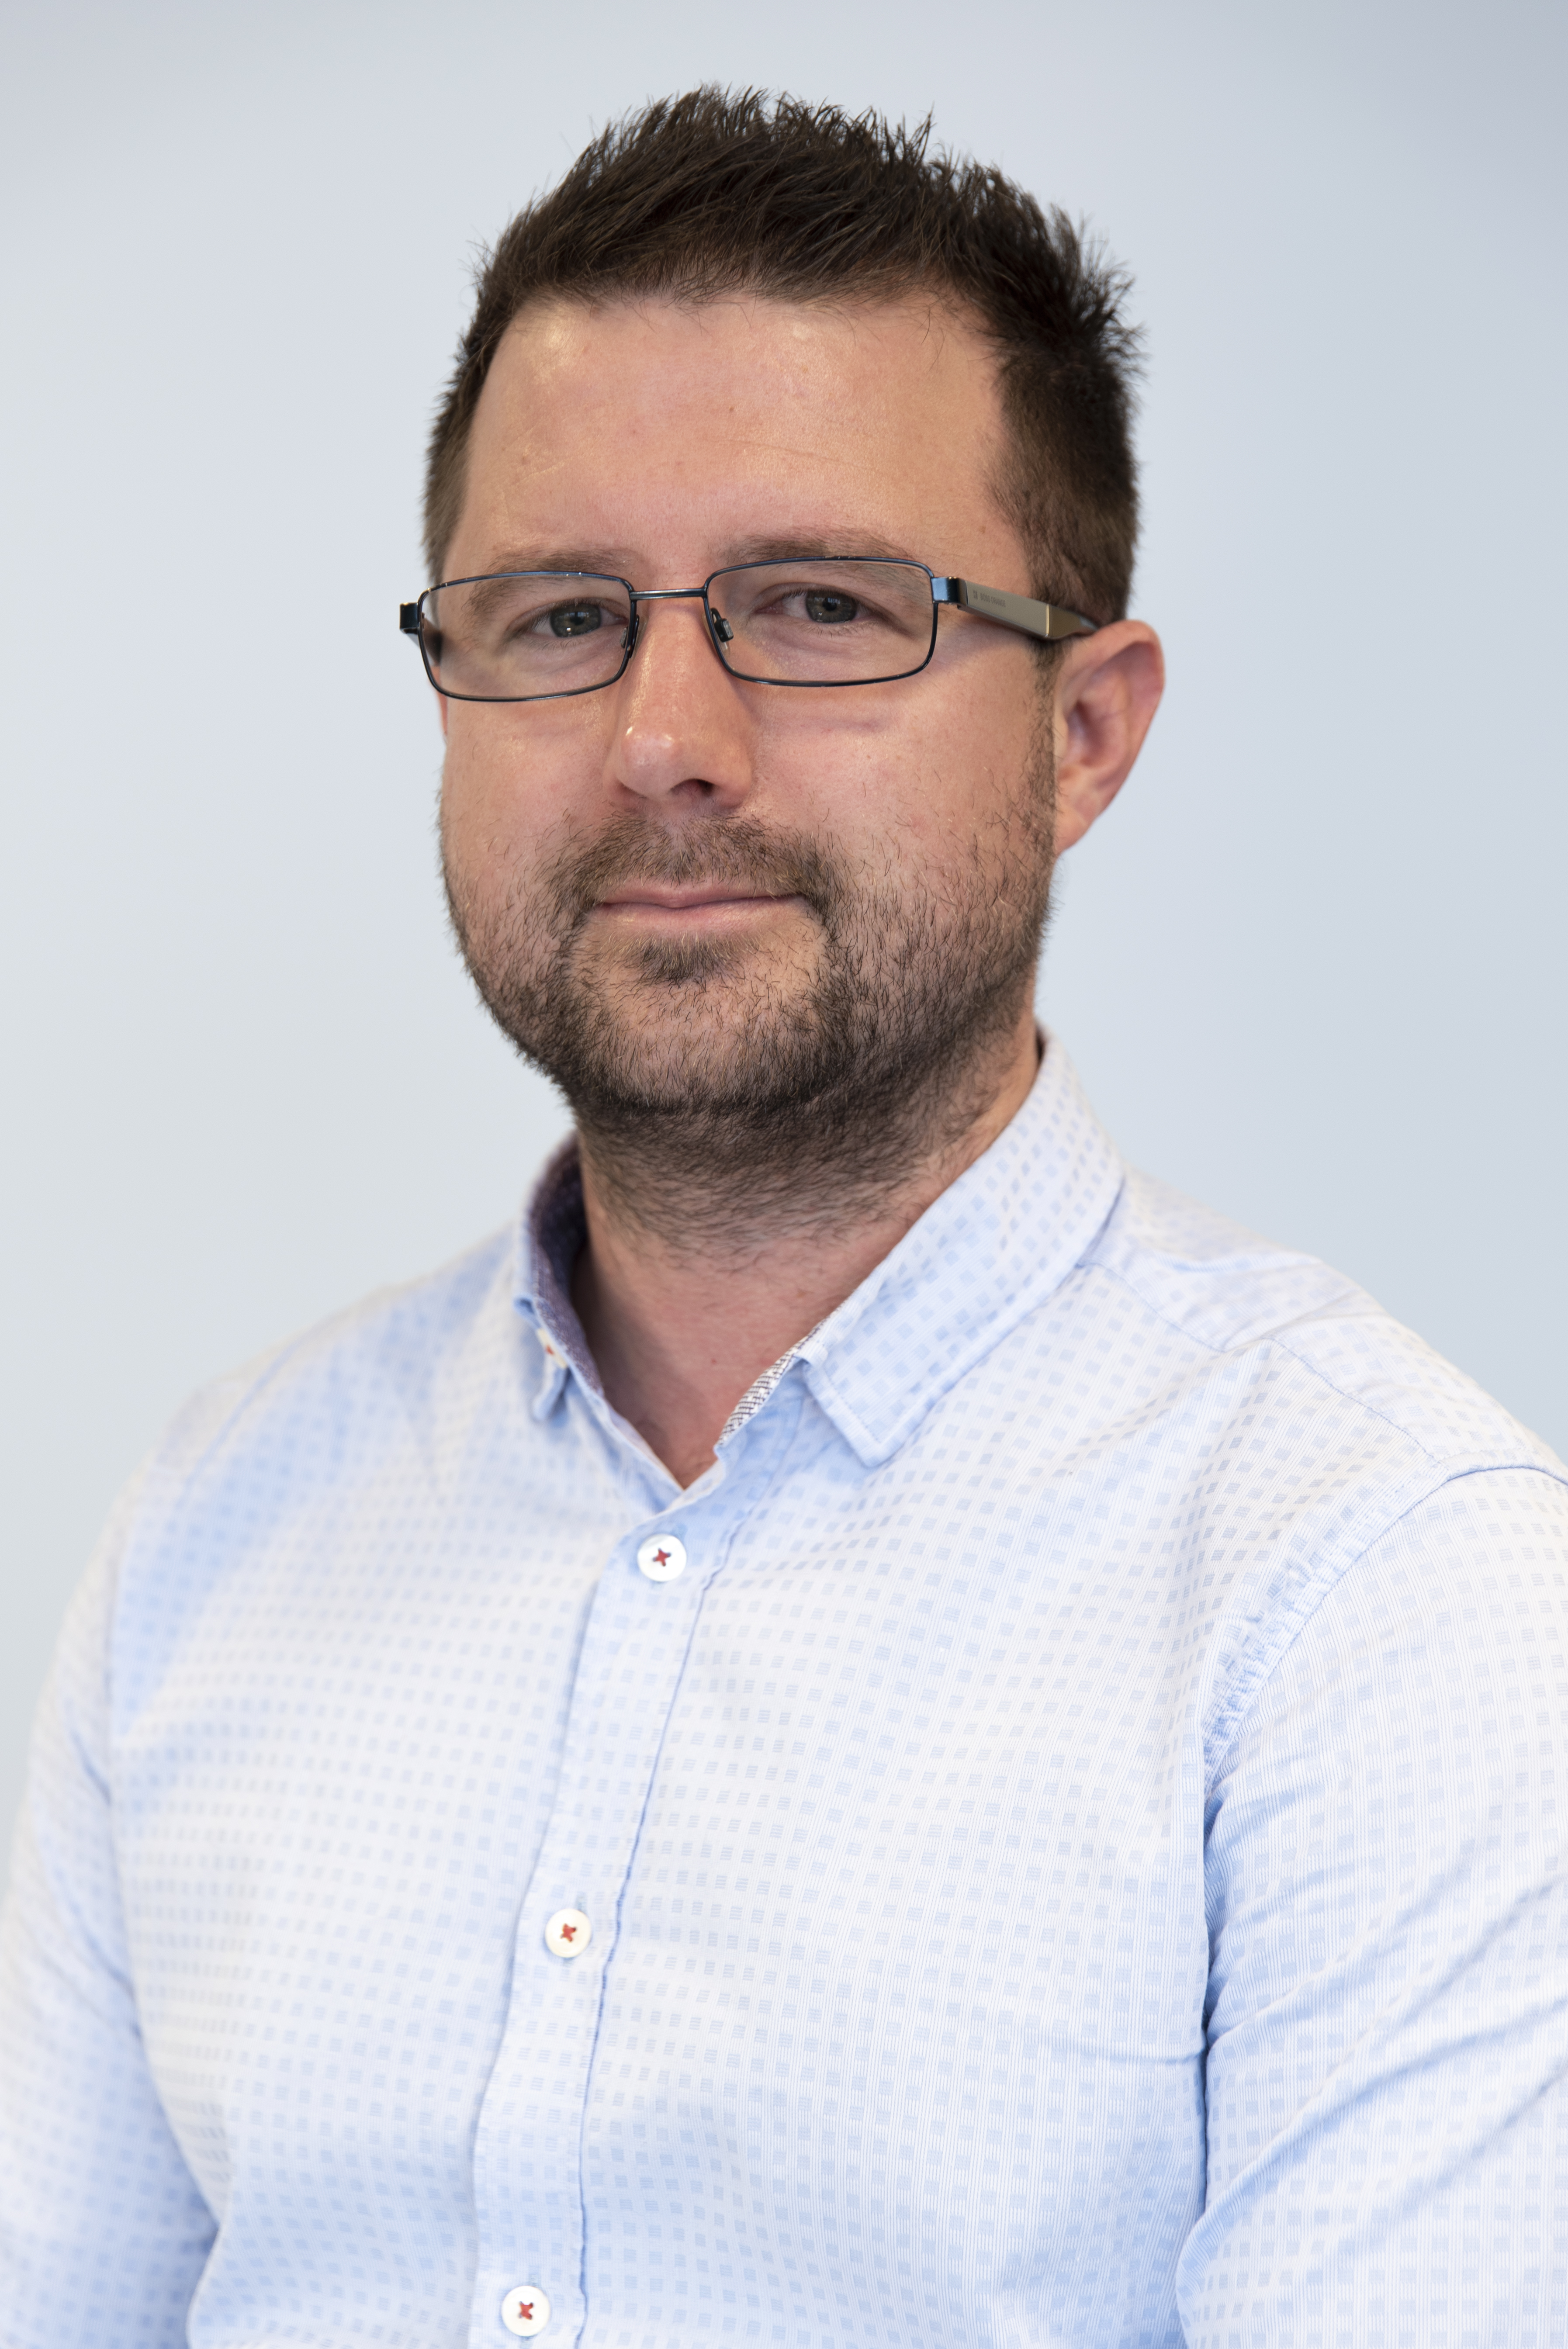
\includegraphics[width=23ex]{AF}
\end{minipage}

\noindent\fcolorbox{red}{lightgray}{%
\begin{minipage}{\dimexpr0.66\textwidth-2\fboxrule-2\fboxsep\relax}   
Dr Umran Ali currently works as a senior lecturer in creative media, and continues to explore virtual natural environment design through teaching and research, maintaining a deep interest in the meaning, impact, and design of natural spaces, in particular around video games. A keen video game collector and player, and a landscape photographer. Holds a PhD in \href{http://usir.salford.ac.uk/id/eprint/39394/?template=banner}{A practice-based exploration of natural environment design in computer \& video games.}
\end{minipage}}%
\begin{minipage}{0.67\textwidth}
\includegraphics[width=23ex]{UA}
\end{minipage}


%----------------------------------------------------------------------------------------
%	BIBLIOGRAPHY
%----------------------------------------------------------------------------------------

\chapterimage{} % Chapter heading image
\chapterspaceabove{2.5cm} % Whitespace from the top of the page to the chapter title on chapter pages
\chapterspacebelow{2cm} % Amount of vertical whitespace from the top margin to the start of the text on chapter pages

%------------------------------------------------

\chapter*{Bibliography}
%\addcontentsline{toc}{chapter}{\textcolor{ocre}{Bibliography}} % Add a Bibliography heading to the table of contents

\printbibliography

%\section*{Articles}
%\addcontentsline{toc}{section}{Articles} % Add the Articles subheading to the table of contents

%\printbibliography[heading=bibempty, type=article] % Output article bibliography entries

%\section*{Books}
%\addcontentsline{toc}{section}{Books} % Add the Books subheading to the table of contents

%\printbibliography[heading=bibempty, type=book] % Output book bibliography entries

%----------------------------------------------------------------------------------------
%	INDEX
%----------------------------------------------------------------------------------------

\cleardoublepage % Make sure the index starts on an odd (right side) page
\phantomsection
\addcontentsline{toc}{chapter}{\textcolor{ocre}{Index}} % Add an Index heading to the table of contents
\printindex % Output the index

\end{document}
